
\documentclass[energies,article,submit,moreauthors,noheaderline]{Definitions/mdpi}


\firstpage{1}
\makeatletter
\setcounter{page}{\@firstpage}
\makeatother
\pubvolume{1}
\issuenum{1}
\articlenumber{0}
\pubyear{2026}
\copyrightyear{2026}
\datereceived{ }
\daterevised{ }
\dateaccepted{ }
\datepublished{ }

% Additional packages and local commands used by the converted manuscript.
\usepackage{adjustbox}
\usepackage{makecell}
\usepackage{longtable}
\usetikzlibrary{arrows.meta,positioning,shapes.geometric}
% Compensate for fancyhdr header height warning.
\setlength{\headheight}{20.0pt}
\addtolength{\topmargin}{-8.0pt}
\makeatletter
\def\LT@output{%
  \ifnum\outputpenalty <-\@Mi
    \ifnum\outputpenalty > -\LT@end@pen
      \LT@err{floats and marginpars not allowed in a longtable}\@ehc
    \else
      \setbox\z@\vbox{\unvbox\@cclv}%
      \ifdim \ht\LT@lastfoot>\ht\LT@foot
        \dimen@\pagegoal
        \advance\dimen@-\ht\LT@lastfoot
        \ifdim\dimen@<\ht\z@
          \setbox\@cclv\vbox{\unvbox\z@\copy\LT@foot\vss}%
          \@makecol
          \@outputpage
          \setbox\@cclv\vbox{\box\LT@head}%
        \fi
      \fi
      \global\@colroom\@colht
      \global\vsize\@colht
      \vbox
        {\unvbox\z@\box\LT@foot}%
    \fi
  \else
    \setbox\@cclv\vbox{\unvbox\@cclv\copy\LT@foot\vss}%
    \@makecol
    \@outputpage
    \global\vsize\@colroom
    \copy\LT@head\nobreak
  \fi}
\makeatother
\newcommand{\degree}{\texorpdfstring{\ensuremath{^\circ}}{\textdegree}}

% Strip math tokens from PDF metadata strings (abstract/title) to avoid
% hyperref "Token not allowed in a PDF string" warnings.
\makeatletter
\AtBeginDocument{%
  \pdfstringdefDisableCommands{%
    \def\ensuremath#1{}%
    \def\textsuperscript#1{#1}%
    \def\textsubscript#1{#1}%
    \def\degree{\textdegree}%
    \def\,{ }%
    \def\thinspace{ }%
    \def\quad{ }%
    \def\geq{>=}%
    \def\leq{<=}%
  }%
}
\makeatother

\Title{Parametric Thermo-Hydraulic Benchmarking of Capsule and Dimple Plate Heat Exchanger Channels via Periodic Unit-Cell CFD}

\Author{Cheuk Sing Cheung \textsuperscript{1}, Christos Skarakis \textsuperscript{1} , Lance Smith \textsuperscript{2}, Jiyuan Tu \textsuperscript{1}, Abhijit Date \textsuperscript{1}, Kiao Inthavong \textsuperscript{1} and Sara Vahaji \textsuperscript{1}}

\AuthorNames{Cheuk Sing Cheung, Christos Skarakis, Sara Vahaji, Lance Smith and Kiao Inthavong}

% Affiliations / Addresses
\address{%
\textsuperscript{1} \quad School of Engineering, RMIT University, Melbourne, VIC 3000, Australia\\
\textsuperscript{2} \quad InKorr Pty Ltd, Knoxfield, VIC 3180, Australia}

% Contact information of the corresponding author
\corres{Correspondence: kiao.inthavong@rmit.edu.au}

% Abstract (single paragraph)
\abstract{Direct comparisons between capsule- and dimple-embossed plate heat exchanger channels are limited by differences in operating conditions and metric definitions across published studies. This study addresses that comparison gap through a side-by-side assessment under a common steady-state, single-phase water-flow Reynolds-averaged Navier--Stokes framework, unit-cell approach, thermal boundary conditions and reporting definitions at Re = 4282. Four seven-case sweeps vary capsule angle, capsule height, dimple height and dimple flow-entry angle; one additional case combines the largest tested dimple height and angle. The unit cells use lateral periodic boundaries and a streamwise quasi-periodic iteration loop for velocity and turbulence profiles, while inlet temperature remains prescribed. The performance evaluation criterion (PEC) combines the two-wall Nusselt number with the Fanning friction factor to quantify the heat-transfer--flow-resistance trade-off. The heat-transfer coefficient uses both walls' total heat rate and area, referenced to each case's fluid-domain mass-average static temperature. Relative embossing depth (RED) is height divided by the case-specific hydraulic diameter. Constructed PEC ranges are 254.6--273.0 for capsule angle, 254.8--294.6 for capsule height, 234.0--285.2 for dimple angle and 214.8--251.0 for dimple height. The combined dimple case gives PEC = 305.14, compared with 294.64 for the 5 mm capsule case. Their 3.56\% separation is not an uncertainty-resolved performance advantage. These are comparative outcomes within the tested parameter ranges and unit-cell heating conditions.}

% Keywords
\keyword{Computational Fluid Dynamics; plate heat exchangers; capsule-type Plate Heat Exchanger; dimple-type Plate Heat Exchanger; heat transfer; performance evaluation criterion}

% Bibliographic source embedded in LaTeX to keep delivery to .tex/.png files.
% BibTeX data below is generated at compilation; no build artifacts are uploaded.
\begin{filecontents*}[overwrite]{energies_revision_sources.bib}
@manual{ansys2025surface,
  author = {{Ansys, Inc.}},
  title = {{Ansys Fluent Theory Guide, Release 2025 R2}},
  organization = {Ansys, Inc.},
  year = {2025},
  note = {Sections 25.1 (Fluxes Through Boundaries), 25.3.1 (Computing Surface Integrals) and 25.4.1 (Computing Volume Integrals), especially Equations 25--16, 25--17 and 25--39; accessed 22 September 2026},
  url = {https://ansyshelp.ansys.com/public/Views/Secured/corp/v252/en/flu_th/flu_th_sec_compute_volint.html}
}
@manual{ansys2025htc,
  author = {{Ansys, Inc.}},
  title = {{Ansys Fluent User's Guide, Release 2025 R2}},
  organization = {Ansys, Inc.},
  year = {2025},
  note = {Sections 17.2.3.5 (Reporting Averaged Heat Transfer Coefficients) and 43.4 (Surface Heat Transfer Coef., Equation 43--50); accessed 20 September 2026},
  url = {https://ansyshelp.ansys.com/public/Views/Secured/corp/v252/en/flu_ug/flu_ug_fvdefs.html}
}
@manual{nistLinearRegression,
  author = {{NIST/SEMATECH}},
  title = {{e-Handbook of Statistical Methods: Linear Least Squares Regression}},
  organization = {National Institute of Standards and Technology},
  note = {Section 4.1.4.1; accessed 20 September 2026},
  url = {https://www.itl.nist.gov/div898/handbook/pmd/section1/pmd141.htm}
}
@article{celik2008gci,
  author = {Celik, Ismail B. and Ghia, Urmila and Roache, Patrick J. and Freitas, Christopher J. and Coleman, Hugh and Raad, Peter E.},
  title = {Procedure for Estimation and Reporting of Uncertainty Due to Discretization in {CFD} Applications},
  journal = {Journal of Fluids Engineering},
  year = {2008},
  volume = {130},
  number = {7},
  pages = {078001},
  doi = {10.1115/1.2960953}
}
@article{du2025,
  author = {Du, Yubin and Wei, Wenjian and Xu, Chengcheng and Wang, Yanfeng and Li, Xiaolu},
  title = {Heat transfer characteristics of single-phase flow through dimple plate heat exchanger},
  journal = {Applied Thermal Engineering},
  volume = {273},
  year = {2025},
  pages = {126499},
  doi = {10.1016/j.applthermaleng.2025.126499}
}
\end{filecontents*}


\begin{document}

% Center body pages for local review without editing the MDPI class file.
\newgeometry{left=2.5cm,right=2.5cm,top=2.0cm,bottom=2.0cm,includehead,includefoot}
\fancyheadoffset[L]{0pt}
\fancyfootoffset[L]{0pt}

\begin{table}[H]
\caption{Nomenclature}
\centering
\scriptsize
\renewcommand{\arraystretch}{1.05}
\begin{tabularx}{\textwidth}{@{}l>{\raggedright\arraybackslash}X@{\quad}l>{\raggedright\arraybackslash}X@{}}
\hline
\textbf{Symbol} & \textbf{Description} & \textbf{Symbol} & \textbf{Description} \\
\hline
$A$         & Cross-sectional flow area (mm$^2$) & Nu          & Nusselt number (--) \\
$A_0$       & Adopted inlet flow area (mm$^2$) & $P$ & Wetted perimeter (mm) \\
$C$         & Unit-cell centre & PEC & Performance evaluation criterion (--) \\
$C_p$       & Specific heat capacity (J/kg$\cdot$K) & Pr          & Prandtl number (--) \\
$D$         & Dimple diameter (mm) & $Q_f$, $Q_j$ & Fluid energy gain; wall-$j$ heat rate (W) \\
$D_e$       & Hydraulic diameter (mm) & Re          & Reynolds number (--) \\
$f$, $f_F$  & Fanning friction factor (--) & $\mathrm{Re}_x$ & Local Reynolds number (--) \\
$h$         & Embossing height (mm) & RED         & Relative Embossing Depth (--) \\
$h_{ave}$ & Two-wall, fluid-temperature-referenced heat-transfer coefficient (W/m$^2\cdot$K) & $S$         & Total heated wall area, $S_1+S_2$ (mm$^2$) \\
$h_c$       & Capsule height (mm) & $T_{f,ave}$ & Fluid-domain mass-average temperature (K) \\
$h_d$       & Dimple height (mm) & $T_{f,in}$ & Fluid inlet temperature (K) \\
$k$         & Turbulence kinetic energy (m$^2$/s$^2$) & $T_{f,out}$ & Fluid outlet temperature (K) \\
$l$         & Capsule length (mm)  & $T_w$       & Wall temperature (K) \\
$l_c$       & Capsule unit-cell length (mm) & $u$         & Prescribed reference mean speed (m/s) \\
$l_d$, $L$  & Dimple/common unit-cell length (mm) & $w$         & Capsule width (mm) \\
$\dot{m}$         & Mass flow rate (kg/s) & $x$         & Streamwise distance (m) \\
$T_{\mathrm{ref}}$ & Coefficient reporting temperature (K) & $y^+$       & Dimensionless wall distance (--) \\
\hline
\multicolumn{2}{l}{\textbf{Greek symbols}} & \multicolumn{2}{l}{\textbf{Abbreviations}} \\
\hline
$\delta$    & Boundary-layer thickness (m) & CFD   & Computational fluid dynamics \\
$\Delta p$  & Pressure drop (Pa) & CPHE  & Capsule-type plate heat exchanger \\
$\Delta\mathrm{PEC}$ & Difference between matched CPHE and DPHE PEC values (--) & & \\
$\epsilon$  & Turbulence dissipation rate (m$^2$/s$^3$) & DPHE  & Dimple-type plate heat exchanger \\
$\theta_c$  & Capsule angle (\degree) & HVAC  & Heating, ventilation, and air-conditioning \\
$\theta_d$  & Dimple angle (\degree) & PHE   & Plate heat exchanger \\
$\lambda$   & Thermal conductivity (W/m$\cdot$K) & RANS  & Reynolds-averaged Navier--Stokes \\
$\rho$      & Fluid density (kg/m$^3$) & SST   & Shear Stress Transport \\
$\upsilon$  & Kinematic viscosity (m$^2$/s) & STHE  & Shell-and-tube heat exchanger \\
$\omega$    & Specific dissipation rate (s$^{-1}$) & TKE   & Turbulence kinetic energy \\          
\hline
\end{tabularx}
\end{table}


\section{Introduction}
\label{sec:introduction} 


Plate heat exchangers (PHEs) place a large heat-transfer area within a compact volume and are widely used in power generation, process industries, heating and cooling systems, and refrigeration. Alternating embossed plates form narrow passages that repeatedly disturb the thermal and hydrodynamic boundary layers. This disturbance can strengthen convection and reduce the area required for a specified thermal duty, but the associated separation, recirculation, and wall shear also increase pressure loss and pumping demand. Heat transfer and hydraulic resistance are therefore coupled design objectives: an embossing should not be judged by Nusselt number alone if its thermal gain is obtained at a disproportionate friction penalty \citep{abukhader2012, thulukkanam2013, zhang2019a}. Although chevron plates remain the conventional reference, capsule, dimple, and pillow surfaces provide alternative ways to control the flow path and surface-area distribution.

The capsule studies summarized in Table~\ref{tab:embossing-summary} demonstrate that performance depends on more than the presence of an embossing. \citet{hamedi2024} reported that a symmetric convex--concave capsule arrangement increased Nusselt number by 28--55\% relative to a simple channel, but also increased the friction factor by 35--44\%. Capsule aspect ratio and size further shift this balance: a larger length-to-width ratio can improve energy efficiency, whereas smaller capsules intensify heat transfer and pressure loss \citep{jiang2019a, jiang2020}. Symmetric arrangements have outperformed zig-zag layouts, and capsule surfaces have also produced higher Nusselt numbers with lower friction factors than chevron surfaces under the conditions examined by \citet{zhang2016}. Geometry optimization produced an 8.3\% increase in heat-transfer coefficient together with a 14.3\% reduction in friction \citep{yu2024}, while adding secondary dimples to capsule surfaces increased heat transfer by 19--46\% \citep{shao2024}. Collectively, these results show that capsule orientation, size, aspect ratio, and arrangement can reorganize the thermal--hydraulic trade-off; they do not identify one configuration that remains superior under a different geometry or operating basis.

The dimple and pillow literature shows the same sensitivity to geometry. Pillow plates have required 30\% less heat-transfer area than chevron plates while producing a lower pressure drop \citep{arsenyeva2019}, and a dimpled pillow channel achieved an 11.2\% thermo-hydraulic improvement with an 8.7\% pressure-loss reduction \citep{piper2019}. For standalone dimple surfaces, \citet{soman2022} reported a 39\% Nusselt-number increase relative to a flat PHE, while hemispherical dimples produced a heat-transfer coefficient approximately 27.2\% higher than rhombus dimples \citep{ying2021}. Numerical predictions have also been compared with experiments for several dimple channels, including deviations of $-11\%$ to 1.8\% in one study series \citep{mocnik2020, mocnik2023, mocnik2024}. Other investigations considered supercritical CO$_2$, nanofluids, lubricating oil, two-phase flow, or hybrid capsule--dimple plates \citep{jing2019, li2019, soman2019, torre2019, shao2024}. These results confirm that dimple shape, channel configuration, and working fluid all influence the balance between heat transfer and pressure loss.

Table~\ref{tab:embossing-summary} thus provides strong evidence for both embossing families, but it also exposes the comparison gap. The reported studies use different fluids, Reynolds-number ranges, channel domains, boundary conditions, hydraulic-diameter definitions, turbulence models, reference surfaces, and performance measures. Some investigate single-phase water, whereas others consider nanofluids, supercritical fluids, or multiphase flow; some report Nusselt number and friction factor separately, whereas others use a combined thermo-hydraulic index. Consequently, the published percentage improvements cannot be ranked on a common scale. Most studies also vary parameters within one surface family, leaving it unclear whether the performance of CPHE and DPHE channels responds similarly when angle and height are changed over comparable ranges.

A controlled computational fluid dynamics (CFD) study is suitable for resolving this gap because it provides both integral performance measures and spatial evidence of the mechanisms that produce them. Nusselt number and pressure loss quantify the overall thermal and hydraulic response, while turbulence kinetic energy, streamlines, and temperature fields reveal how an embossing redirects flow, forms wakes, and transports heat from the wall to the channel core. Periodic unit cells have been used successfully for repeating capsule and dimple geometries because they retain the local embossing-induced mechanisms while avoiding the cost of modelling an entire exchanger \citep{hamedi2024, jiang2019a, jiang2020, piper2019, shao2024}. Published comparisons with experiments also support the use of steady RANS modelling for this class of channel \citep{mocnik2020, mocnik2023, mocnik2024}. The SST $k$--$\omega$ model is selected because its near-wall treatment and response to adverse pressure gradients are suited to the separated flows produced by embossed passages \citep{kanaris2006, menter1994}.

The present study therefore benchmarks capsule-type plate heat exchanger (CPHE) and dimple-type plate heat exchanger (DPHE) channels within one steady-state, single-phase water-flow RANS framework at $\mathrm{Re}=4282$. Both geometries use a periodic unit cell, common thermal and hydraulic boundary conditions, and the same hydraulic-diameter definition, so the effects of geometry are not obscured by a change in the numerical basis. Twenty-eight one-factor cases comprise four seven-case sweeps. Capsule and dimple angles cover $0\degree$--$45\degree$ in $7.5\degree$ increments, while capsule and dimple heights cover 2.0--5.0~mm in 0.5~mm increments; the remaining geometric variables are held at the reference values listed in Table~\ref{tab:geom_cases}. This design separates the effects of capsule angle ($\theta_c$), capsule height ($h_c$), dimple height ($h_d$), and dimple flow-entry angle ($\theta_d$). One additional case combines $\theta_d=45\degree$ with $h_d=5.0$~mm to test a targeted dimple interaction identified from the one-factor results, rather than treating the four sweeps as a full factorial optimization.

The study has three objectives: to quantify how the four geometric variables change Nusselt number and the friction factor; to explain those changes using the computed flow and temperature fields; and to compare CPHE and DPHE cases through the performance evaluation criterion (PEC) and relative embossing depth (RED). PEC expresses the heat-transfer--friction trade-off on a common scale, while RED relates embossing height to the effective channel size. This common framework permits a direct benchmark that the heterogeneous literature cannot provide. The finite sweeps and single combined case nevertheless support conclusions only for the tested geometry, fluid, Reynolds number, and boundary conditions; they do not establish a global optimum across untested parameter interactions.

{\footnotesize
\setlength{\LTleft}{0pt}
\setlength{\LTright}{0pt}
\setlength{\LTpre}{0pt}
\setlength{\LTpost}{0pt}
\begin{longtable}{@{}>{\raggedright}p{2.6cm} >{\raggedright}p{1.6cm} >{\raggedright}p{1.6cm} >{\raggedright\arraybackslash}p{8.9cm}@{}}
\caption{Summary of embossing surface enhancement of PHEs}
\label{tab:embossing-summary} \\
\hline
\textbf{Author} & \textbf{Surface} & \textbf{Method\textsuperscript{a}} & \textbf{Key Findings} \\
\hline
\endfirsthead
\caption[]{(continued)} \\
\hline
\textbf{Author} & \textbf{Surface} & \textbf{Method\textsuperscript{a}} & \textbf{Key Findings} \\
\hline
\endhead
\hline
\endfoot
\citet{hamedi2024} & Capsule & E \& N & Proposed a symmetrical arrangement of convex and concave capsule surfaces. Relative to a simple channel, the friction factor increased by 35--44\% and the Nusselt number by 28--55\%. \\
\citet{jiang2019a} & Capsule & N & Found that the capsule length-to-width ratio controls the performance trade-off: a larger ratio improves energy efficiency, while a smaller ratio increases heat transfer and pressure drop. \\
\citet{jiang2020} & Capsule & N & A symmetrical capsule arrangement outperformed a zig-zag arrangement. Smaller capsules increased heat transfer, while larger capsules reduced pressure loss. \\
\citet{jiang2019} & Capsule & E & Found that plate-corrugation geometry had little effect on liquid and gas distribution during two-phase channel flow. \\
\citet{zhang2016} & Capsule & E \& N & Capsule embossing produced a higher Nusselt number and lower friction factor than chevron surfaces. \\
\citet{yu2024} & Capsule & N & Combined CFD with backpropagation optimization, increasing the heat-transfer coefficient by 8.3\% and reducing friction by 14.3\%. \\
\citet{shao2024} & Capsule / Dimple & N & Adding secondary dimples to capsule surfaces increased heat transfer by 19--46\%. \\
\citet{arsenyeva2019} & Pillow & E \& N & Required 30\% less heat-transfer area than chevron plates and produced a lower pressure drop. \\
\citet{shirzad2019a} & Pillow & N & Greater channel height was most efficient at low Reynolds numbers, while wider transverse welding-spot spacing was most efficient at high Reynolds numbers. \\
\citet{shirzad2019b} & Pillow & N & Predicted higher thermal performance with a nanofluid than with water. \\
\citet{kumar2019} & Pillow & N & Numerically examined heat transfer and fluid flow in a pillow-plate channel. \\
\citet{piper2019} & Pillow / Dimple & N & Reported an 11.2\% improvement in thermo-hydraulic performance and an 8.7\% reduction in pressure loss. \\
\citet{jing2019} & Dimple & N & Numerically examined supercritical CO$_2$ flow and heat transfer in rectangular channels with teardrop dimples. \\
\citet{li2019} & Dimple & E & Found that smaller air bubbles produced greater heat transfer than medium or large bubbles during two-phase flow. \\
\citet{mocnik2020} & Dimple & E \& N & Compared turbulence models with experimental data and identified two flow regimes. \\
\citet{mocnik2023} & Dimple & E \& N & Reported numerical results from $-$11\% to 1.8\% relative to the experiments. \\
\citet{mocnik2024} & Dimple & E \& N & Found good agreement between numerical and experimental results for low-Reynolds-number flow in a dimple-type PHE. \\
\citet{soman2019} & Dimple & E & Nanofluids improved heat transfer relative to water without increasing the friction factor. \\
\citet{soman2022} & Dimple & N & A dimple PHE increased the Nusselt number by 39\% relative to a flat PHE. \\
\citet{torre2019} & Dimple & E \& N & Obtained satisfactory agreement between experiments and simulations for pressure drop and heat transfer with lubricating oil. \\
\citet{wang2019} & Dimple & N & A dimpled surface reduced pressure drop by 20.57\% and increased net power generation by 173.6\%. \\
\citet{ying2021} & Dimple & E \& N & Hemispherical dimple channels produced a heat-transfer coefficient about 27.2\% higher than rhombus dimple channels. \\
\hline
\multicolumn{4}{l}{\textsuperscript{a}E -- Experimental; N -- Numerical}
\end{longtable}
}

\section{Methodology}
\label{sec:methodology}

This numerical investigation applies a common computational fluid dynamics (CFD) framework to benchmark the thermo-hydraulic performance of CPHE and DPHE channels. The method combines periodic unit-cell representation, mesh-independence testing, literature-supported turbulence modelling, and controlled parametric sweeps \citep{jiang2019, mocnik2020}. The calculation sequence is case selection and geometric-domain construction, mesh generation with near-wall prism layers, physical-model and boundary-condition assignment, steady solution through the streamwise quasi-periodic iteration loop, and consistent reduction of the saved fields to thermal and hydraulic metrics. Section~\ref{sec:periodic_boundary} and Scheme~\ref{scheme:simulation-workflow} distinguish the solver iterations within each period from the outlet-to-inlet profile-transfer loop between periods.

\subsection{Numerical methods}
\label{sec:numerical_methods}

The Reynolds-averaged Navier--Stokes (RANS) approach is widely used in numerical studies of capsule and dimple channels. Published models include realizable $k$--$\epsilon$ \citep{kumar2019, jing2019, mocnik2020, mocnik2024}, shear stress transport (SST) $k$--$\omega$ \citep{hamedi2024, jiang2019a, jiang2020, mocnik2020, mocnik2024, torre2019}, Reynolds stress \citep{shao2024, mocnik2023}, elliptic-blending $k$--$\epsilon$ \citep{arsenyeva2019, piper2019}, and standard $k$--$\epsilon$ \citep{soman2022}. The SST $k$--$\omega$ model is used here because it combines near-wall $k$--$\omega$ treatment with a $k$--$\epsilon$ formulation away from the wall and is suited to separated flows with adverse pressure gradients \citep{kanaris2006, khail2023, menter1994}.

All simulations use steady-state, single-phase water flow at subcritical pressure and temperature.

The channel scale is defined using the adopted unit-cell hydraulic-diameter convention,
\begin{equation}
D_e=\frac{4A_0 L}{S},\qquad S=S_1+S_2 ,
\label{eq:De}
\end{equation}
where $A_0$ is the inlet flow area used in the saved cases, $L=l_c=l_d=25$~mm is the inlet-to-outlet cell length, and $S_1$ and $S_2$ are the two wetted, heated wall areas. This is an effective passage-scale definition: replacing the wetted perimeter in the usual $4A/P$ expression by $S/L$ gives Equation~\eqref{eq:De} \citep{zohuri2017,thulukkanam2013}. It should not be interpreted as a local hydraulic diameter at every cross-section of the embossed passage. Its numerical value is evaluated separately from each saved mesh.

The Reynolds number follows the standard definition \citep{cengel2014,thulukkanam2013},
\begin{equation}
\mathrm{Re}=\frac{uD_e}{\upsilon},\qquad \upsilon=\frac{\mu}{\rho}.
\label{eq:Re}
\end{equation}
The prescribed reference speed is therefore $u=4282\mu/(\rho D_e)$. Equal Reynolds number does not imply equal speed when $D_e$ varies: the saved cases give $u=0.308$--$0.679$~m/s. This is the reference mean speed used to scale the recycled velocity-component profiles, not an assumption of a uniform inlet profile or a substitution for the inlet-normal bulk velocity.

Fanning friction factor is adopted in this study, denoted $f_F$ (or simplified as $f$ in the plots). \citep{cengel2014,thulukkanam2013}
\begin{equation}
f_F=\frac{\Delta p\,D_e}{2\rho L u^2}.
\label{eq:f}
\end{equation}
Here $\Delta p$ is the difference between the area-averaged static pressures at the inlet and outlet. Thus the factor 2 in the denominator is intentional for the Fanning convention. All walls are stationary, no-slip and hydraulically smooth.

For constant $C_p$ and balanced inlet and outlet mass flow, the net fluid energy gain follows the steady-flow calorimetric balance \citep{thulukkanam2013,jiang2019a},
\begin{equation}
Q_f=\dot m C_p\left(T_{f,out}^{(E)}-T_{f,in}^{(E)}\right).
\label{eq:Q}
\end{equation}
Here $b\in\{in,out\}$ identifies the inlet or outlet boundary. For constant $C_p$, the energy-balance temperature is the signed temperature flow rate divided by the net mass flow \citep[Section~25.3.1, Equations~25--16 and~25--17]{ansys2025surface}:
\[
T_{f,b}^{(E)}=\frac{\sum_{i\in b}\dot m_i T_i}{\sum_{i\in b}\dot m_i},
\]
where $\dot m_i$ is the signed face mass flow rate relative to the boundary's outward normal; the net boundary mass flow is nonzero. Where local backflow occurs, conservation is checked using signed enthalpy-flux integrals rather than substituting absolute-flux temperature averages into the calorimetric balance \citep[Section~25.1]{ansys2025surface}. The wall heat rate used below is obtained directly from both heated walls, independently of this diagnostic.

For the reconstructed Nu results in Figure~\ref{figure4} and PEC comparisons in Figures~\ref{figure13}--\ref{figure15}, the case-specific reporting reference is the mass-weighted volume average of static temperature over the entire fluid domain $\Omega_f$, as defined in \citet[Section~25.4.1, Equation~25--39]{ansys2025surface}:
\[
T_{\mathrm{ref}}=T_{f,ave}
=\frac{\int_{\Omega_f}\rho T\,\mathrm{d}V}{\int_{\Omega_f}\rho\,\mathrm{d}V}
=\frac{\sum_{i\in\Omega_f}\rho_i V_i T_i}{\sum_{i\in\Omega_f}\rho_i V_i}.
\]
Here $V_i$, $\rho_i$ and $T_i$ are the volume, density and static temperature of fluid cell $i$. The integral is normalized by the total fluid mass, so $T_{f,ave}$ has units of temperature. It weights the mass contained in each cell, not the mass flow crossing a boundary. For the constant-density water used here, it is identical to the volume-weighted average $\sum_i V_i T_i/\sum_i V_i$. This fluid-domain average is distinct from the signed inlet and outlet temperatures $T_{f,b}^{(E)}$ used in the energy balance; it is not their arithmetic mean or difference.

The average heat-transfer coefficient is obtained by area-weighted averaging of Fluent's built-in \emph{Surface Heat Transfer Coef.} over the union of \texttt{wall\_1} and \texttt{wall\_2}, with the Reference Values temperature set to the case-specific $T_{f,ave}$. The equivalent value is reconstructed directly from the saved wall heat fluxes without modifying the original solution files. For the uniform wall temperature $T_w=333$~K, the Fluent field definition and surface-averaging procedure \citep{ansys2025htc} give
\begin{equation}
h_{ave}
=\frac{1}{S_1+S_2}\int_{S_1\cup S_2}
\frac{q''}{T_w-T_{\mathrm{ref}}}\,\mathrm{d}S
=\frac{Q_1+Q_2}{(S_1+S_2)(T_w-T_{f,ave})},
\qquad Q_j=\int_{S_j}q''\,\mathrm{d}S .
\label{eq:h_ave}
\end{equation}
Heat flux is positive from the heated walls into the water. Both wall heat rates and both wall areas therefore enter Equation~\eqref{eq:h_ave}; the individual wall coefficients are not added. This fluid-temperature-based form is consistent with the form of the mean coefficient in \citet{jiang2019a}, while the specific choice of a fluid-domain mass-average reference is defined explicitly here and is not attributed to that paper.

For $\theta_c=0\degree$, the fluid-domain mass-average static temperature is $T_{\mathrm{ref}}=T_{f,ave}=296.1537$~K, giving $h_{ave}=5346.87$~W\,m$^{-2}$\,K$^{-1}$. Across all 29 cases, $T_{f,ave}$ ranges from 295.4045 to 296.7044~K; each case uses its own value. The physical inlet temperature is 293~K and both walls are prescribed at 333~K. The reporting reference does not impose an additional thermal boundary condition or change the solved temperature field, wall heat rates or flow field.

The Nusselt and molecular Prandtl numbers use the standard nondimensional definitions \citep{thulukkanam2013},
\begin{equation}
\mathrm{Nu}=\frac{h_{ave}D_e}{\lambda},
\label{eq:Nu}
\end{equation}
\begin{equation}
\mathrm{Pr}=\frac{\mu C_p}{\lambda}=\frac{\upsilon\rho C_p}{\lambda},
\label{eq:Pr}
\end{equation}
where $\lambda$ is the fluid thermal conductivity. Every case uses the same two-wall averaging and fluid-temperature-reference convention, although the numerical value of $T_{\mathrm{ref}}$ varies with the saved fluid temperatures. This postprocessing definition does not imply thermally periodic temperature profiles.


\subsection{Geometry}
\label{sec:geometry}

Two embossed channel families are considered: capsule and dimple. Both use alternating convex and concave features to disturb the flow, but their planform geometry differs.

The periodic surface is represented by its smallest repeating unit cell. This commonly used approach reduces the computational domain while retaining the flow, thermal, and turbulence mechanisms generated by the repeating embossments \citep{hamedi2024,jiang2019,jiang2020, kumar2019, piper2019, shao2024, zhang2016}.

The local cross-sectional wall profile is generated using the cosine function
\begin{equation}
  y(x)=\frac{h}{2}\left[1+\cos\left(\frac{2\pi x}{D}\right)\right],
  \qquad -\frac{D}{2}<x<\frac{D}{2}.
  \label{eq:cosine_wall_profile}
\end{equation}
Here, $h$ is the profile height and $D$ is the full span of the local profile (the diameter for a dimple). The coordinate $x$ is measured from the profile centre, and $y(x)$ is the displacement from the local reference plane. The profile reaches $y(0)=h$ at its centre and approaches zero at either edge. These are local profile coordinates, distinct from the global CFD coordinate directions.

\begin{figure}[!ht]
\centering
\begin{tabular}{cccc}
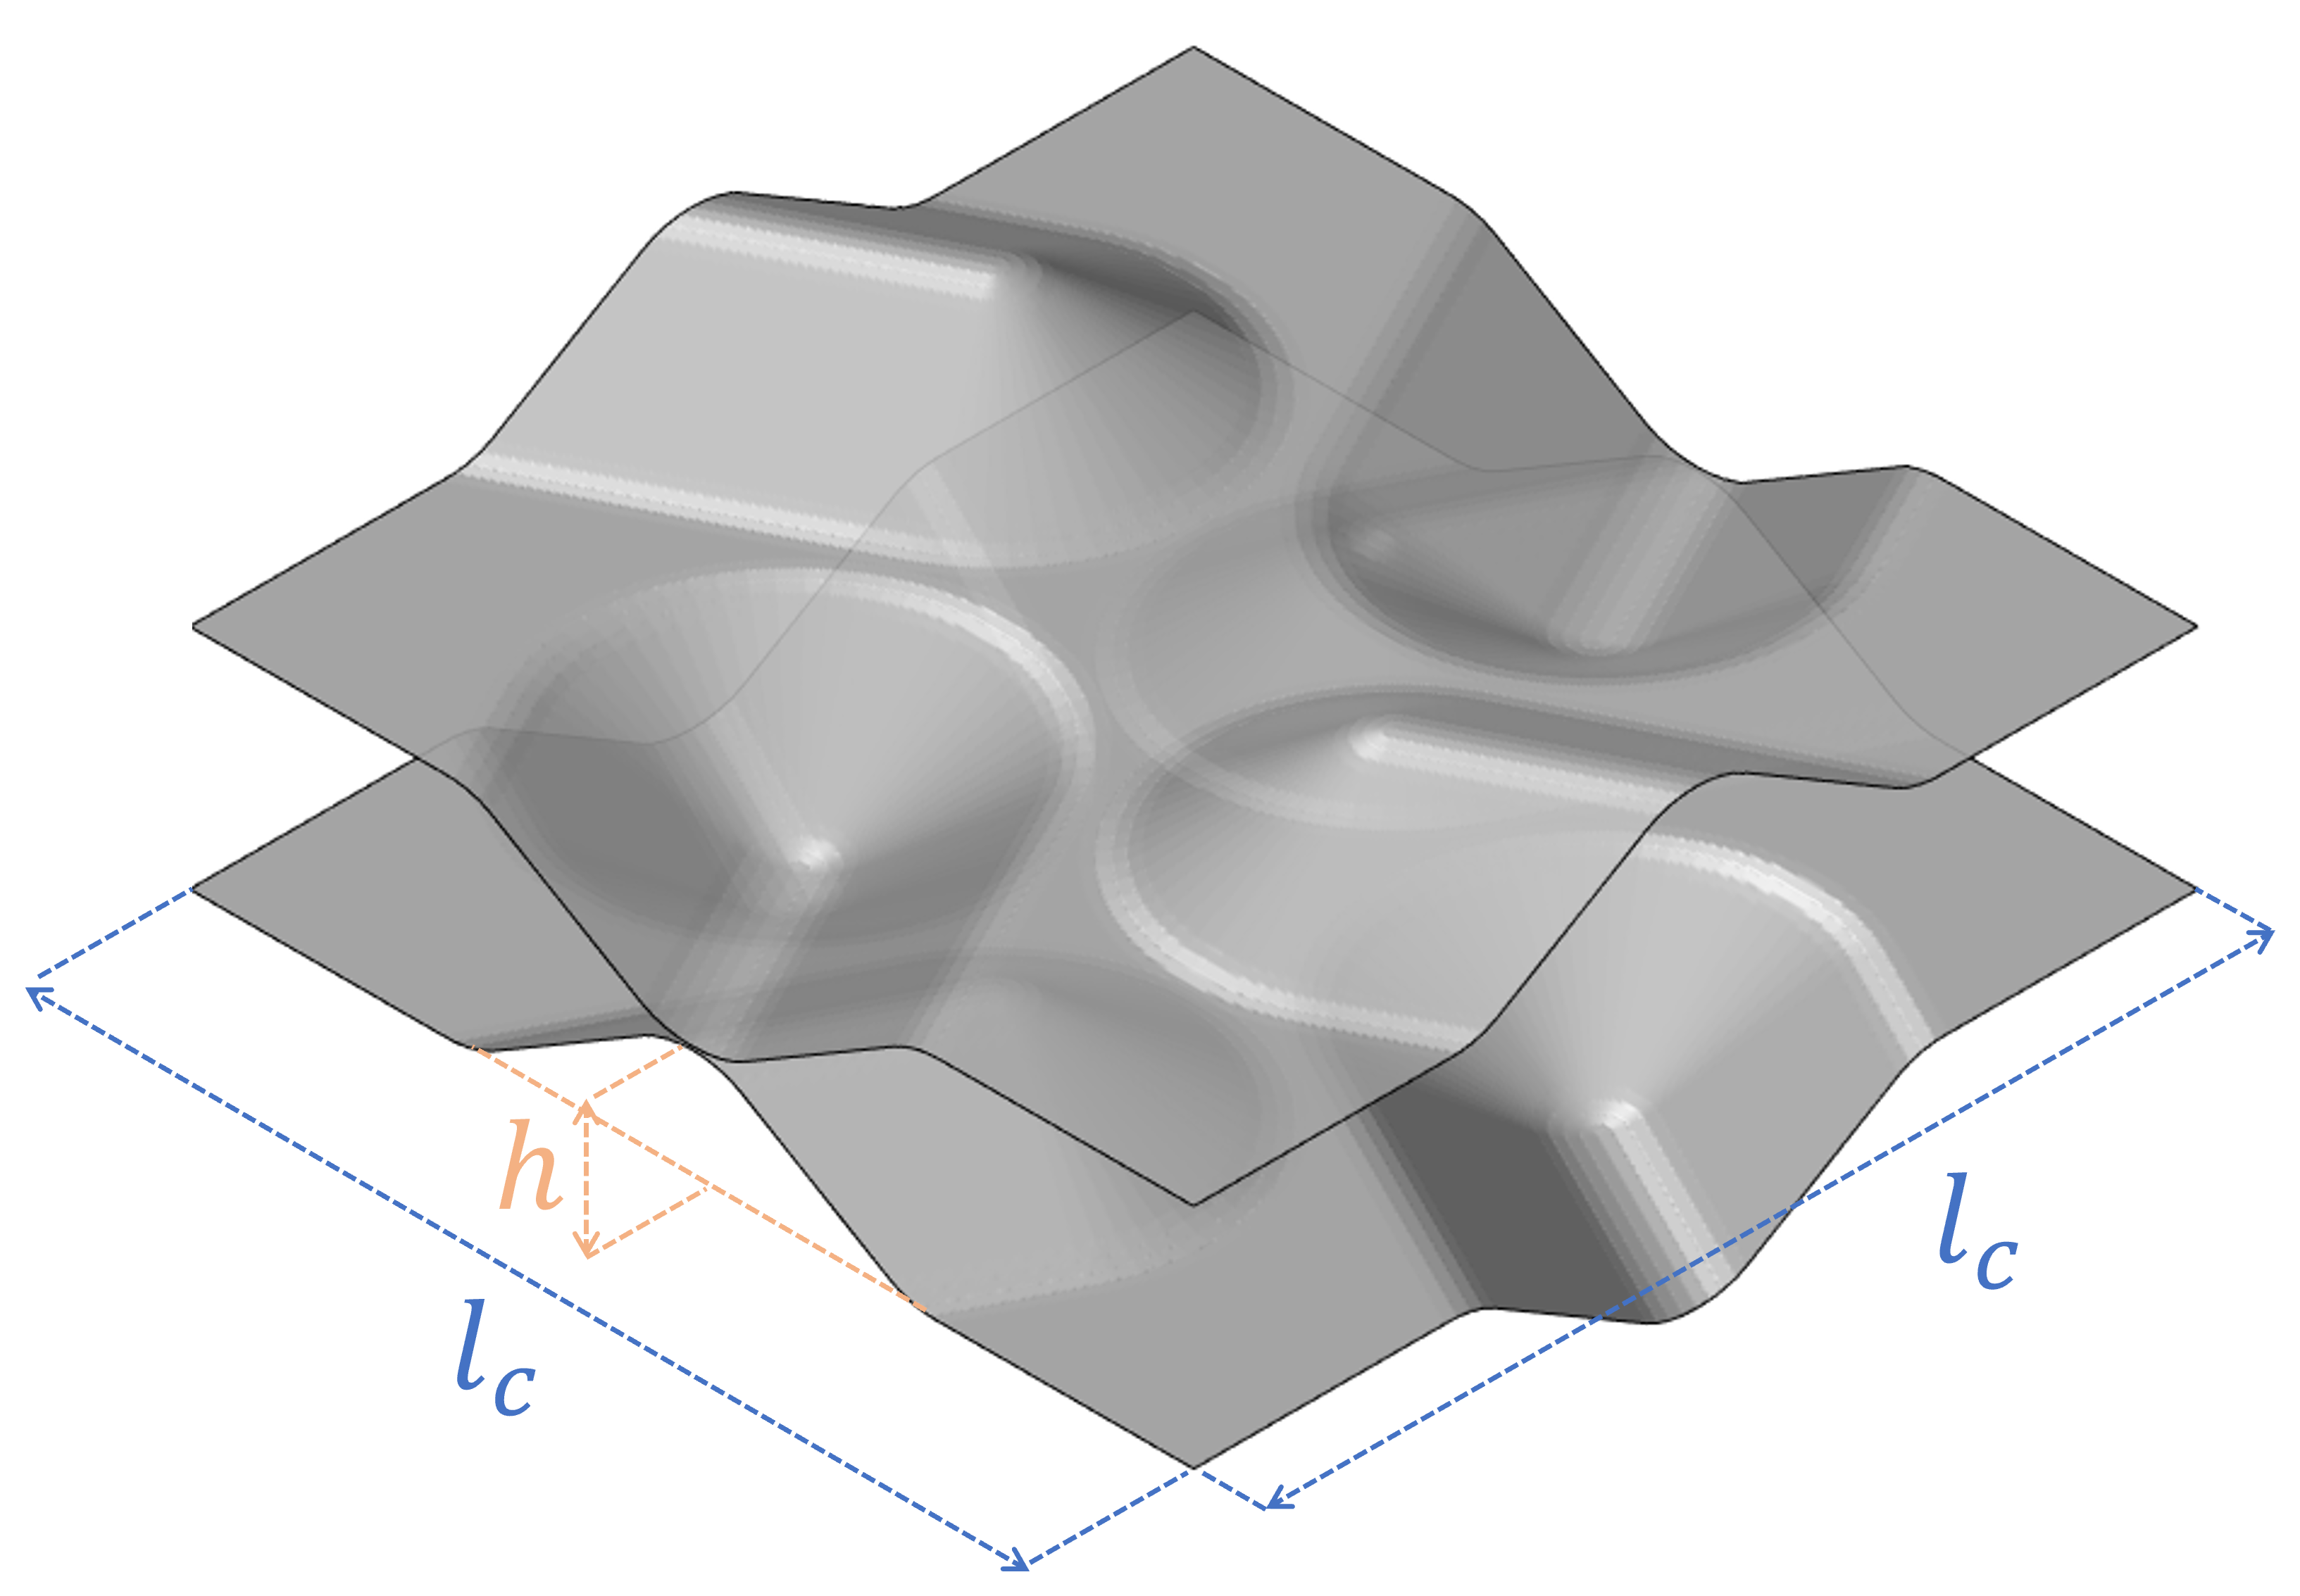
\includegraphics[width=0.3\textwidth]{media/image6_v2.png} &
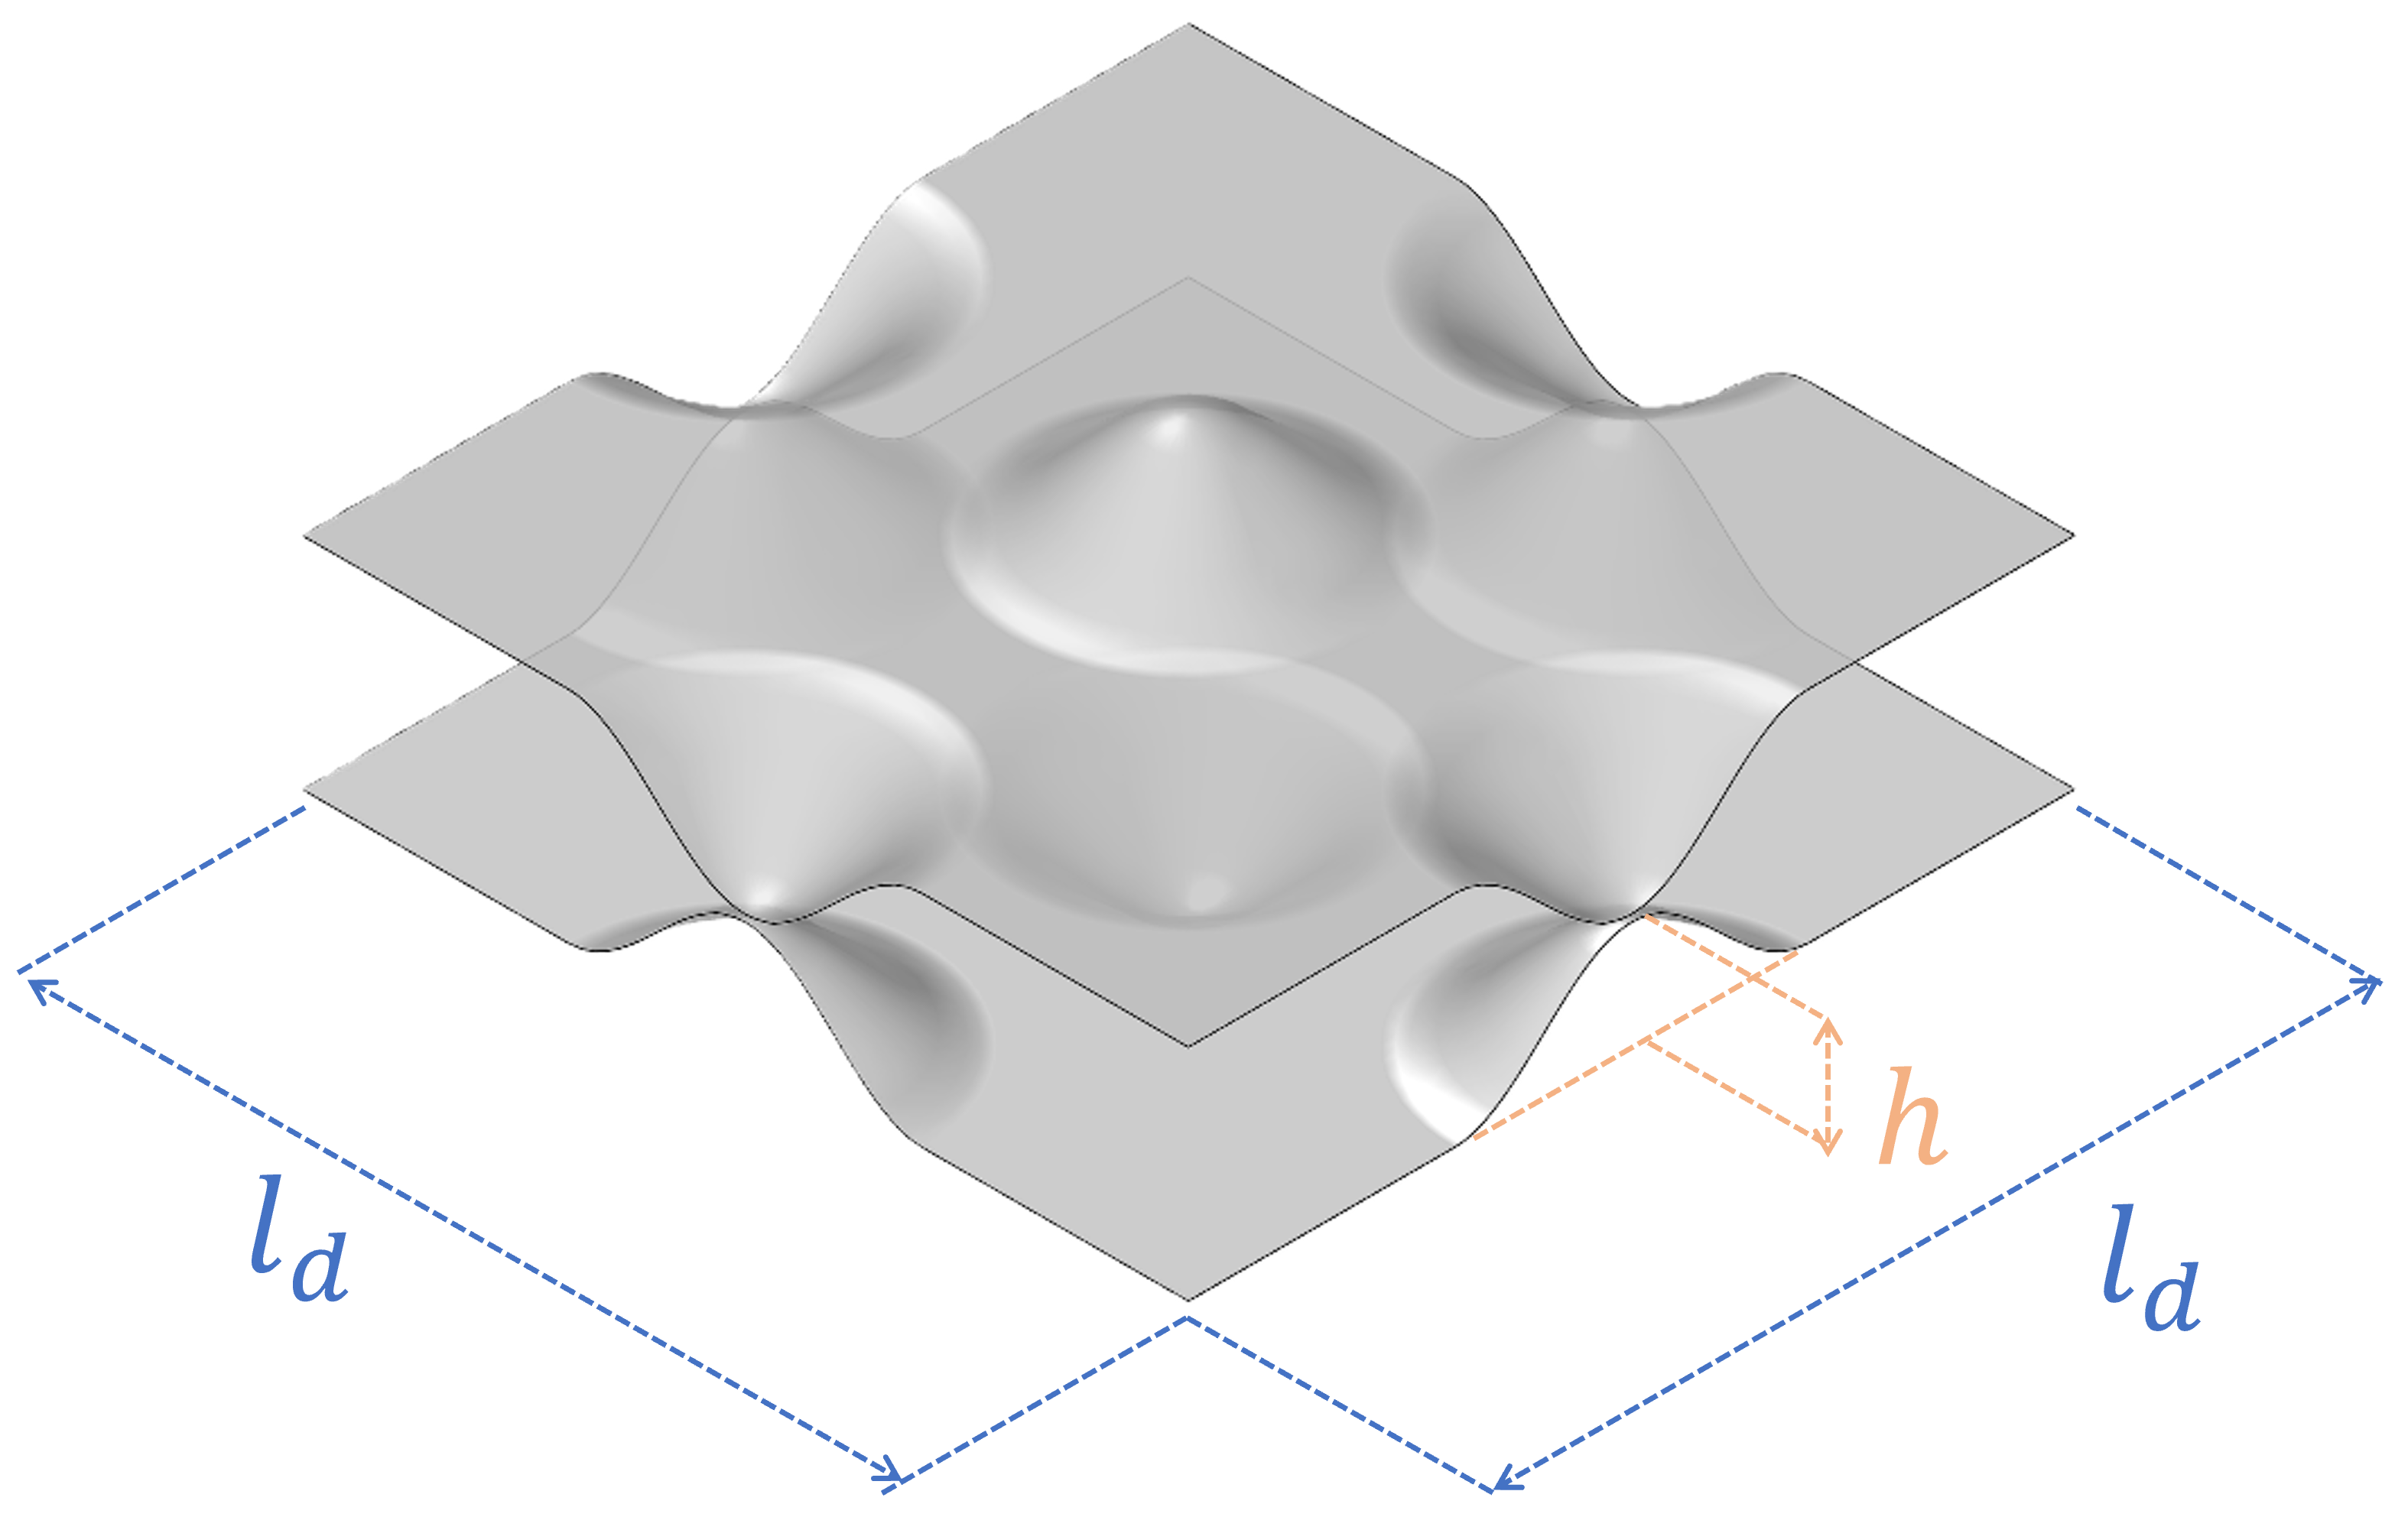
\includegraphics[width=0.3\textwidth]{media/image9_v2.png} &
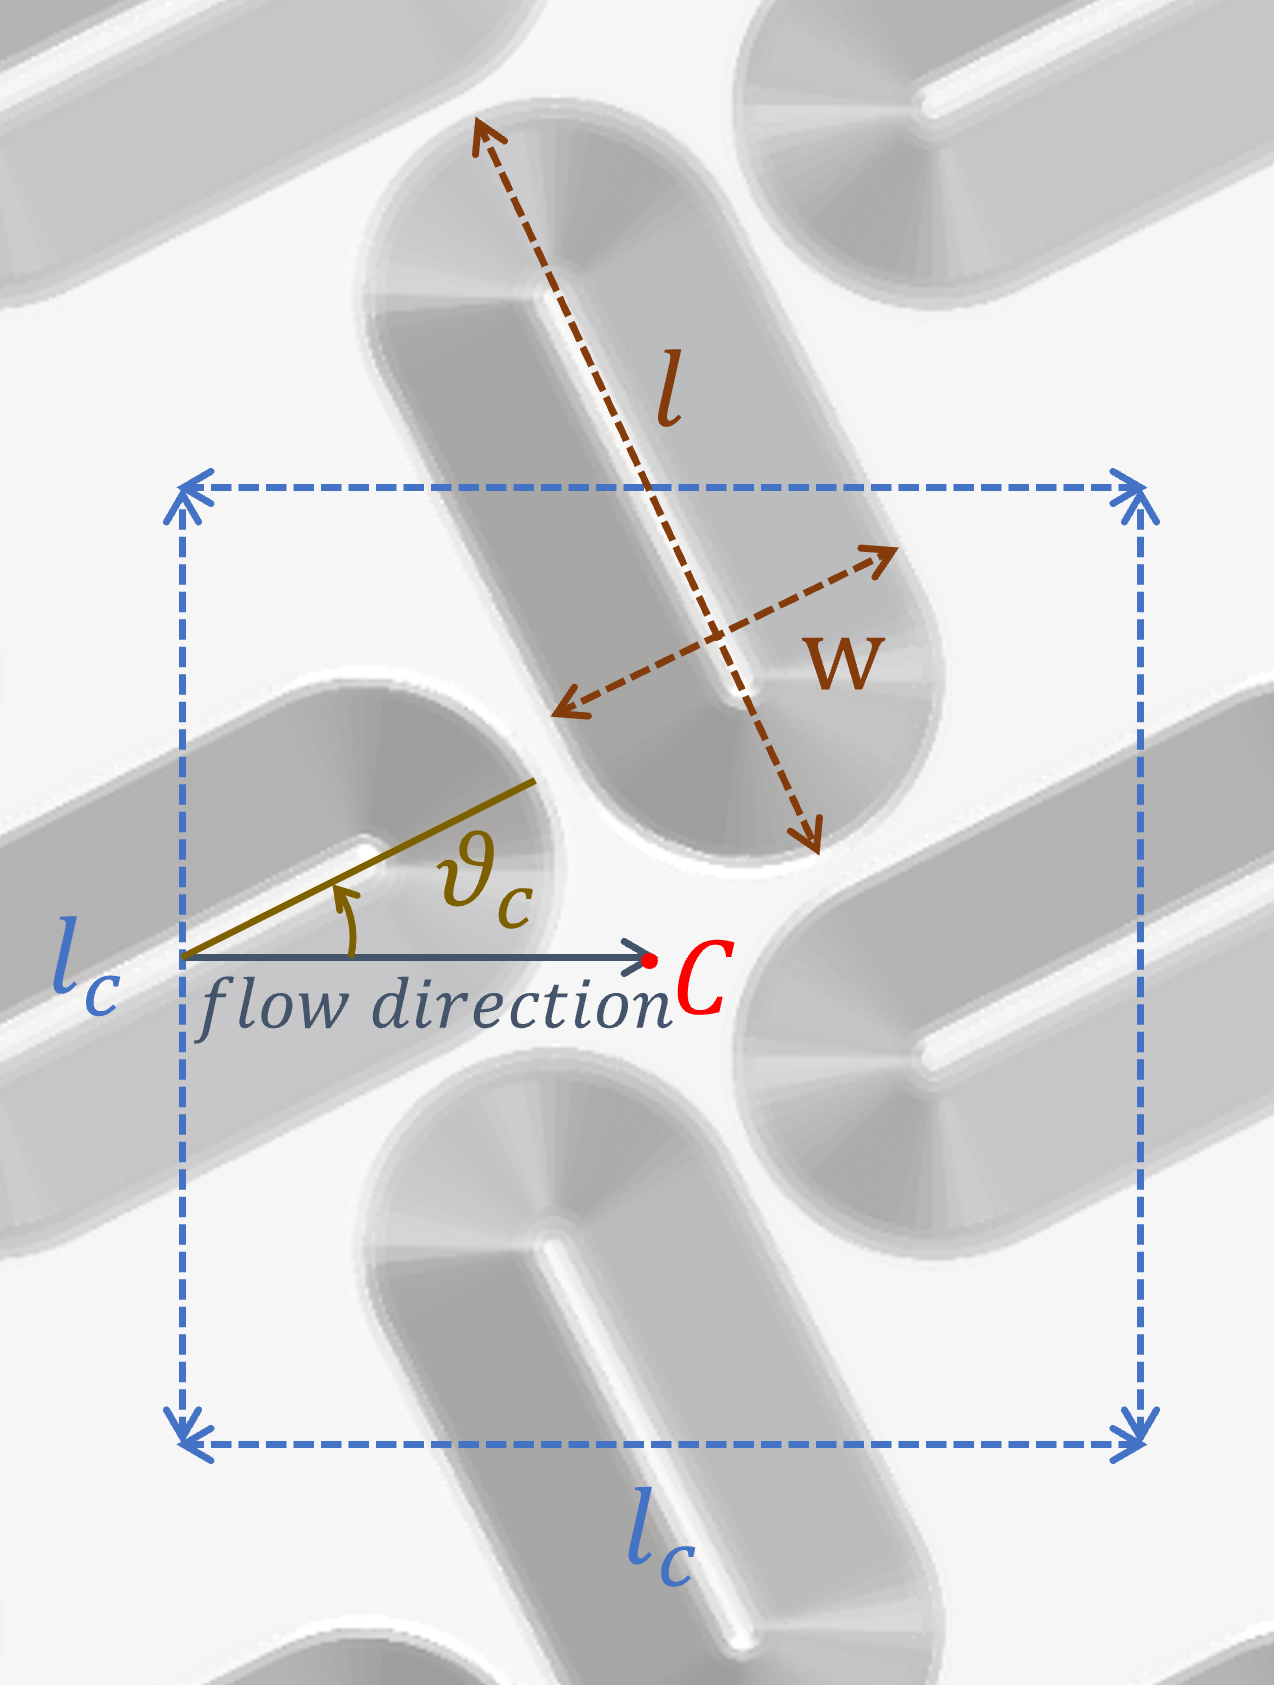
\includegraphics[width=0.2\textwidth]{media/image7_v2.png} &
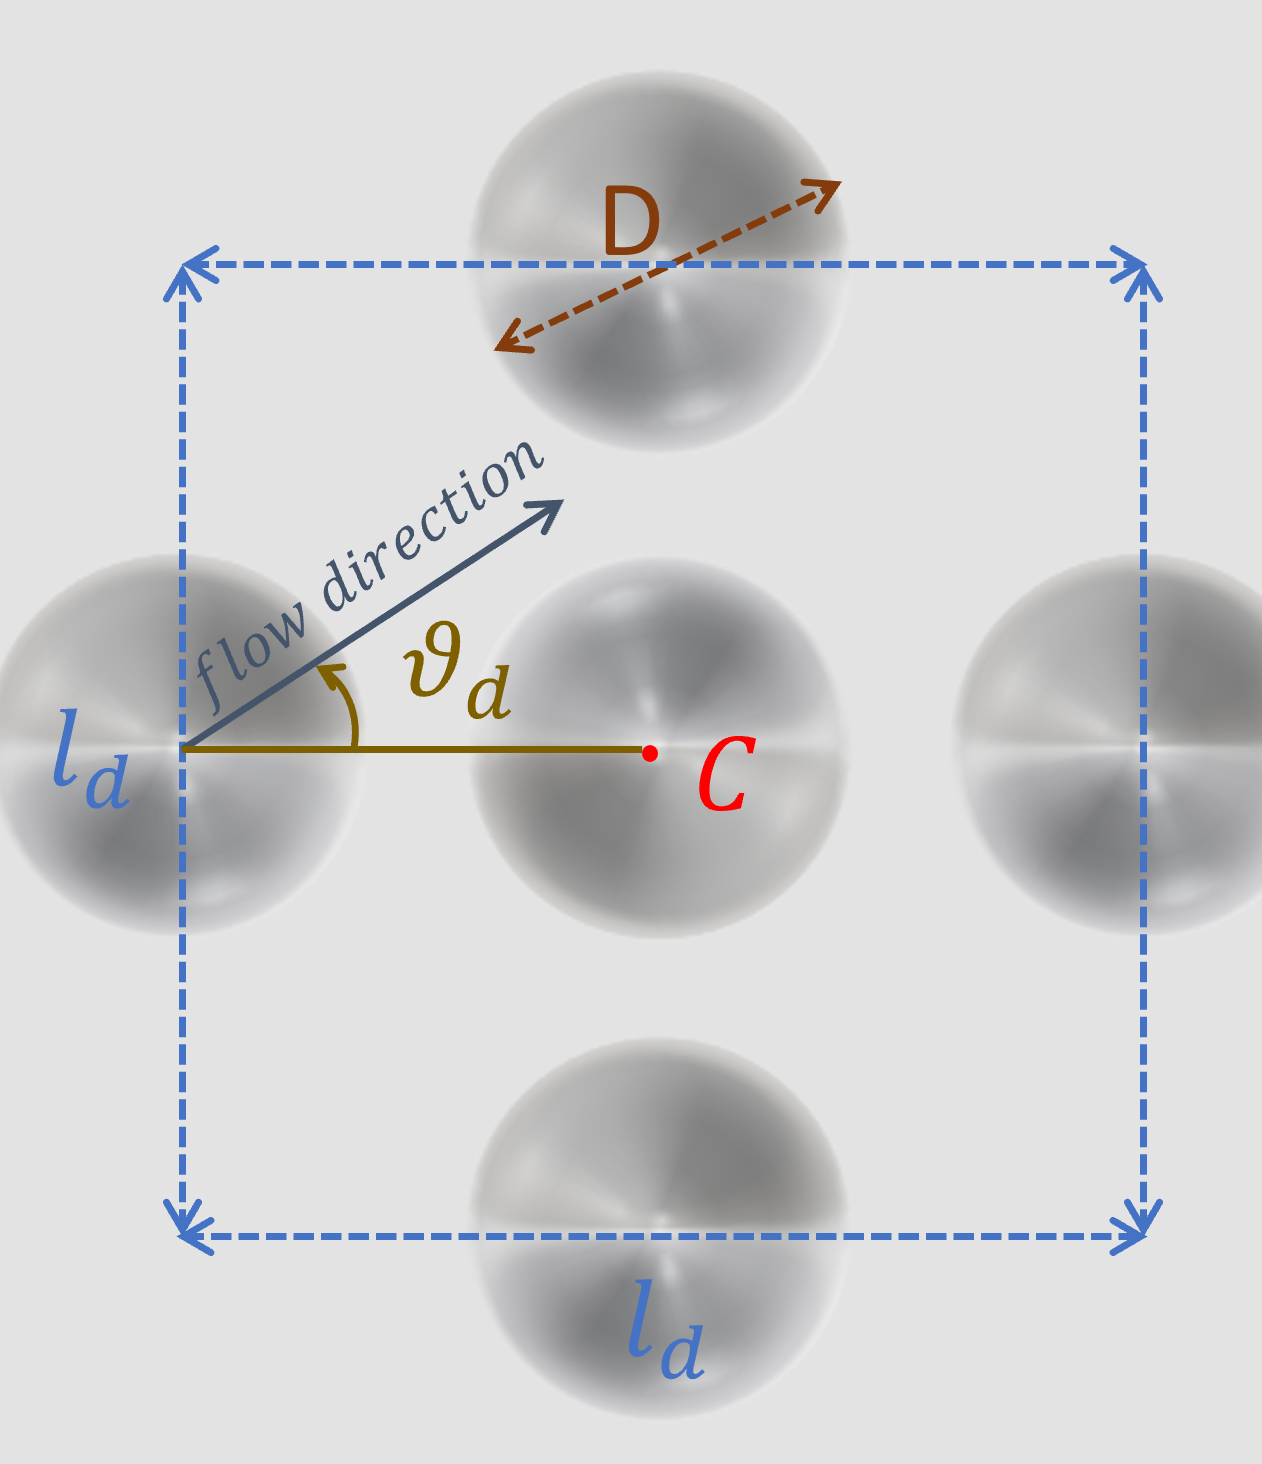
\includegraphics[width=0.2\textwidth]{media/image7.5_v2.png} \\
\end{tabular}
\caption{Unit Cell Dimensions}
\label{figure1}
\end{figure}

\begin{figure}[!ht]
  \centering
  \begin{tabular}{@{}cc@{}}
    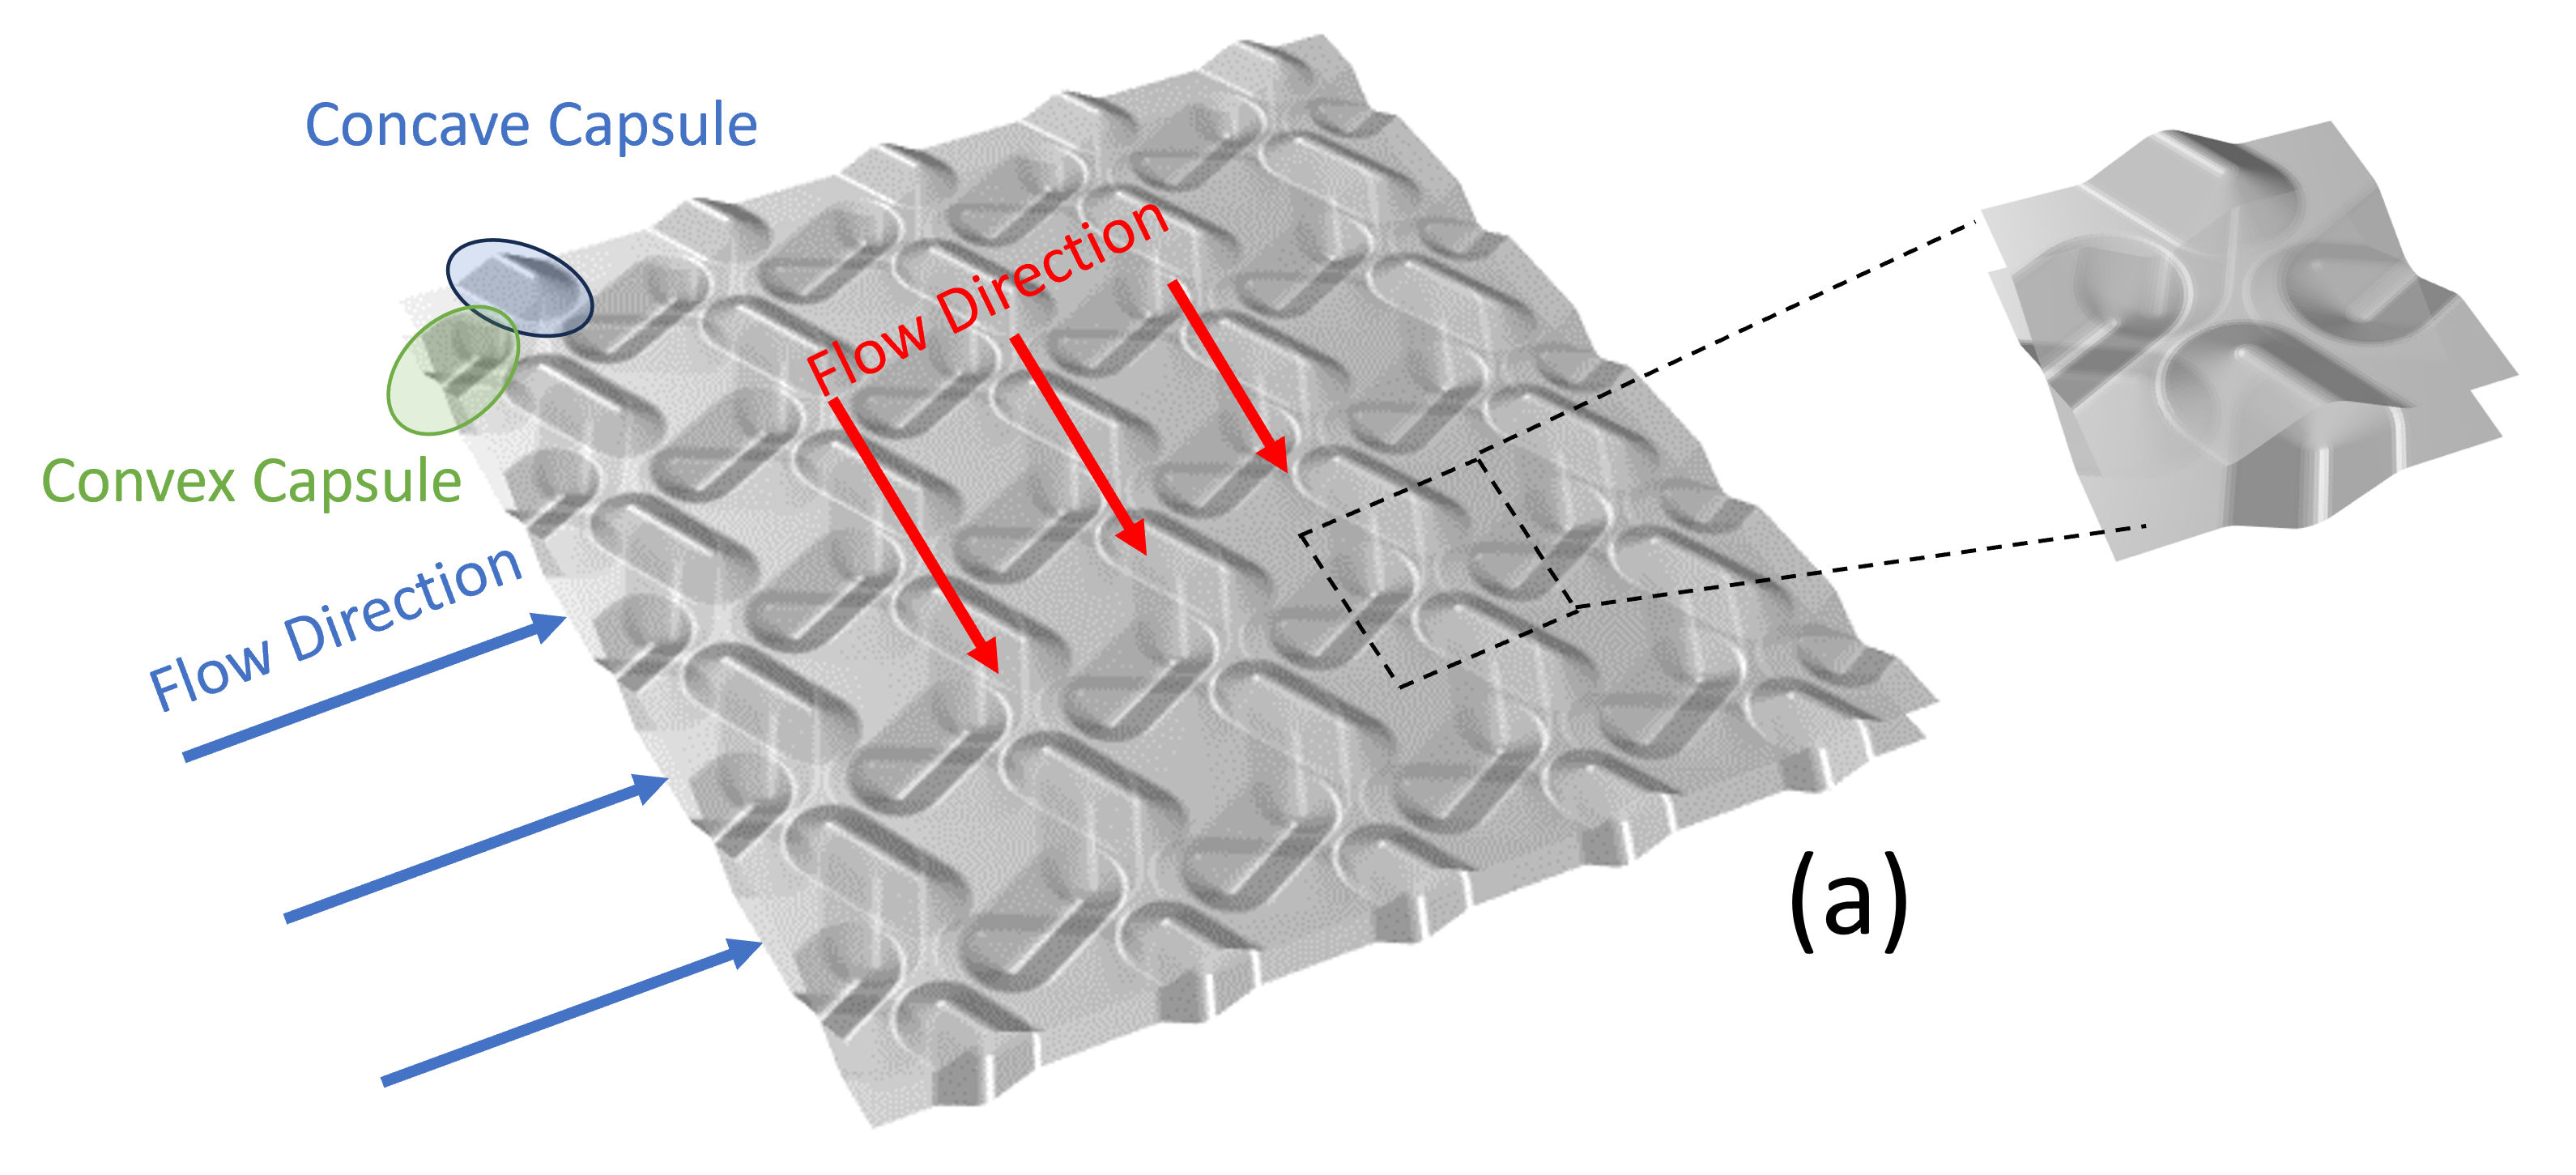
\includegraphics[width=0.48\textwidth]{media/image5_v3.png} &
    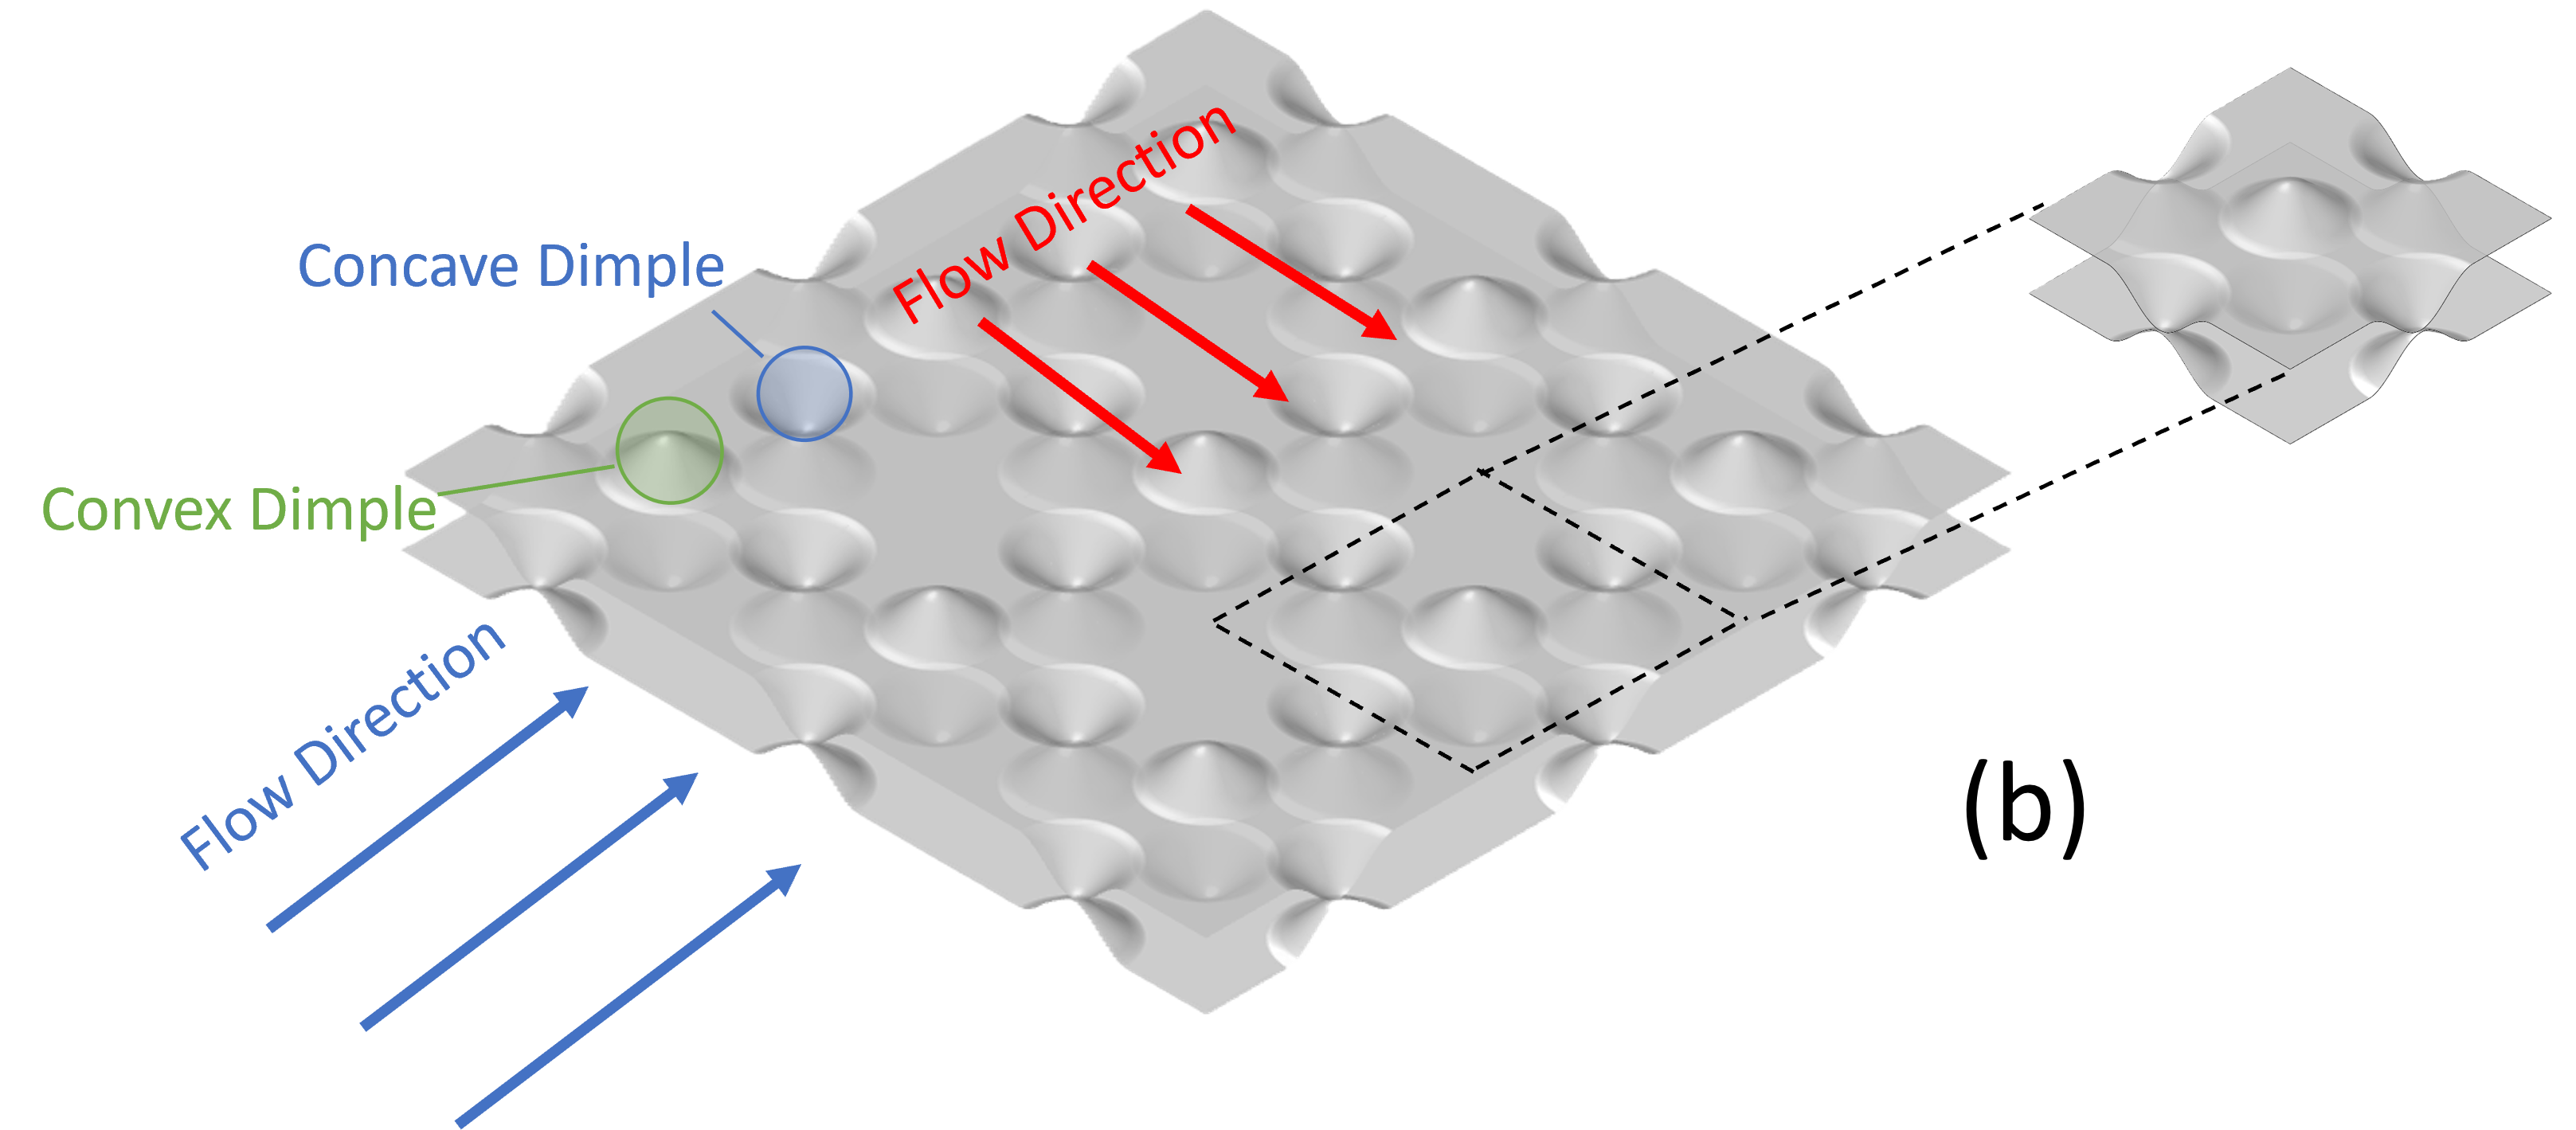
\includegraphics[width=0.48\textwidth]{media/image8_v4.png}\\
  \end{tabular}
  \par\smallskip
  % Editable boundary annotations over a mesh-derived PNG; no new figure number.
\begin{tikzpicture}[font=\footnotesize]
  \node[anchor=south west,inner sep=0] (mesh) at (0,0)
    {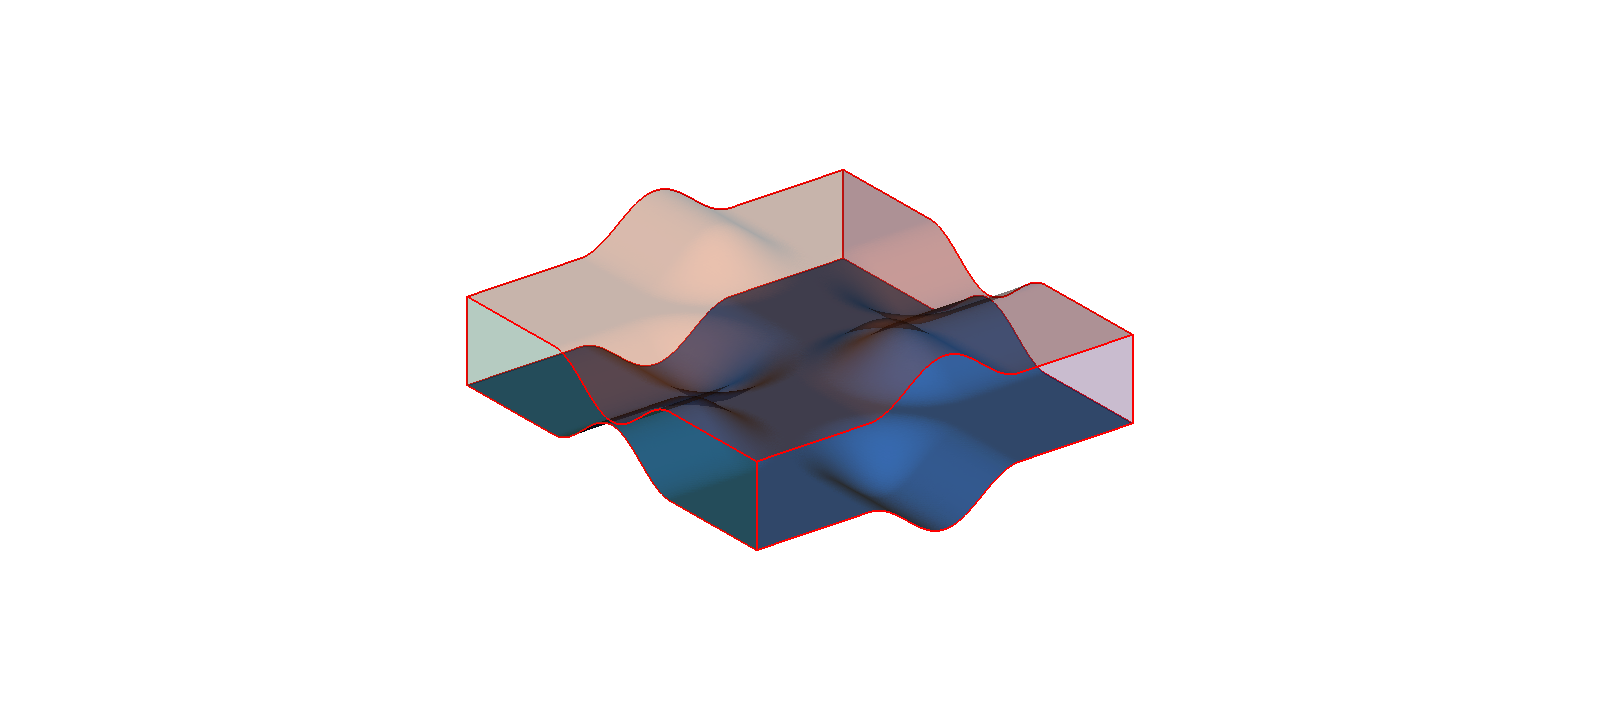
\includegraphics[width=0.96\linewidth]{media/BoundaryMap_CA0.png}};
  \begin{scope}[x={(mesh.south east)},y={(mesh.north west)}]
    \tikzset{labelbox/.style={fill=white,fill opacity=0.95,text opacity=1,align=center,inner sep=2pt},
             pointer/.style={->,line width=0.55pt}}
    \node[anchor=west] at (0.03,0.91) {\textbf{(c)} $\theta_c = 0^o$ boundary map};
    \node[labelbox,text=blue!70!black] (w1) at (0.80,0.17) {\texttt{wall\_1}: lower\\$T_w=333$ K};
    \draw[pointer,blue!70!black] (w1.west) -- (0.53,0.30);
    \node[labelbox,text=orange!70!black] (w2) at (0.66,0.88) {\texttt{wall\_2}: upper\\$T_w=333$ K};
    \draw[pointer,orange!70!black] (w2.south) -- (0.50,0.64);
    \node[labelbox,text=green!40!black] (in) at (0.15,0.41) {\texttt{inlet}\\$x=-12.5$ mm\\$T_{in}=293$ K};
    \draw[pointer,green!40!black] (in.east) -- (0.36,0.44);
    \node[labelbox,text=violet] (out) at (0.84,0.61) {\texttt{outlet}\\$x=+12.5$ mm\\$p_g=0$ Pa};
    \draw[pointer,violet] (out.west) -- (0.65,0.53);
    \node[labelbox] (p1) at (0.39,0.14) {\texttt{span\_top}\\$y=-12.5$ mm};
    \draw[pointer] (p1.north) -- (0.55,0.33);
    \node[labelbox] (p2) at (0.30,0.85) {\texttt{span\_bot}\\$y=+12.5$ mm};
    \draw[pointer] (p2.south) -- (0.45,0.68);
    \node[labelbox] at (0.55,0.48) {Water passage};
    \node[align=center] at (0.53,0.015) {Lateral faces: periodic pair; walls: no-slip};
  \end{scope}
\end{tikzpicture}

  \caption{Schematics and unit cells for (a) a capsule-type plate heat exchanger (CPHE) and (b) a dimple-type plate heat exchanger (DPHE); blue and green labels in these panels denote concave and convex embossings. (c) Boundary map from the $\theta_c$ 0\degree mesh. Blue and orange identify the lower and upper heated walls; water occupies the gap. The green inlet and purple outlet are distinguished from the lateral periodic pair. Colours identify regions, not temperature. The model contains no solid plate volume or separate exterior-air region.}
  \label{figure2}
\end{figure}

\begin{table}[H]
\centering
\caption{Dimensions of the initial geometry}
\label{tab:dim-initial}
\renewcommand{\arraystretch}{1.3}
\begin{tabular}{lcccccc}
\hline
\textbf{Type} & $l$ (mm) & $w$ or $D$ (mm) & $l_c$ or $l_d$ (mm) & $h_c$ or $h_d$(mm) & $\theta_c$ or $\theta_d$ (deg) \\
\hline
CPHE & 20 & 10 & 25 & 2 & 0\degree \\
\hline
DPHE &  & 10 & 25 & 2 & 0\degree \\
\hline
\end{tabular}
\end{table}

\subsubsection{CPHE}
\label{sec:cphe_geometry}

Figure~\ref{figure2} shows the CPHE channel formed between two capsule-embossed plates. Consecutive plates are inverted and rotated, so alternating concave and convex embossings form the spiral-like pattern of two concave and two convex capsules shown in Figure~\ref{figure1}. The geometric parameters are capsule length ($l$), width ($w$), height ($h_c$), unit-cell length ($l_c$), angle ($\theta_c$), and centre $C$, defined by the intersection of perpendicular lines through the capsule midpoints. The angle $\theta_c$ is measured anticlockwise from the mainstream flow direction to the capsule major axis; at $0\degree$, they are aligned. Higher angles rotate the capsule CAD anticlockwise while the flow-entry direction remains fixed normal to the inlet, with $l$, $w$, $h_c$, and $l_c$ unchanged. Table~\ref{tab:dim-initial} lists the initial dimensions.

\subsubsection{DPHE}
\label{sec:dphe_geometry}

Figure~\ref{figure2} shows the DPHE channel and unit cell formed by plates with opposing dimple embossings. The same unit-cell approach is used, with dimple height ($h_d$), diameter ($D$), and unit-cell length ($l_d$) as the main dimensions. Because each dimple is circular, the CAD geometry remains fixed during the angle sweep. The flow-entry angle $\theta_d$ is measured from the fixed line joining adjacent dimple centres to the mainstream flow direction (Figure~\ref{figure1}) and is varied by changing the direction from which flow enters the unchanged dimple array. Table~\ref{tab:dim-initial} lists the initial dimensions.

\subsubsection{Boundary conditions and computational workflow}
\label{sec:periodic_boundary}

The lateral faces form a translational periodic pair. In the streamwise direction, an external \emph{quasi-periodic iteration loop} transfers the outlet Cartesian velocity components, turbulent kinetic energy $k$ and specific dissipation rate $\omega$ to the inlet for the next period; the inlet and outlet are not a built-in periodic boundary pair. One period comprises the steady solver iterations between successive profile transfers. The inlet temperature remains 293~K and no outlet temperature profile is imposed at the inlet. Both no-slip walls are held at 333~K. The pressure outlet has zero gauge pressure; its 293.7~K total-temperature setting applies only to fluid entering through that boundary during local backflow.

With constant fluid properties and no buoyancy coupling, the momentum and turbulence solution is independent of temperature. The streamwise loop therefore targets a repeatable hydrodynamic state, but neither the block count nor a stable heat-transfer integral establishes thermal periodicity. The thermal results are interpreted as unit-cell heating with quasi-periodic hydrodynamic profile transfer, not as a demonstrated thermally fully developed periodic solution. The workflow below describes the calculation structure.

Figure~\ref{figure2}(c) locates the boundaries on an example computational domain, and Table~\ref{tab:bc-settings} summarizes the recovered settings. The two walls are opposing wetted surfaces of one water passage, not the inner and outer faces of a meshed solid plate. The coefficient reporting reference is assigned as $T_{\mathrm{ref}}=T_{f,ave}$ for each saved solution, as defined in Equation~\eqref{eq:h_ave} and its accompanying fluid-domain mass-average temperature definition; it is not an additional imposed fluid boundary temperature.

\paragraph{Calculation and Testing Sequence}
Scheme~\ref{scheme:simulation-workflow} summarizes the following sequence for each parameter case.
\begin{enumerate}
  \item \textbf{Construct the domain and mesh.} Select the case from Table~\ref{tab:geom_cases}, varying only the nominated angle or height while retaining the companion parameters. Construct the capsule geometry, or retain the dimple array and change the flow-entry direction for its angle sweep. Generate the fluid-domain poly-hexacore mesh with near-wall prism layers and the mesh-quality controls in Section~\ref{sec:mesh}. Identify the inlet, outlet, two heated walls and lateral periodic pair. Evaluate $A_0$, $S_1$, $S_2$ and $D_e$, then calculate the reference speed for $\mathrm{Re}=4282$.
  \item \textbf{Assign models and solve a period.} Apply the constant water properties, energy equation, SST $k$--$\omega$ model, coupled pressure--velocity scheme and second-order discretization listed in Table~\ref{tab:bc-settings}. Starting from the current inlet data, iterate the steady equations and check the configured residual targets. Velocity, mass-flow, pressure-drop and thermal-report trends provide separate checks on physical-output stability; low residuals alone are insufficient.
  \item \textbf{Transfer the outlet profiles.} At the end of one period, export the outlet velocity components, $k$ and $\omega$, map them to the inlet, and apply the saved profile-scaling expressions before the next period. The velocity field is scaled to the reference mean speed and its in-plane direction is corrected to the prescribed flow-entry direction. The velocity scale factor is denoted as $a$, the inlet velocity component $u_x$, $u_y$, $u_z$, and $\omega$ will be scaled by $a$, while $k$ will be scaled by $a^2$. Keep $T_{in}=293$~K and the wall temperatures unchanged. Compare available profile and integral-output records between periods to assess hydrodynamic repeatability.
  \item \textbf{Reduce the final fields consistently.} Batch post-processing extracts the mesh areas, area-averaged inlet/outlet pressures, separate wall heat rates and fluid-domain mass-average static temperature from the saved case/data pairs. The same expressions in Section~\ref{sec:numerical_methods} give $D_e$, $u$, $h_{ave}$, Nu and $f_F$; Equations~\eqref{eq:PEC} and~\eqref{eq:red} give PEC and RED. Signed mass and enthalpy fluxes supply separate conservation checks. Store outputs by case label, retain the geometric and flow-direction identifiers, and compare the four sweeps and the targeted combined dimple case. This automated data-reduction step does not imply that the original geometry generation and solver loop were fully automated.
\end{enumerate}

\begin{scheme}[H]
\centering
\begin{tikzpicture}[
  font=\small,
  process/.style={draw=black!65,rounded corners=2pt,fill=black!3,
    text width=6.9cm,align=center,inner sep=6pt,minimum height=1.0cm},
  check/.style={diamond,draw=black!65,fill=black!3,aspect=3.2,
    text width=4.0cm,align=center,inner sep=1pt},
  transfer/.style={draw=black!65,rounded corners=2pt,fill=blue!5,
    text width=3.0cm,align=center,inner sep=6pt},
  arrow/.style={-{Stealth[length=2.2mm]},semithick,draw=black!75},
  edgeword/.style={font=\footnotesize,fill=white,inner sep=2pt}
]
  \node[process] (prepare) at (0,0)
    {Select parameter case; construct fluid domain\\
     Mesh with prism layers; check zones and quality};
  \node[process,below=5mm of prepare] (setup)
    {Set $D_e$ and $u$ for $\mathrm{Re}=4282$; apply models\\
     Lateral periodic pair; $T_{in}=293$~K, $T_w=333$~K};
  \node[process,below=5mm of setup] (solve)
    {Steady solver iterations within one period $n$\\
     Use current inlet velocity, $k$ and $\omega$ profiles};
  \node[check,below=5mm of solve] (residual)
    {Configured residual\\targets met?};
  \node[process,below=5mm of residual] (monitor)
    {Inspect $h_{ave}$, $\Delta p$, $\Delta k$,and $\Delta \omega$ \\
     *$\Delta p$, $\Delta k$,and $\Delta \omega$ between inlet and outlet};
  \node[check,below=5mm of monitor] (blocks)
    {Are all the monitored parameters monotonic or oscillatory converged?};
  \node[transfer,right=9mm of blocks] (map)
    {Export profiles\\from outlet\\
     Map and scale\\$\mathbf{u}$, $k$, $\omega$ at inlet\\
     Keep $T_{in}=293$~K\\
     Next Period};
  \node[process,below=5mm of blocks] (reduce)
    {Save final fields and monitor records\\
     Batch reduction: $Q_1,Q_2,T_{f,ave},h_{ave},\mathrm{Nu},f_F$};
  \node[process,below=5mm of reduce] (compare)
    {Repeat for remaining parameter cases\\
     Compare Nu, $f_F$, PEC and RED on the same basis};

  \draw[arrow] (prepare) -- (setup);
  \draw[arrow] (setup) -- (solve);
  \draw[arrow] (solve) -- (residual);
  \draw[arrow] (residual.west) -- ++(-8mm,0) |- (solve.west)
    node[edgeword,pos=0.22,left] {No: continue};
  \draw[arrow] (residual) -- node[edgeword,right] {Yes} (monitor);
  \draw[arrow] (monitor) -- (blocks);
  \draw[arrow] (blocks.east) -- node[edgeword,above] {Yes} (map.west);
  \draw[arrow] (map.north) |- (solve.east);
  \draw[arrow] (blocks) -- node[edgeword,right] {No} (reduce);
  \draw[arrow] (reduce) -- (compare);
\end{tikzpicture}
\caption{Computational workflow and streamwise quasi-periodic iteration loop. Steady solver iterations are nested inside the reported profile-transfer sequence; the lateral periodic pair remains active throughout. Temperature is not transferred from outlet to inlet. Physical-output stability is assessed separately from the period count. The final batch-reduction stage refers to the revised post-processing of the saved solutions.}
\label{scheme:simulation-workflow}
\end{scheme}
\clearpage


\begingroup
\small
\renewcommand{\arraystretch}{1.15}
\begin{longtable}{@{}p{0.25\textwidth}p{0.71\textwidth}@{}}
\caption{Boundary conditions, varied parameters and numerical settings recovered from the saved cases. Reporting quantities are distinguished from physical boundary conditions.}
\label{tab:bc-settings}\\
\hline
\textbf{Item} & \textbf{Setting / interpretation}\\
\hline
\endfirsthead
\caption[]{(continued)}\\
\hline
\textbf{Item} & \textbf{Setting / interpretation}\\
\hline
\endhead
\hline
\endfoot
Solver / formulation & Ansys Fluent 2024 R1 (saved case/data provenance); three-dimensional, double-precision, steady, single-phase, pressure-based RANS.\\
Physical domain & One liquid-water fluid cell zone between two heated walls. No meshed solid plate or separate exterior-air domain; no conjugate solid conduction is solved.\\
Fluid properties & Constant $\rho=998.2$~kg/m$^3$, $\mu=0.001003$~Pa\,s, $C_p=4182$~J/(kg\,K), $\lambda=0.6$~W/(m\,K).\\
Turbulence / energy & SST $k$--$\omega$ model; energy equation enabled.\\
Inlet (\texttt{inlet}) & Velocity inlet at $x=-L/2$. Mapped outlet Cartesian velocity components, $k$ and $\omega$ are prescribed through the saved scaling expressions in the streamwise quasi-periodic iteration loop; $\mathrm{Re}=4282$ and $u=4282\mu/(\rho D_e)$. Uniform thermal inlet condition $T_{in}=293$~K; the outlet temperature profile is not reapplied.\\
Outlet (\texttt{outlet}) & Pressure outlet at $x=+L/2$; gauge pressure 0~Pa. \\
Lower and Upper heated wall & Stationary, no-slip, zero roughness height, fixed $T_w=333$~K. In the $\theta_c = 0^o$ example this is the wetted surface.\\
Lateral boundaries & Translational periodic pair in the $y$ direction. In the figure~\ref{figure2}(c) example, \texttt{span\_top} is at $y=-12.5$~mm and \texttt{span\_bot} at $y=+12.5$~mm; these are not heated walls.\\
Cell length / diameter & $L=25$~mm for every case.\\
Varied parameters & Four seven-case sweeps: $\theta_c,\theta_d=0$--$45\degree$ in $7.5\degree$ steps; $h_c,h_d=2$--$5$~mm in 0.5~mm steps. Fixed companion parameters and the combined dimple case are listed in Table~\ref{tab:geom_cases}.\\
Pressure--velocity coupling & Coupled pressure-based scheme with automatic global pseudo-time stepping for steady convergence.\\
Spatial discretization & Second-order pressure; second-order upwind momentum, energy, $k$ and $\omega$.\\
Configured residual criteria & $10^{-4}$ for continuity, momentum, $k$ and $\omega$; $10^{-6}$ for energy in all 29 labelled entries. \\
Streamwise quasi-periodic loop & Twenty calculation blocks per model, with outlet-to-inlet profile transfer between blocks (Scheme~\ref{scheme:simulation-workflow}). The block count is not an independent convergence measure.\\
PEC reporting surfaces / reference & Both heated walls; area-weighted built-in coefficient with case-specific $T_{\mathrm{ref}}=T_{f,ave}$, the mass-weighted volume average of static temperature over the entire fluid domain. For $\theta_c=0\degree$: 296.1537~K. Reporting normalization only; physical boundary temperatures are unchanged.\\
\end{longtable}
\endgroup


\subsubsection{Geometric parameters}
\label{sec:geometric_parameters}

A one-factor-at-a-time analysis is used to isolate the effects of capsule angle, capsule height, dimple height, and dimple flow-entry angle. Table~\ref{tab:geom_cases} summarizes the four seven-case sweeps, the fixed variables in each sweep, and the targeted combined dimple case. The tested ranges follow prior studies and commercially available products \citep{hamedi2024, jiang2019, jiang2019a, jiang2020, soman2019, mocnik2024, jing2019, Alfalaval2022}. The common physical models and case-specific residual targets are listed in Table~\ref{tab:bc-settings}. The recorded thermo-fluid outputs include Nu, $f$, $\Delta p$, and turbulence kinetic energy fields.

After the one-factor sweeps, one interaction case combines $\theta_d=45\degree$ with $h_d=5.0$~mm. It is reported separately from the two seven-case dimple sweeps. The same physical models, discretization choices and post-processing definitions are applied across the parameter matrix; the case-specific hydraulic diameter and reference speed are recalculated rather than imposing one common velocity. The four sweeps and combined case give 29 case labels but 27 distinct saved solutions, because two reference solutions are shared between sweeps. The combined case is an angle--height combination within the dimple family, not a capsule--dimple hybrid surface or a full factorial search.

\subsubsection{Performance evaluation criteria}
\label{sec:performance_criteria}

The following performance metrics are used to compare the results:

\begin{itemize}
  \item \textbf{Nusselt Number} (Nu): Measures convective heat transfer relative to conduction across the fluid layer. Higher Nu indicates stronger convective heat transfer.

  \item \textbf{Friction Factor} ($f$): Measures flow resistance from the simulated pressure loss, as defined by Equation~\eqref{eq:f}.

  \item \textbf{Performance Evaluation Criterion} (PEC): Combines heat transfer and flow resistance to rank all 29 cases on a common scale:
  \begin{equation}
  \mathrm{PEC} = \frac{\mathrm{Nu}}{f_F^{1/3}}
  \label{eq:PEC}
  \end{equation}
  Thermal--hydraulic assessment combines heat-transfer and pressure-loss measures \citep{thulukkanam2013,hamedi2024,jiang2019,jiang2020}. Equation~\eqref{eq:PEC} defines the \emph{unnormalized} index adopted in this study: higher values indicate a higher two-wall, fluid-temperature-referenced Nu relative to the cube root of $f_F$ on the same comparison basis. It is not a baseline-normalized enhancement factor or, by itself, proof of superior exchanger performance at equal pumping power. Its use here requires the same coefficient, temperature-reference convention and friction convention for every plotted case.
  Sections~\ref{sec:disc_capsule_angle}--\ref{sec:disc_dimple_angle} analyze trends in Nu and $f$ individually; section~\ref{sec:tgg_comparison} uses PEC to rank all cases and compare both embossing families.
\end{itemize}

The comparison identifies heat-transfer and flow-resistance trade-offs among the examined cases. Because each primary sweep changes one geometric variable while the others remain fixed and only one targeted combined case is included, the results do not establish a global optimum across interacting variables or untested conditions.

\paragraph{Relative Embossing Depth (RED)}
Embossing depth constrains plate spacing and channel size. Relative Embossing Depth (RED) is introduced to compare the protrusion height with the effective channel scale:
\begin{equation}
\text{RED} = \frac{h}{D_e}
\label{eq:red}
\end{equation}
where $h$ is the embossing height ($h_c$ or $h_d$) and $D_e$ is given by Equation~\eqref{eq:De}, with both lengths expressed in the same units. RED is a dimensionless descriptor defined for the present comparison, not an externally fitted correlation. It varies with height and, for the capsule-angle cases, with the measured mesh-dependent $D_e$. All dimple-angle cases share the same geometry and RED. Thus RED alone does not identify a unique geometric or flow-entry-angle case, even within the dimple-angle family.

\begin{table}[H]
\centering
\caption{Geometric parameter cases for CPHE and DPHE}
\label{tab:geom_cases}
\footnotesize
\renewcommand{\arraystretch}{1}
\begin{tabularx}{\textwidth}{ll>{\raggedright\arraybackslash}l>{\raggedright\arraybackslash}X}
\hline
\textbf{Heat Exchanger Type} & \textbf{Parameter} & \textbf{Cases} & \textbf{Description} \\ \hline
\multirow{2}{*}{CPHE (Capsule-Type)} 
& Capsule Angle ($\theta_c$) & 0\degree\ to 45\degree & Orientation of capsule pattern relative to main flow direction with 7.5\degree\ increments and a capsule height of 2.5~mm. \\
& Capsule Height ($h_c$) & 2--5~mm & Height of capsule embossing feature with 0.5~mm increments and a capsule angle of 22.5\degree. \\ \hline
\multirow{3}{*}{DPHE (Dimple-Type)} 
& Dimple Height ($h_d$) & 2--5~mm & Height of the dimple embossing feature with 0.5~mm increments and a dimple angle of 0\degree. \\
& Dimple Angle ($\theta_d$) & 0\degree\ to 45\degree & Angle between the main flow direction and the dimple pattern, varied in 7.5\degree\ increments with a dimple height of 3.5~mm. \\
& Combined Dimple Case & $\theta_d=45\degree$, $h_d=5.0$~mm & Targeted interaction case combining the highest-PEC dimple orientation with the maximum tested dimple height. \\ \hline
\end{tabularx}
\end{table}

\subsection{Mesh independence}
\label{sec:mesh}

An unstructured poly-hexacore mesh type is adopted for the mesh generation. With guidance from literature, certain criteria are set for the mesh generated to minimize discretizations and interpolation error \citep{sorgente2023, juretic2010}, including mesh orthogonality and mesh skewness. For this study, the criteria of minimum mesh orthogonality of 0.1 and maximum mesh skewness of 0.8 are set for all cases. Representative CPHE and DPHE meshes are shown in Figure~\ref{figure3}(a,b).

To accurately predict the wall heat transfer coefficient and the wall shear stress close to the wall, prism layers are included in the mesh generation. Prism layers are hexahedral cells that are normal to the wall boundary to capture the steep normal gradient in the mean velocity and temperature inside the thermal and hydraulic boundary layers. The total prism layer thickness should capture the turbulent boundary layer of the flow. The initial estimation of the total boundary layer thickness $\delta$ can be estimated through the following equation: $\delta/x = 0.16/\text{Re}_x^{1/7}$ \citep{cengel2014}, where $x$ is the total stream length, which is $l_c$ and $l_d$ for this study, and Re is the Reynolds number.

For the prism layers to accurately predict the near-wall behavior, the first prism layer thickness (or the first layer height) plays an important role in calculating the behavior at the viscous sub-layer, as it is related to $y^+$, which is a dimensionless distance normal to the wall, and the near-wall kinematic viscosity can be calculated accordingly.  o minimize the numerical uncertainty, $y^+$ <1 should be applied for the SST $k$--$\omega$ turbulence model \cite{eca2018}; the first layer height is set to 0.0002~mm, with 7 boundary layers and transition ratio as 0.5, the resultant $y^+$ is 0.087 (Figure~\ref{figure3}(a)).

A mesh-sensitivity study was performed for CPHE with $h = 2.5$~mm, as shown in Figure~\ref{figure3}(c). $f$ and Nu for five different meshes ranging from $\sim$100k to $\sim$1.1M elements are compared to determine the best coarsest mesh. The difference of $f$ and Nu between the results of $\sim$800k mesh count and $\sim$1.1M mesh count is less than 2.7\% and 2\%, respectively, on the original reporting basis; the $\sim$800k mesh was subsequently used. The historical Nu values in Figure~\ref{figure3}(c) have not been recalculated using the fluid-domain mass-average temperature, because the corresponding fields for all five mesh levels are unavailable in the present reconstruction. The quoted Nu difference therefore does not verify mesh independence of the revised thermal reporting definition.

\begin{figure}[!ht]
  \centering
  \begin{minipage}[b]{0.60\textwidth}
    \centering
    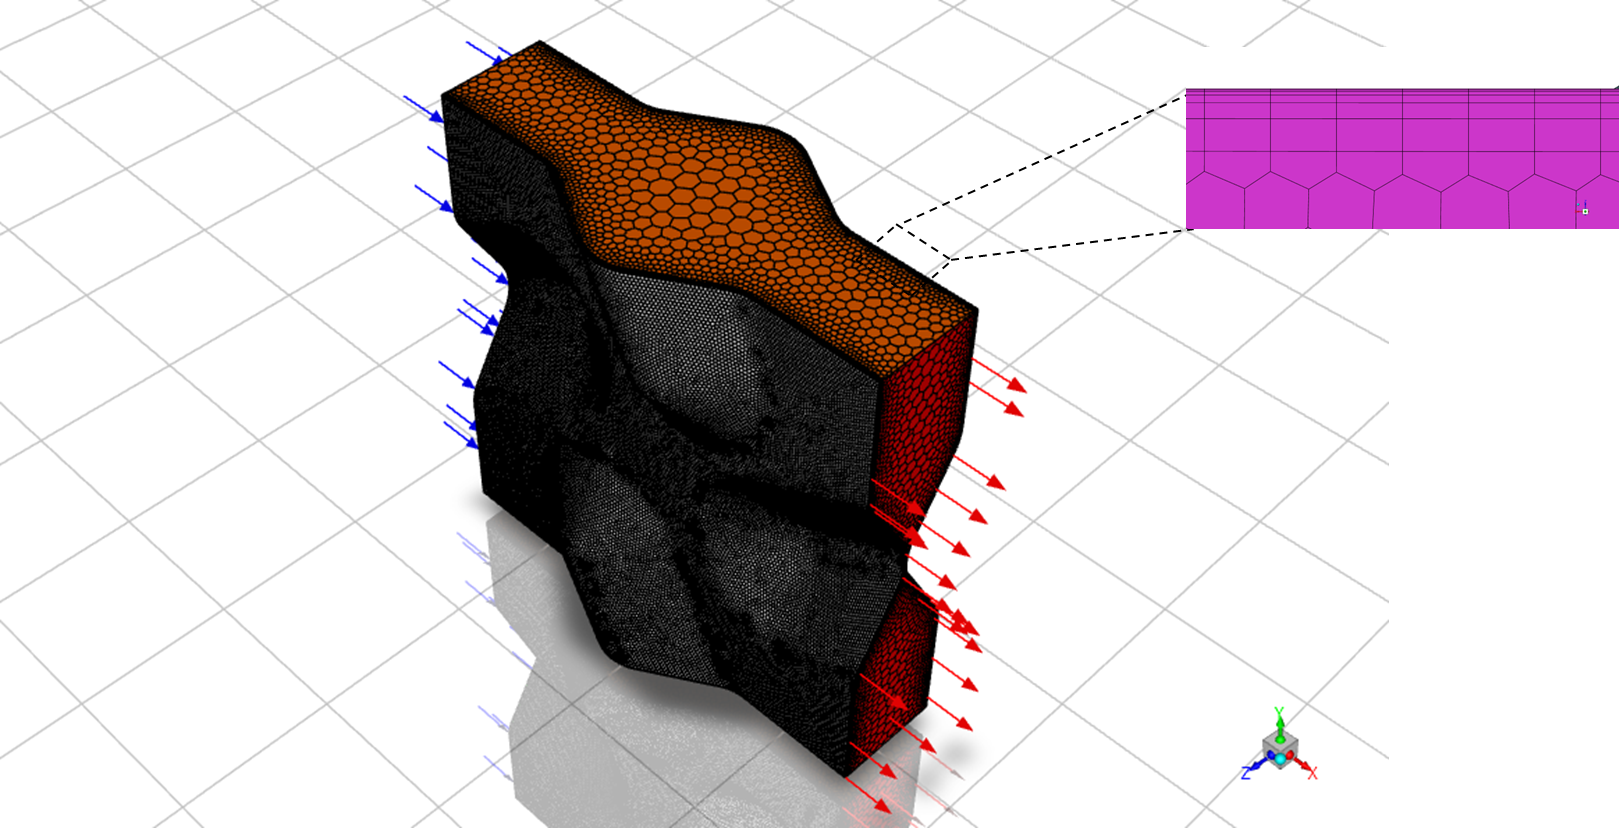
\includegraphics[width=\linewidth,height=4.8cm,keepaspectratio]{media/Picture4.png}\par
    \smallskip
    {\small (a) CPHE mesh and near-wall detail}
  \end{minipage}\hfill
  \begin{minipage}[b]{0.33\textwidth}
    \centering
    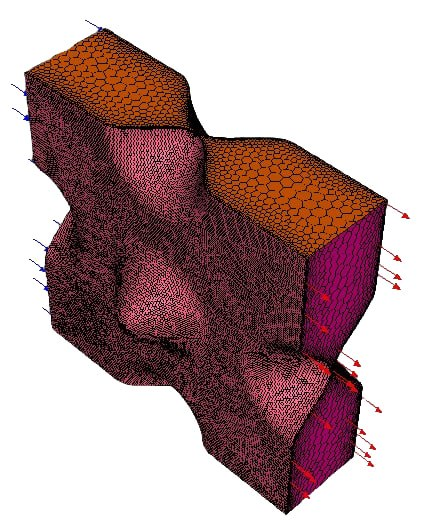
\includegraphics[width=\linewidth,height=4.8cm,keepaspectratio]{media/Figure3_DPHE_mesh.png}\par
    \smallskip
    {\small (b) DPHE mesh}
  \end{minipage}
  \par\medskip
  \begin{minipage}{0.66\textwidth}
    \centering
    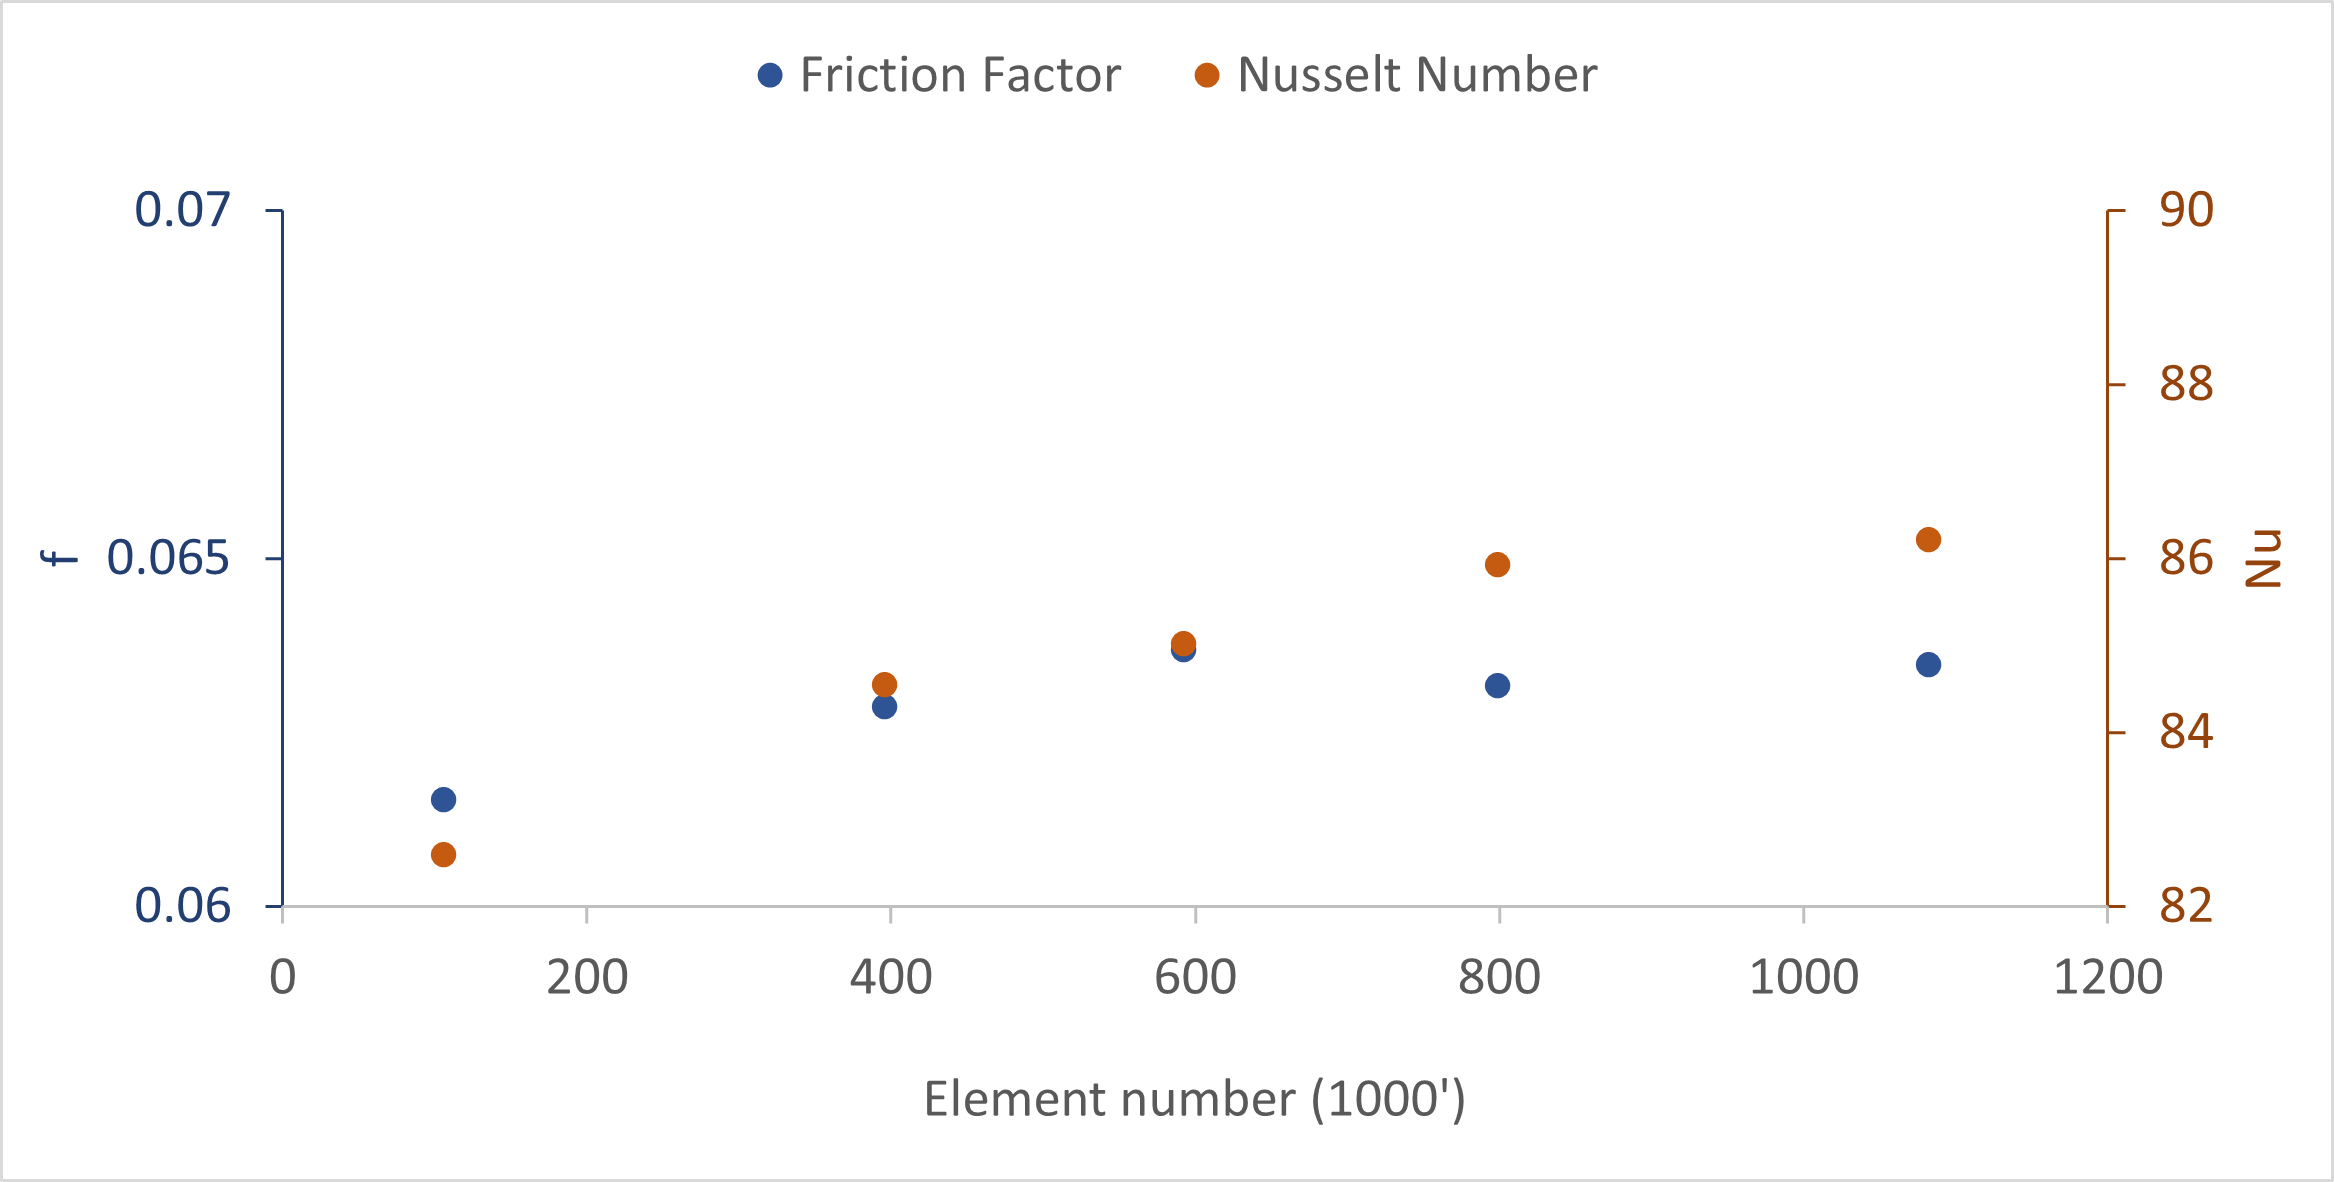
\includegraphics[width=\linewidth]{media/image10_v1.png}\par
    \smallskip
    {\small (c) CPHE mesh-sensitivity results}
  \end{minipage}
  \caption{Representative (a) CPHE and (b) DPHE meshes, and (c) CPHE mesh-sensitivity results.}
  \label{figure3}
\end{figure}

\paragraph{DPHE mesh-sensitivity assessment.}
A dedicated assessment was performed for a representative DPHE case using six meshes from 103k to 1622k cells (Table~\ref{tab:dphe_mesh_sensitivity}). The geometry, physical conditions and reporting basis were consistent across the meshes; iterative convergence, mesh consistency, direct velocity and fluid-temperature results, and near-wall resolution were verified before the comparison. Nu was evaluated using both heated walls and the fluid-domain mass-average reference temperature defined in Section~\ref{sec:numerical_methods}. Nu increased with refinement, whereas the Fanning friction factor approached a stable value on the two finest meshes. Refining from 855k to 1622k cells changed Nu and $f_F$ by 2.20\% and 0.095\%, respectively, relative to the finest-mesh values.

\begin{table}[!ht]
\caption{DPHE mesh-sensitivity results. The three finest meshes are used for the GCI assessment, with indices 1, 2 and 3 denoting fine, medium and coarse grids, respectively.}
\label{tab:dphe_mesh_sensitivity}
\centering
\begin{tabular}{rrrr}
\toprule
Cells ($10^3$) & Nu & $f_F$ & GCI grid index \\
\midrule
103 & 81.18688 & 0.065464 & --- \\
175 & 83.35945 & 0.066481 & --- \\
405 & 85.90751 & 0.068507 & --- \\
571 & 88.03678 & 0.070067 & 3 (coarse) \\
855 & 88.58099 & 0.069083 & 2 (medium) \\
1622 & 90.57817 & 0.069149 & 1 (fine) \\
\bottomrule
\end{tabular}
\end{table}

Spatial discretization sensitivity in Nu was quantified using the grid convergence index (GCI) formulation of \citet{celik2008gci}. For a three-dimensional mesh, the representative grid spacing is
\[
h_g=\left[\frac{1}{N}\sum_{i=1}^{N}\Delta V_i\right]^{1/3}
=\left(\frac{V}{N}\right)^{1/3},
\]
where $V$ is the fluid-domain volume and $N$ is the number of cells; the solution variable is $\phi=\mathrm{Nu}$. For the common domain volume, $r_{21}=h_{g,2}/h_{g,1}=1.238$ and $r_{32}=h_{g,3}/h_{g,2}=1.144$. The unequal-ratio apparent-order calculation gives $p=3.269$. With a safety factor of 1.25,
\[
e_a^{21}=\left|\frac{\phi_1-\phi_2}{\phi_1}\right|,
\qquad
\mathrm{GCI}_{21}=\frac{1.25e_a^{21}}{r_{21}^{p}-1}\times100\%.
\]
The corresponding medium/coarse expressions use $e_a^{32}=|\phi_2-\phi_3|/|\phi_2|$ and $r_{32}$. The resulting values are $\mathrm{GCI}_{21}=2.73\%$ for the 1622k/855k pair and $\mathrm{GCI}_{32}=1.39\%$ for the 855k/571k pair, referenced to the fine and medium grids, respectively. Both refinement ratios are below the recommended value of 1.3, and the two pairs do not establish a consistent asymptotic limit. The GCIs are therefore indicative estimates, not evidence that the medium mesh is more accurate than the fine mesh. The 855k-cell mesh was selected as a practical balance between computational cost and the observed sensitivity of Nu and $f_F$.



% Four-point D3-PA comparison: retain the author-supplied comparison data.
% Reference digitisation and comparison/numerical-verification checks remain
% distinct from the reported arithmetic agreement; do not infer a new area basis.
\subsection{Validation benchmark}
\label{sec:du-validation}

\noindent\textbf{Four-point experimental comparison.} The independent heat-transfer benchmark uses the D3 projected-area (PA) experimental series of \citet{du2025}. Four Nusselt numbers obtained with the present quasi-periodic inlet--outlet loop are compared with the experimental reference over the reported range $2089.966\leq\mathrm{Re}\leq6597.217$. This separate benchmark is not an additional member of the 29-case parameter matrix. Table~\ref{tab:du-validation-comparison} records the four numerical results, the corresponding supplied reference digitisation and the reported signed differences, providing a multi-point assessment of the predicted D3 heat-transfer response.

\paragraph{Experimental benchmark and data provenance.}
Du et al. report a D3 pressing depth of 2.0~mm, dimple pitch of 7.6~mm and dimple size of 2.0~mm, with a $90\degree$ layout and 0.25~mm plate thickness (their Table~3). The water--water experiment used vertical counterflow with cold- and hot-side inlet temperatures of 50 and 70~$^\circ$C, respectively. The selected reference is the \emph{open blue triangle} D3-PA series in their Figure~4(b), not the filled D3 effective-area (EA) markers, their fitted correlation, or their separate D1 numerical-validation results. PA and EA denote two area-based reductions of the same D3 experiment, not different dimple geometries. The supplied reference points are digitised graph estimates rather than a published numerical data table. The comparisons below use the reference values reported in Table~\ref{tab:du-validation-comparison}.

Figure~\ref{fig:du-d3-geometry} shows the reconstructed D3 unit-cell fluid domain used for the benchmark, with its principal dimensions listed in Table~\ref{tab:du-d3-dimensions}. The supplied CAD has opposing cut planes separated by 7.60~mm in both in-plane directions and a nominal 2.00~mm central contact footprint. Its approximately 4.00~mm full vertical envelope describes both bounding walls and must not be interpreted as a uniform local channel gap or as the plate thickness. The 0.25~mm experimental plate thickness is reported for provenance only; no solid plate volume is included in this fluid-domain geometry.

% Dimensioned D3 geometry from the supplied, unmodified fluid-domain STEP.
% Panel arrangement and dimension table remain editable LaTeX.
\begin{figure}[H]
  \centering
  \begin{minipage}[t]{0.49\linewidth}
    \centering
    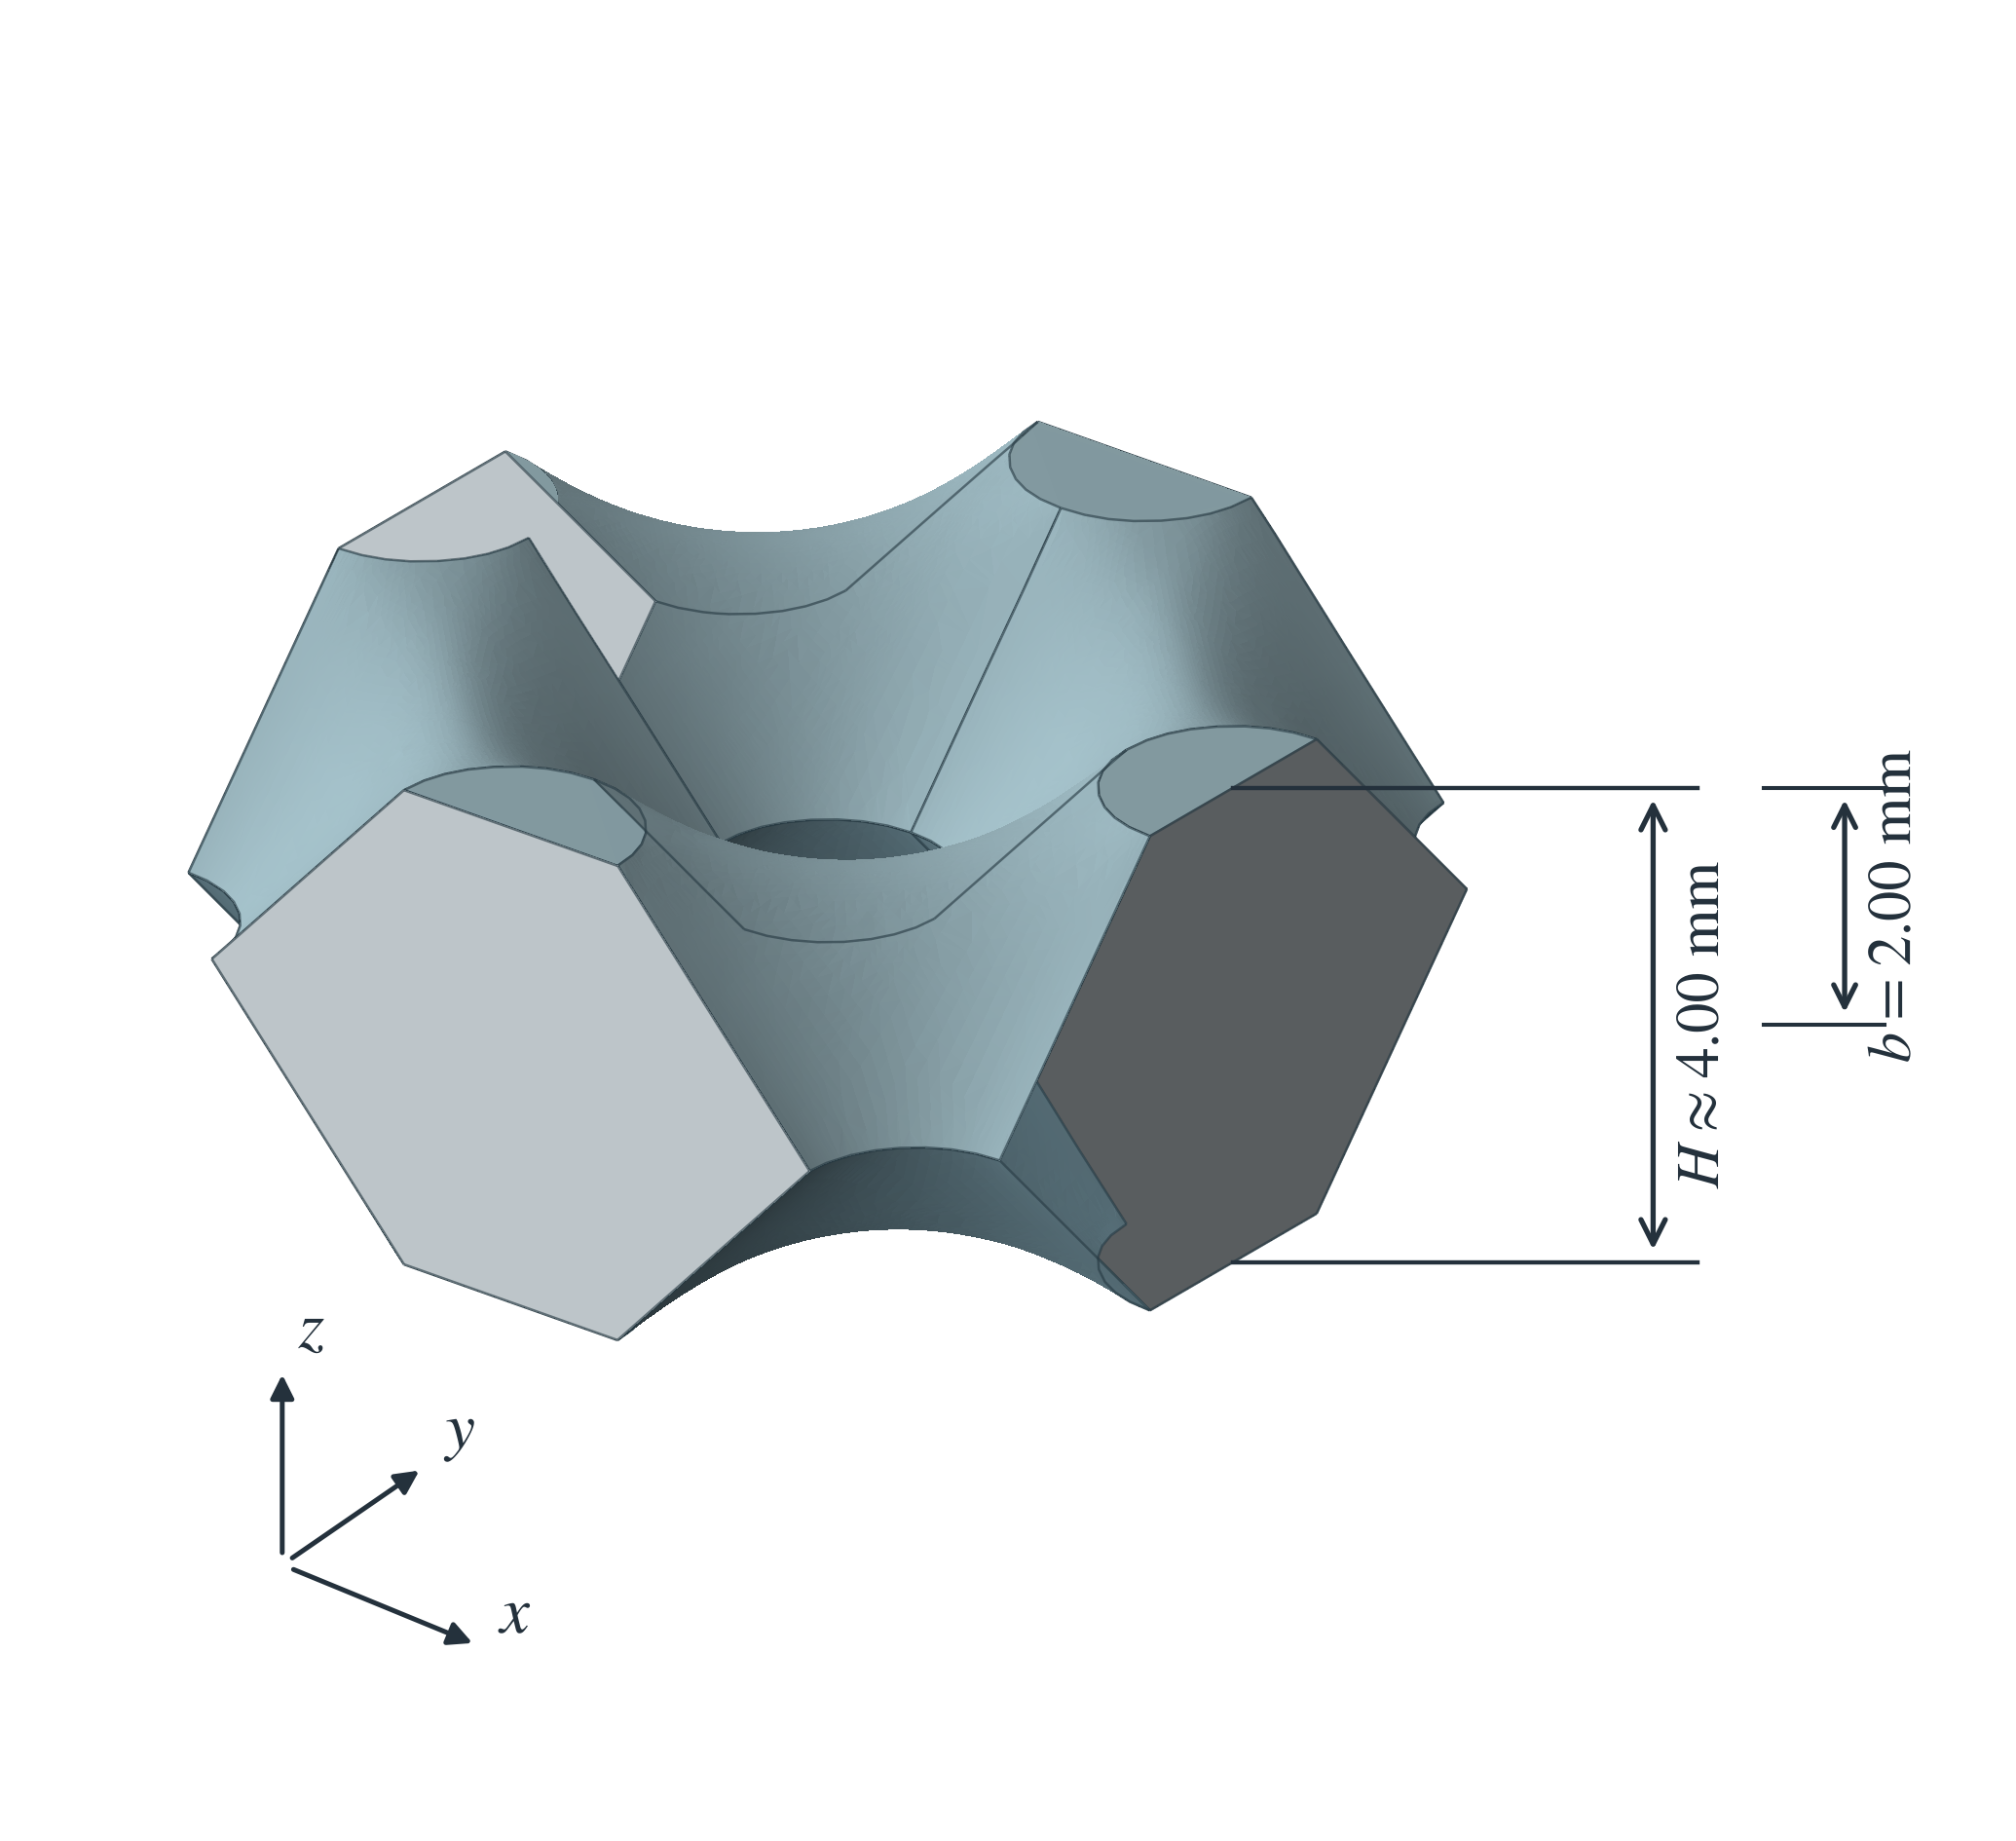
\includegraphics[width=\linewidth]{du_d3_geometry_iso.png}\par
    \small\textbf{(a)} Isometric fluid-domain view
  \end{minipage}\hfill
  \begin{minipage}[t]{0.49\linewidth}
    \centering
    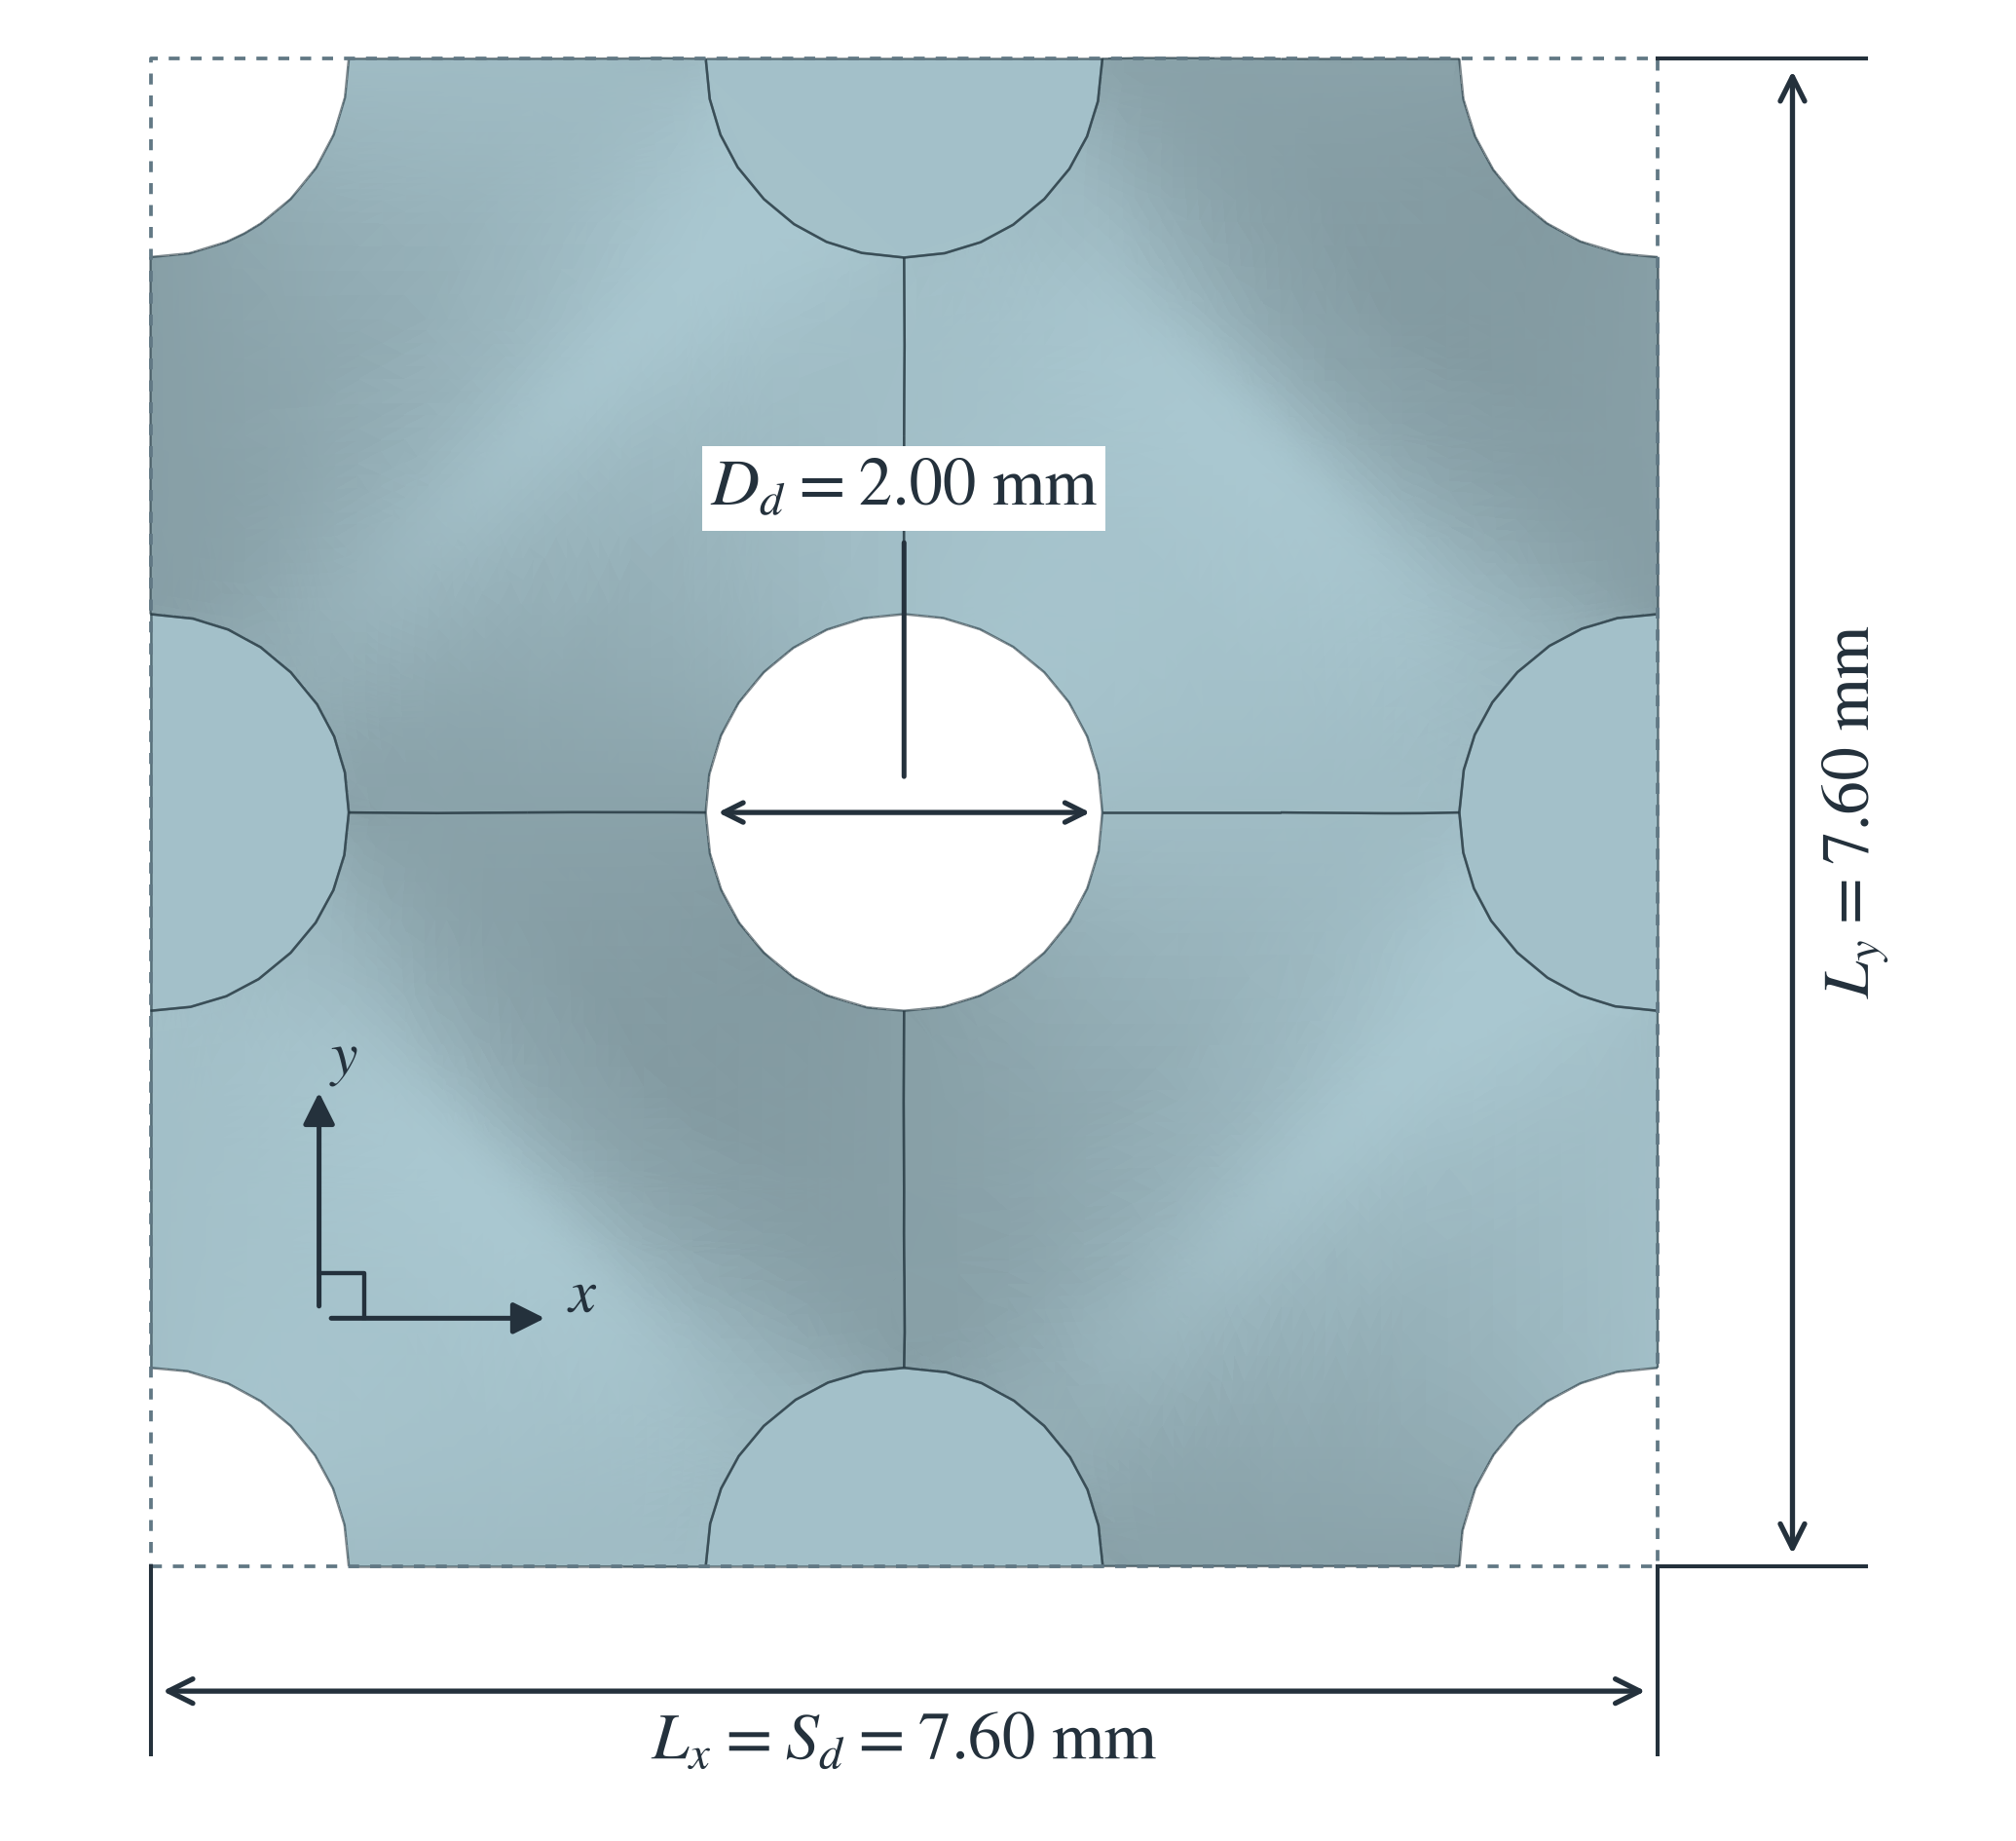
\includegraphics[width=\linewidth]{du_d3_geometry_plan.png}\par
    \small\textbf{(b)} Plan view and repeat dimensions
  \end{minipage}
  \caption{D3 validation unit cell visualised from the supplied CAD fluid domain: (a) isometric view with the nominal pressing depth $b$ and approximate full vertical envelope $H$; (b) plan view with repeat lengths $L_x$, $L_y$ and nominal dimple size $D_d$. Linear dimensions are in millimetres. $S_d$ is the reported dimple pitch. Colours distinguish geometric surfaces and are not solution fields; the central circular footprint is excluded from the fluid.}
  \label{fig:du-d3-geometry}
\end{figure}

\begin{table}[H]
  \centering
  \caption{Dimensions of the D3 benchmark geometry. Reported experimental dimensions follow \citet{du2025}, Table~3; CAD dimensions describe the supplied fluid-domain model. Nominal values are not manufacturing-tolerance or exact surface-matching claims.}
  \label{tab:du-d3-dimensions}
  \small
  \setlength{\tabcolsep}{4pt}
  \renewcommand{\arraystretch}{1.13}
  \begin{tabular}{@{}p{0.32\linewidth}cp{0.12\linewidth}p{0.39\linewidth}@{}}
    \hline
    \textbf{Quantity} & \textbf{Symbol} & \textbf{Value} & \textbf{Definition / source}\\
    \hline
    Unit-cell repeat lengths & $L_x,L_y$ & 7.60~mm & Opposing CAD cut-plane separations in $x$ and $y$.\\
    Dimple pitch & $S_d$ & 7.60~mm & Reported D3 pitch; matches the nominal cell repeat.\\
    Pressing depth & $b$ & 2.00~mm & Reported D3 pressing depth; nominal height from the contact plane to one wall extremum.\\
    Dimple size & $D_d$ & 2.00~mm & Reported D3 dimple size; central contact-footprint diameter in the plan view.\\
    Full vertical fluid envelope & $H$ & $\approx4.00$~mm & Approximate CAD span from $z\approx-2$ to $+2$~mm; not a uniform local channel gap.\\
    Dimple arrangement angle & $\beta$ & $90\degree$ & Reported D3 layout; distinct from the flow-entry angle.\\
    Solid plate thickness & $\delta_p$ & 0.25~mm & Reported experimental plate thickness.\\
    \hline
  \end{tabular}
\end{table}


Figure~\ref{fig:du-d3-mesh} shows the computational mesh of the D3 validation unit cell, comprising 894{,}592 cells.

% Author-supplied D3 mesh image and 894592-cell count, received 2026-10-05.
% The native 440 x 421 image is retained without resampling or content edits.
\begin{figure}[H]
  \centering
  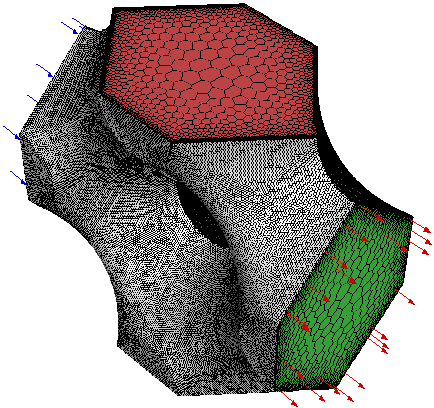
\includegraphics[width=0.38\linewidth]{du_d3_mesh.png}
  \caption{Computational mesh of the D3 validation unit cell, comprising 894{,}592 cells.}
  \label{fig:du-d3-mesh}
\end{figure}


\paragraph{Method-matched quasi-periodic calculation.}
The benchmark retains the steady, single-phase, pressure-based RANS formulation, SST $k$--$\omega$ closure and numerical scheme described in Sections~\ref{sec:numerical_methods} and~\ref{sec:periodic_boundary}. The lateral faces form a translational periodic pair. In the streamwise direction, the velocity inlet and pressure outlet remain separate boundaries: outlet Cartesian velocity components, $k$ and $\omega$ are mapped and scaled onto the inlet between calculation blocks using the existing quasi-periodic loop. The thermal treatment retains a fixed uniform inlet-temperature reset, prescribed isothermal heated walls and no outlet-to-inlet temperature-profile transfer. Hydrodynamic repeatability does not establish thermal periodicity.

The four benchmark points are at $\mathrm{Re}=2089.966$, $4234.524$, $6137.484$ and $6597.217$; the parametric sweeps remain at $\mathrm{Re}=4282$. For each benchmark point, the manuscript's reference-speed relation is
\[
 u=\frac{\mathrm{Re}\,\mu}{\rho D_e}.
\]
Here $D_e$ follows Equation~\eqref{eq:De}, using the D3 cell's own $A_0$, $L$ and both wetted wall areas, not the parametric geometries' 25~mm cell length. The profile-scaling speed $u$, actual inlet-normal bulk speed, net mass flow and mass flux must be distinguished and documented. Du et al. list $D_{\mathrm{hyd}}=4.0$~mm and $D_{\mathrm{eq}}=3.18$~mm and state that hydraulic diameter is used for their Reynolds and Nusselt numbers. 

\paragraph{Heat-transfer reduction and the PA comparison.}
The primary numerical definition remains Equation~\eqref{eq:h_ave}, using both wall heat rates and wetted areas with the fluid-domain mass-average temperature $T_{f,ave}$, followed by Equation~\eqref{eq:Nu}, $\mathrm{Nu}=h_{ave}D_e/\lambda$, where $\lambda$ is water thermal conductivity. Selecting Du's PA series does not change these parametric-study definitions. Du et al. infer their coefficient through exchanger heat-transfer/resistance reduction and evaluate properties at an inlet/outlet bulk-temperature mean. A separately reported PA-equivalent numerical coefficient therefore requires the cell's projected heated area and a stated driving-temperature, property and diameter basis.

\paragraph{Four-point heat-transfer comparison.}
In order of increasing Reynolds number, the present study gives $\mathrm{Nu}=52.75$, $86.38$, $108.14$ and $113.68$, compared with the digitised D3--PA experimental reference values $51.76$, $85.29$, $111.02$ and $116.38$, respectively. Both sets increase monotonically over the four operating points. The signed tabulated difference is defined as
\[
 \delta_{\mathrm{Nu}}=100\,
 \frac{\mathrm{Nu}_{\mathrm{study}}-\mathrm{Nu}_{\mathrm{Du,PA}}}
 {\mathrm{Nu}_{\mathrm{Du,PA}}}\,\%.
\]
The reported signed differences are $+1.92\%$, $+1.28\%$, $-2.60\%$ and $-2.32\%$, respectively. The numerical predictions therefore slightly overestimate the experimental reference at the two lower Reynolds numbers and underestimate it at the two higher Reynolds numbers. Across all four points, the maximum absolute reported difference is $2.60\%$ and the mean absolute reported difference is $2.03\%$.
\begin{table}[H]
\centering
\caption{Four-point comparison of the present quasi-periodic calculation with the provisional digitisation of the open blue D3-PA experimental triangles of \citet{du2025}, Figure~4(b).}
\label{tab:du-validation-comparison}
\small
\renewcommand{\arraystretch}{1.15}
\begin{tabular}{rrrr}
\hline
\textbf{Reported Re} & \textbf{Supplied Du--PA Nu} & \textbf{Present study Nu} & \textbf{$\delta_{\mathrm{Nu}}$ (\%)}\\
\hline
2089.966 & 51.76  & 52.75 & $1.92$\\
4234.524 & 85.29  & 86.38 & $1.28$\\
6137.484 & 111.02 & 108.14 & $-2.60$\\
6597.217 & 116.38 & 113.68 & $-2.32$\\
\hline
\end{tabular}
\end{table}

The D3--PA results of \citet{du2025} are experimentally derived Nusselt numbers and thus provide an independent physical benchmark for validating the present numerical method. Agreement between computed and experimental Nusselt numbers at corresponding Reynolds numbers constitutes validation evidence for the unit-cell heat-transfer predictions, rather than merely agreement between numerical models. The reported four-point agreement therefore supports the method's ability to reproduce both the measured heat-transfer level and its increase with Reynolds number over the sampled D3 range. This validation evidence is specific to the D3 heat-transfer response under the examined conditions.



\section{Results and Discussion}
\label{sec:results}
\label{sec:discussion}

The numerical simulations conducted in this study provide detailed insight into the thermo-hydraulic behavior of capsule-type and dimple-type plate heat exchangers under a variety of geometric configurations. By examining the influence of selected design parameters namely the capsule angle and height in CPHE, and the dimple height and angle of flow in DPHE the impact on flow structures, pressure drop, and heat transfer performance is assessed. Key fluid dynamic behaviors, including vortex generation, turbulence intensity, and recirculating flow patterns, are visualized through turbulence kinetic energy contours and streamline plots. Temperature distributions further reveal the relationship between geometric enhancements and thermal mixing. These findings enable the identification of design trends that balance improved heat transfer effectiveness with manageable pressure penalties, supporting the development of more efficient compact heat exchanger designs. Figure~\ref{figure4} provides an overview of the four parametric sweeps by comparing the friction factor and Nusselt number for capsule angle, capsule height, dimple height, and dimple angle. The following subsections relate these performance trends to the corresponding flow and temperature fields.

% Figure 4: merged Nu--f comparisons for the angle and height sweeps.
% The two source plots remain separate so the panel layout stays editable in LaTeX.
\begin{figure}[H]
    \centering
    \begingroup
    \newlength{\figfourpanelwidth}
    \setlength{\figfourpanelwidth}{0.485\linewidth}

    \newcommand{\figfourpanel}[3]{%
        \begin{tabular}[t]{@{}c@{}}
            \includegraphics[width=\figfourpanelwidth]{#1}\\[-1pt]
            {\sffamily\bfseries\fontsize{8.5}{9.5}\selectfont (#2) #3}
        \end{tabular}%
    }

    \begin{tabular}[c]{@{}c@{\hspace{0.02\linewidth}}c@{}}
        \figfourpanel{media/Figure4_angle_comparison.png}{a}{Angle sweeps, $\theta_c$ and $\theta_d$} &
        \figfourpanel{media/Figure4_height_comparison.png}{b}{Height sweeps, $h_c/l_c$ and $h_d/l_d$}
    \end{tabular}
    \endgroup
    \caption{Fanning friction factor $f_F$ (blue) and two-wall Nusselt number Nu (orange), referenced to each case's fluid-domain mass-average temperature, for the four parametric sweeps: (a) capsule-angle and dimple-angle sweeps and (b) normalized capsule-height and dimple-height sweeps. The combined dimple case is excluded from these one-factor sweeps and is shown separately in Figure~\ref{figure15}.}
    \label{figure4}
\end{figure}


\subsection{CPHE parametric study}
\label{sec:cphe_results}

The CPHE study varies capsule angle and height. All four sweeps use the same constructed values as the PEC analysis: Nu is based on both heated walls and the case-specific fluid-domain mass-average temperature, and $f_F$ is the Fanning friction factor. Re\,=\,4282 is maintained using the case-specific $D_e$ and a common cell length of 25~mm. The steady-state flow fields support interpretation of these trends; TKE alone does not quantify wall heat transfer.

\subsubsection{Capsule angle}
\label{sec:disc_capsule_angle}

For the capsule-angle sweep in Table~\ref{tab:geom_cases}, Figures~\ref{figure5} and~\ref{figure6} show mid-plane TKE and streamlines at $\theta_c=0\degree$, $22.5\degree$, and $45\degree$; Figure~\ref{figure4}(a) compares all seven angles.

At $0\degree$, high-TKE bands flank an aligned central wake. At $22.5\degree$, the wake becomes asymmetric and the deflected through-flow interacts with compact recirculation cells. At $45\degree$, broader outer shear regions accompany larger separated and reattaching regions. The main effect of rotation is therefore to redistribute wake interactions and secondary flow, rather than increase TKE uniformly across the passage.

% Figure 5: editable LaTeX layout.
% \figfivepanelwidth is the final size; no outer scaling is applied.
\begin{figure}[!ht]
    \centering
    \begingroup
    \newlength{\figfivepanelwidth}
    \newlength{\figfivelegendunit}
    \setlength{\figfivepanelwidth}{1.55in}
    \setlength{\figfivelegendunit}{\dimexpr\figfivepanelwidth*10/52\relax}

  
    \definecolor{figfiveTKE0}{RGB}{4,41,91}
    \definecolor{figfiveTKE1}{RGB}{27,59,111}
    \definecolor{figfiveTKE2}{RGB}{64,76,108}
    \definecolor{figfiveTKE3}{RGB}{89,95,109}
    \definecolor{figfiveTKE4}{RGB}{111,113,115}
    \definecolor{figfiveTKE5}{RGB}{134,131,120}
    \definecolor{figfiveTKE6}{RGB}{159,150,116}
    \definecolor{figfiveTKE7}{RGB}{184,171,108}
    \definecolor{figfiveTKE8}{RGB}{212,193,92}
    \definecolor{figfiveTKE9}{RGB}{239,217,69}

    \newcommand{\figfivelegendbar}{%
        \begin{tikzpicture}[baseline=0pt,x=1cm,y=\figfivelegendunit]
            \fill[figfiveTKE0] (0,0.00) rectangle (0.42,0.52);
            \fill[figfiveTKE1] (0,0.52) rectangle (0.42,1.04);
            \fill[figfiveTKE2] (0,1.04) rectangle (0.42,1.56);
            \fill[figfiveTKE3] (0,1.56) rectangle (0.42,2.08);
            \fill[figfiveTKE4] (0,2.08) rectangle (0.42,2.60);
            \fill[figfiveTKE5] (0,2.60) rectangle (0.42,3.12);
            \fill[figfiveTKE6] (0,3.12) rectangle (0.42,3.64);
            \fill[figfiveTKE7] (0,3.64) rectangle (0.42,4.16);
            \fill[figfiveTKE8] (0,4.16) rectangle (0.42,4.68);
            \fill[figfiveTKE9] (0,4.68) rectangle (0.42,5.20);
            \draw[line width=0.35pt] (0,0) rectangle (0.42,5.20);
            \foreach \y/\ticklabel in {
                0.00/0.0,0.52/1.0,1.04/2.0,1.56/3.0,2.08/4.0,
                2.60/5.0,3.12/6.0,3.64/7.0,4.16/8.0,4.68/9.0,5.20/10.0}
                {\draw[line width=0.3pt] (0.42,\y) -- (0.49,\y)
                 node[anchor=west,font=\sffamily\fontsize{7.5}{8}\selectfont]
                 {\ticklabel};}
        \end{tikzpicture}%
    }

    \newcommand{\figfivepanellabel}[2]{%
        {\sffamily\bfseries\fontsize{8.5}{9.5}\selectfont
         (#1) $\theta_c=#2^{\circ}$}%
    }

    \begin{tabular}[c]{@{}l@{\hspace{0.10in}}c@{\hspace{0.05in}}c@{\hspace{0.05in}}c@{}}
        {\sffamily\bfseries\fontsize{8.5}{9.5}\selectfont
         \shortstack[l]{Turbulence kinetic\\energy, $k$}} & & & \\[-1pt]
        \figfivelegendbar &
        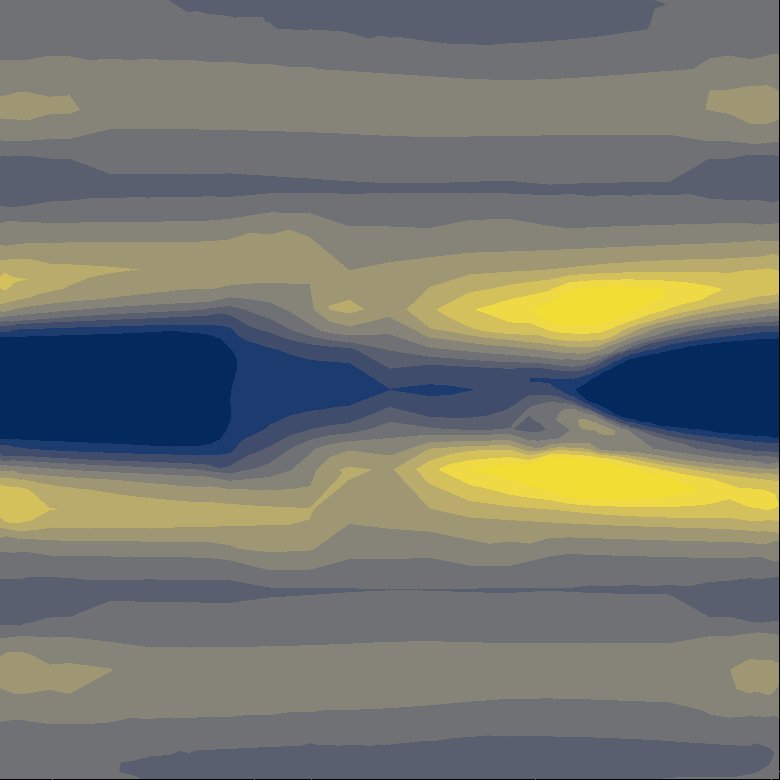
\includegraphics[width=\figfivepanelwidth]{image_2/Figure6/CA_0deg_TKE.png} &
        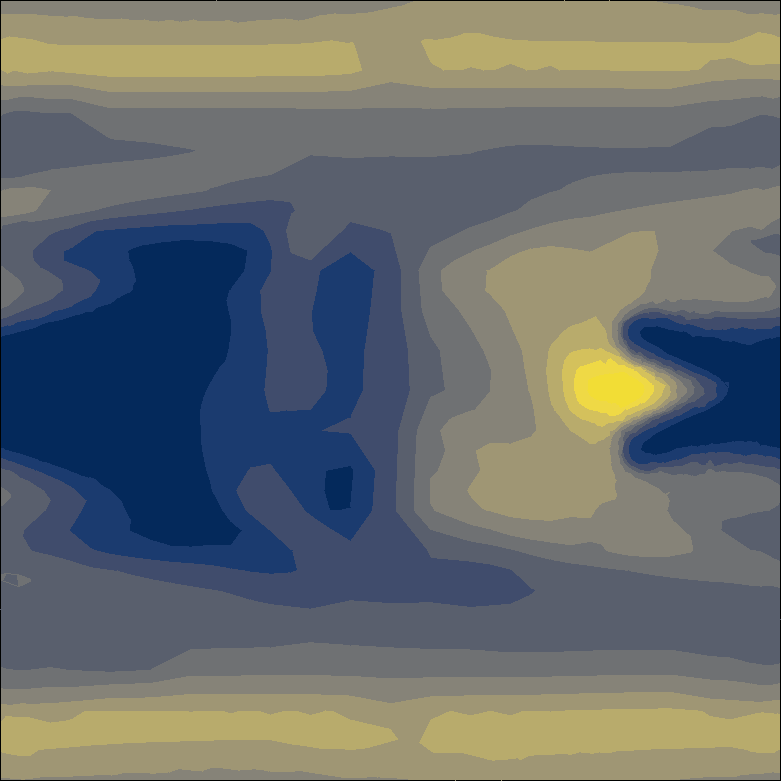
\includegraphics[width=\figfivepanelwidth]{image_2/Figure6/CA_22.5deg_TKE.png} &
        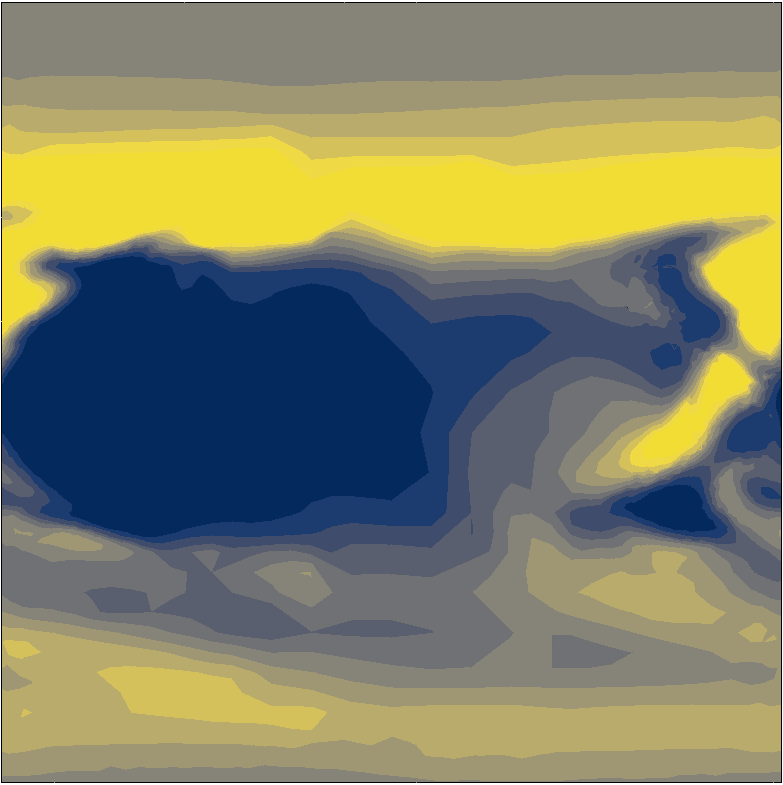
\includegraphics[width=\figfivepanelwidth]{image_2/Figure6/CA_45deg_TKE.png} \\[-1pt]
        {\sffamily\fontsize{7.5}{8.5}\selectfont
         \shortstack[l]{$\times 10^{-3}$\\$\mathrm{m^2\,s^{-2}}$}} &
        \figfivepanellabel{a}{0} &
        \figfivepanellabel{b}{22.5} &
        \figfivepanellabel{c}{45}
    \end{tabular}
    \endgroup
    \caption{TKE distribution of the middle $z$-axis section of CPHE at representative capsule angles ($\theta_c=0\degree$, $22.5\degree$, and $45\degree$).}
    \label{figure5}
\end{figure}


% Figure 6: editable LaTeX layout.
% Change \figuresixpanelwidth or the tabular spacing below to adjust the layout.
\begin{figure}[!ht]
    \centering
    \begingroup
    \newlength{\figuresixpanelwidth}
    \setlength{\figuresixpanelwidth}{0.31\textwidth}

    \tikzset{
        figuresixcallout/.style={
            fill=white,
            fill opacity=0.86,
            text opacity=1,
            rounded corners=0.8pt,
            inner sep=1.2pt,
            align=center,
            font=\sffamily\bfseries\fontsize{5.8}{6.3}\selectfont
        },
        figuresixarrow/.style={
            ->,
            >=stealth,
            draw=black!70,
            line width=0.45pt
        }
    }

    \newcommand{\figuresixlabel}[2]{%
        {\sffamily\bfseries\fontsize{8.5}{9.5}\selectfont
         (#1) $\theta_c=#2^{\circ}$}%
    }

    \newcommand{\figuresixpanel}[3]{%
        \begin{tabular}[t]{@{}c@{}}
            \includegraphics[width=\figuresixpanelwidth]{#1}\\[-1pt]
            \figuresixlabel{#2}{#3}
        \end{tabular}%
    }

    \newcommand{\figuresixpanela}{%
        \begin{tabular}[t]{@{}c@{}}
            \begin{tikzpicture}
                \node[anchor=south west,inner sep=0] (figuresixaimage) at (0,0)
                    {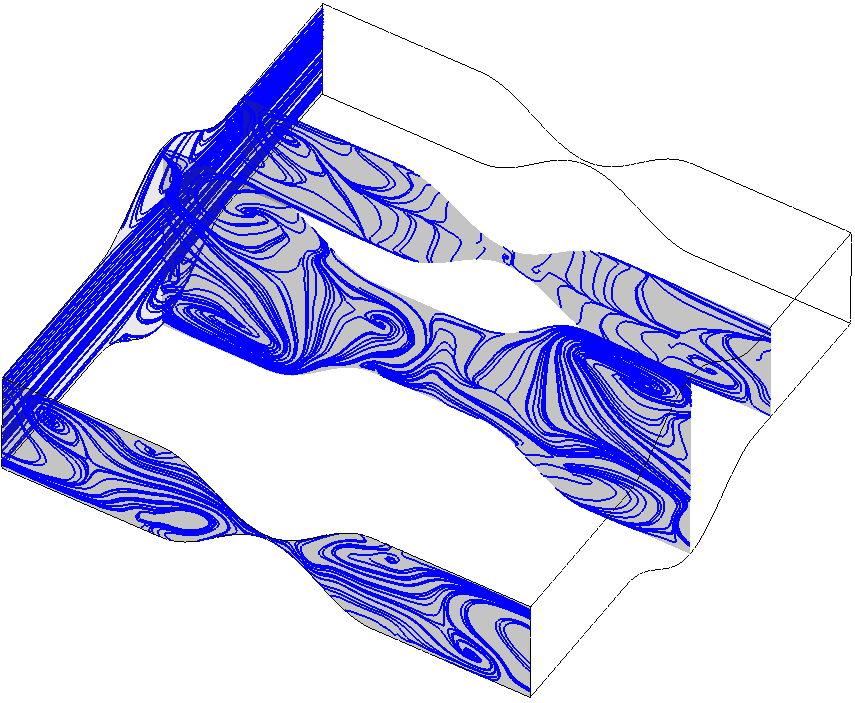
\includegraphics[width=\figuresixpanelwidth]{image_2/Figure7/CA_0deg_2D_stream.png}};
                \begin{scope}[x={(figuresixaimage.south east)},y={(figuresixaimage.north west)}]
                    \node[figuresixcallout] (figuresixwake) at (0.48,0.78)
                        {Wake\\recirculation};
                    \draw[figuresixarrow] (figuresixwake.south west) -- (0.31,0.47);
                \end{scope}
            \end{tikzpicture}\\[-1pt]
            \figuresixlabel{a}{0}
        \end{tabular}%
    }

    \newcommand{\figuresixpanelc}{%
        \begin{tabular}[t]{@{}c@{}}
            \begin{tikzpicture}
                \node[anchor=south west,inner sep=0] (figuresixcimage) at (0,0)
                    {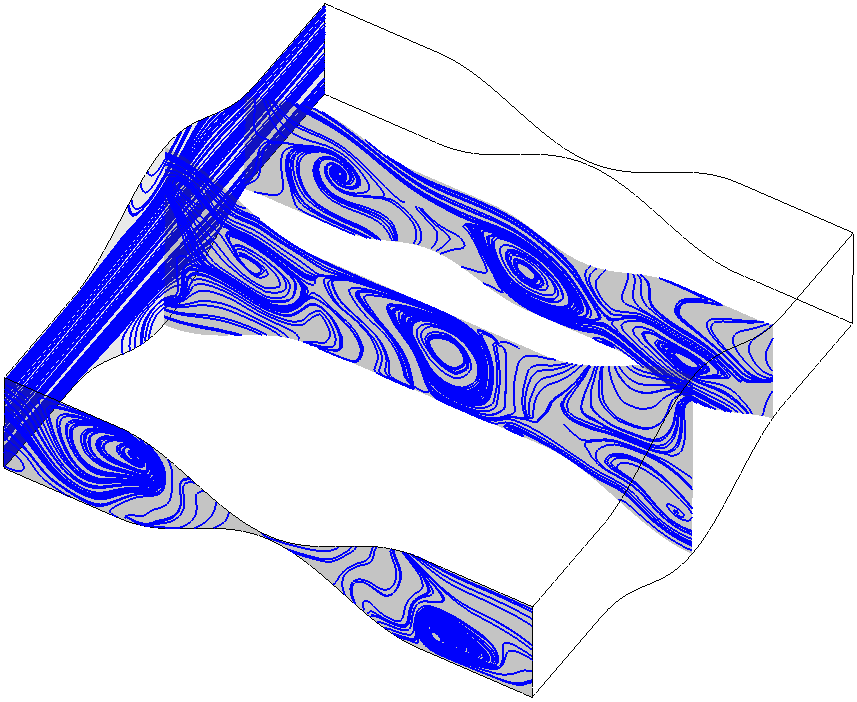
\includegraphics[width=\figuresixpanelwidth]{image_2/Figure7/CA_45deg_2D_stream.png}};
                \begin{scope}[x={(figuresixcimage.south east)},y={(figuresixcimage.north west)}]
                    \node[figuresixcallout] (figuresixreattach) at (0.58,0.79)
                        {Disturbed /\\reattaching flow};
                    \draw[figuresixarrow] (figuresixreattach.south) -- (0.55,0.49);
                \end{scope}
            \end{tikzpicture}\\[-1pt]
            \figuresixlabel{c}{45}
        \end{tabular}%
    }

    \begin{tabular}[c]{@{}c@{\hspace{0.06in}}c@{\hspace{0.06in}}c@{}}
        \figuresixpanela &
        \figuresixpanel{image_2/Figure7/CA_22.5deg_2D_stream.png}{b}{22.5} &
        \figuresixpanelc
    \end{tabular}
    \endgroup
    \caption{2D streamlines of CPHE at representative capsule angles ($\theta_c=0\degree$, $22.5\degree$, and $45\degree$).}
    \label{figure6}
\end{figure}


The response in Figure~\ref{figure4}(a) is nonlinear. Both Nu and $f_F$ reach their largest sampled values at $22.5\degree$ (79.80 and 0.03072), respectively 15.1\% and 87.5\% above the $0\degree$ case. Larger angles do not further increase Nu, despite the more extensive secondary flow. Because $D_e$ varies with angle, the Nu ranking need not match that of the dimensional heat-transfer coefficient or total heat release.

\subsubsection{Capsule height}
\label{sec:disc_capsule_height}

The capsule-height sweep covers $h_c=2$--$5$~mm ($h_c/l_c=0.08$--$0.20$) at $\theta_c=22.5\degree$. Figures~\ref{figure7} and~\ref{figure8} compare TKE and temperature fields at height ratios of 0.08, 0.14, and 0.20.

% Figure 7: editable three-panel LaTeX layout matching Figure 6.
% \figsevenpanelwidth is the final size; no outer scaling is applied.
\begin{figure}[!ht]
    \centering
    \begingroup
    \newlength{\figsevenpanelwidth}
    \newlength{\figsevenlegendunit}
    \setlength{\figsevenpanelwidth}{1.55in}
    \setlength{\figsevenlegendunit}{\dimexpr\figsevenpanelwidth*10/52\relax}

    % Exact RGB values sampled from the updated CFD-Post legend.
    \definecolor{figsevenTKE0}{RGB}{4,41,91}
    \definecolor{figsevenTKE1}{RGB}{27,59,111}
    \definecolor{figsevenTKE2}{RGB}{64,76,108}
    \definecolor{figsevenTKE3}{RGB}{89,95,109}
    \definecolor{figsevenTKE4}{RGB}{111,113,115}
    \definecolor{figsevenTKE5}{RGB}{134,131,120}
    \definecolor{figsevenTKE6}{RGB}{159,150,116}
    \definecolor{figsevenTKE7}{RGB}{184,171,108}
    \definecolor{figsevenTKE8}{RGB}{212,193,92}
    \definecolor{figsevenTKE9}{RGB}{239,217,69}

    \newcommand{\figsevenlegendbar}{%
        \begin{tikzpicture}[baseline=0pt,x=1cm,y=\figsevenlegendunit]
            \fill[figsevenTKE0] (0,0.00) rectangle (0.42,0.52);
            \fill[figsevenTKE1] (0,0.52) rectangle (0.42,1.04);
            \fill[figsevenTKE2] (0,1.04) rectangle (0.42,1.56);
            \fill[figsevenTKE3] (0,1.56) rectangle (0.42,2.08);
            \fill[figsevenTKE4] (0,2.08) rectangle (0.42,2.60);
            \fill[figsevenTKE5] (0,2.60) rectangle (0.42,3.12);
            \fill[figsevenTKE6] (0,3.12) rectangle (0.42,3.64);
            \fill[figsevenTKE7] (0,3.64) rectangle (0.42,4.16);
            \fill[figsevenTKE8] (0,4.16) rectangle (0.42,4.68);
            \fill[figsevenTKE9] (0,4.68) rectangle (0.42,5.20);
            \draw[line width=0.35pt] (0,0) rectangle (0.42,5.20);
            \foreach \y/\ticklabel in {
               0.00/0.0,0.52/1.0,1.04/2.0,1.56/3.0,2.08/4.0,
                2.60/5.0,3.12/6.0,3.64/7.0,4.16/8.0,4.68/9.0,5.20/10.0}
                {\draw[line width=0.3pt] (0.42,\y) -- (0.49,\y)
                 node[anchor=west,font=\sffamily\fontsize{7.5}{8}\selectfont]
                 {\ticklabel};}
        \end{tikzpicture}%
    }

    \newcommand{\figsevenpanellabel}[2]{%
        {\sffamily\bfseries\fontsize{8.5}{9.5}\selectfont
         (#1) $h_c/l_c=#2$}%
    }

    \begin{tabular}[c]{@{}l@{\hspace{0.10in}}c@{\hspace{0.05in}}c@{\hspace{0.05in}}c@{}}
        {\sffamily\bfseries\fontsize{8.5}{9.5}\selectfont
         \shortstack[l]{Turbulence kinetic\\energy, $k$}} & & & \\[-1pt]
        \figsevenlegendbar &
        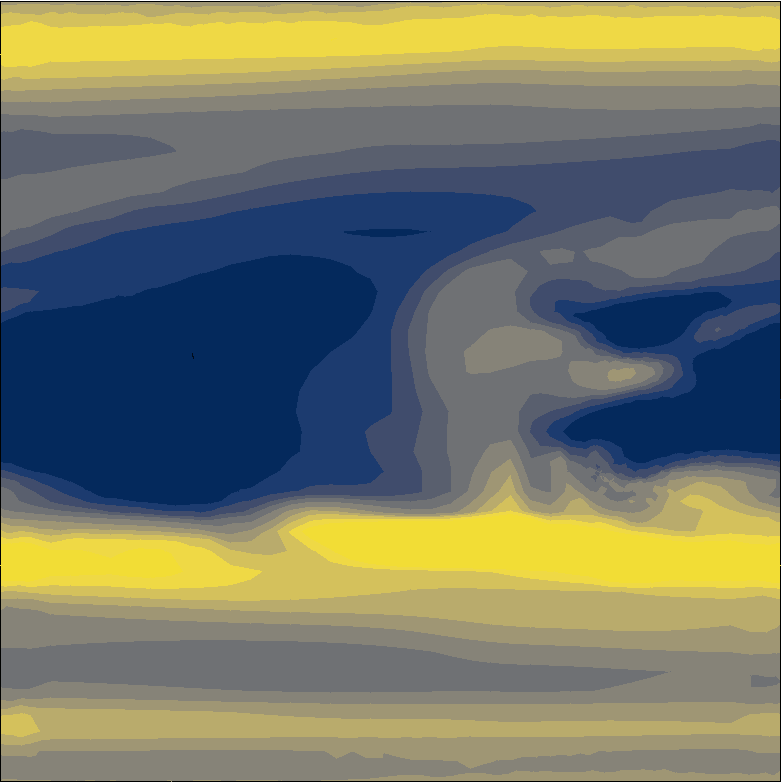
\includegraphics[width=\figsevenpanelwidth]{image_2/Figure9/CH_2mm_TKE.png} &
        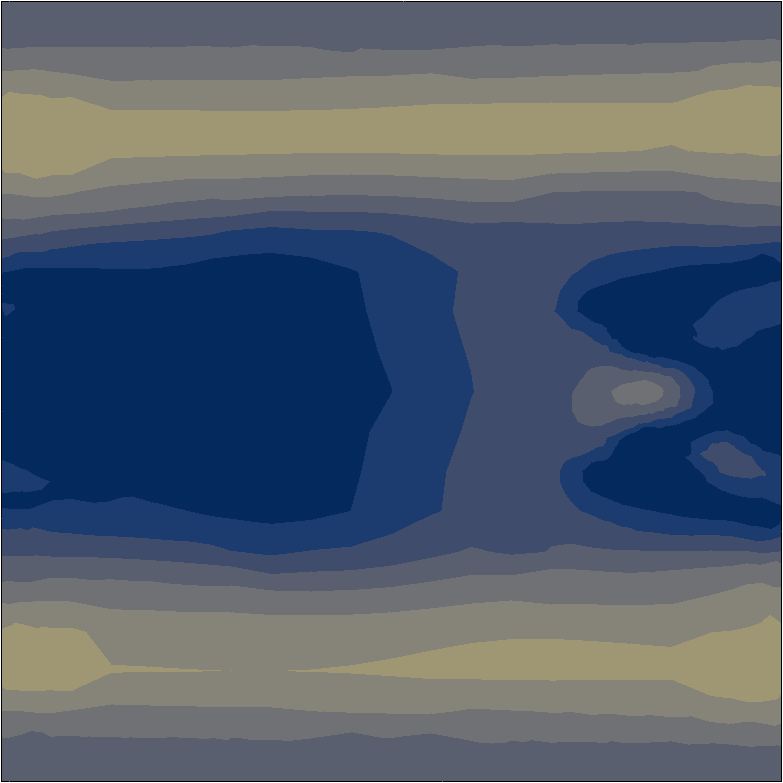
\includegraphics[width=\figsevenpanelwidth]{image_2/Figure9/CH_3.5mm_TKE.png} &
        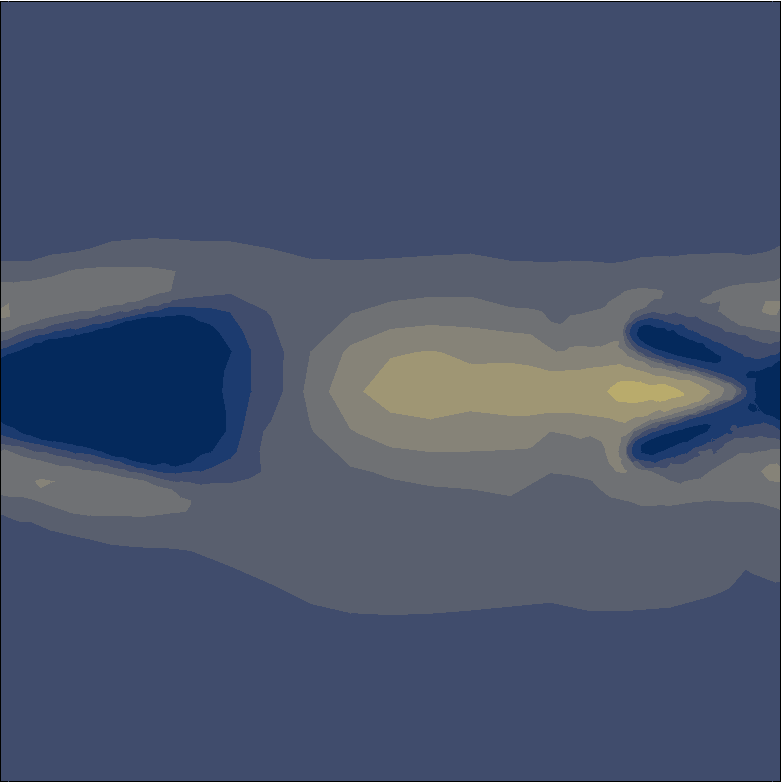
\includegraphics[width=\figsevenpanelwidth]{image_2/Figure9/CH_5mm_TKE.png} \\[-1pt]
        {\sffamily\fontsize{7.5}{8.5}\selectfont
         \shortstack[l]{$\times 10^{-3}$\\$\mathrm{m^2\,s^{-2}}$}} &
        \figsevenpanellabel{a}{0.08} &
        \figsevenpanellabel{b}{0.14} &
        \figsevenpanellabel{c}{0.20}
    \end{tabular}
    \endgroup
    \caption{TKE distribution of the middle $z$-axis section of CPHE at representative normalized capsule heights ($h_c/l_c=0.08$, $0.14$, and $0.20$).}
    \label{figure7}
\end{figure}


As capsule height increases, the broad outer high-TKE lanes in Figure~\ref{figure7} weaken, and the strongest activity becomes concentrated near the central wake. This localization contrasts with a uniform increase in turbulence throughout the channel.

% Figure 8: editable three-panel LaTeX layout matching Figure 4.
% \figeightpanelwidth is the final size; no outer scaling is applied.
\begin{figure}[!ht]
    \centering
    \begingroup
    \newlength{\figeightpanelwidth}
    \newlength{\figeightlegendunit}
    \setlength{\figeightpanelwidth}{1.55in}
    \setlength{\figeightlegendunit}{\dimexpr\figeightpanelwidth*10/52\relax}

    \definecolor{figeightTemp0}{RGB}{70,94,207}
    \definecolor{figeightTemp1}{RGB}{103,136,238}
    \definecolor{figeightTemp2}{RGB}{138,173,253}
    \definecolor{figeightTemp3}{RGB}{173,201,253}
    \definecolor{figeightTemp4}{RGB}{205,217,237}
    \definecolor{figeightTemp5}{RGB}{232,214,205}
    \definecolor{figeightTemp6}{RGB}{246,191,166}
    \definecolor{figeightTemp7}{RGB}{244,157,126}
    \definecolor{figeightTemp8}{RGB}{229,112,88}
    \definecolor{figeightTemp9}{RGB}{201,57,54}

    \newcommand{\figeightlegendbar}{%
        \begin{tikzpicture}[baseline=0pt,x=1cm,y=\figeightlegendunit]
            \fill[figeightTemp0] (0,0.00) rectangle (0.42,0.52);
            \fill[figeightTemp1] (0,0.52) rectangle (0.42,1.04);
            \fill[figeightTemp2] (0,1.04) rectangle (0.42,1.56);
            \fill[figeightTemp3] (0,1.56) rectangle (0.42,2.08);
            \fill[figeightTemp4] (0,2.08) rectangle (0.42,2.60);
            \fill[figeightTemp5] (0,2.60) rectangle (0.42,3.12);
            \fill[figeightTemp6] (0,3.12) rectangle (0.42,3.64);
            \fill[figeightTemp7] (0,3.64) rectangle (0.42,4.16);
            \fill[figeightTemp8] (0,4.16) rectangle (0.42,4.68);
            \fill[figeightTemp9] (0,4.68) rectangle (0.42,5.20);
            \draw[line width=0.35pt] (0,0) rectangle (0.42,5.20);
            \foreach \y/\ticklabel in {
                0.00/293,0.52/294,1.04/295,1.56/296,2.08/297,
                2.60/298,3.12/299,3.64/300,4.16/301,4.68/302,5.20/303}
                {\draw[line width=0.3pt] (0.42,\y) -- (0.49,\y)
                 node[anchor=west,font=\sffamily\fontsize{7.5}{8}\selectfont]
                 {\ticklabel};}
        \end{tikzpicture}%
    }

    \newcommand{\figeightpanellabel}[2]{%
        {\sffamily\bfseries\fontsize{8.5}{9.5}\selectfont
         (#1) $h_c/l_c=#2$}%
    }

    \begin{tabular}[c]{@{}l@{\hspace{0.10in}}c@{\hspace{0.05in}}c@{\hspace{0.05in}}c@{}}
        {\sffamily\bfseries\fontsize{8.5}{9.5}\selectfont Temperature} & & & \\[-1pt]
        \figeightlegendbar &
        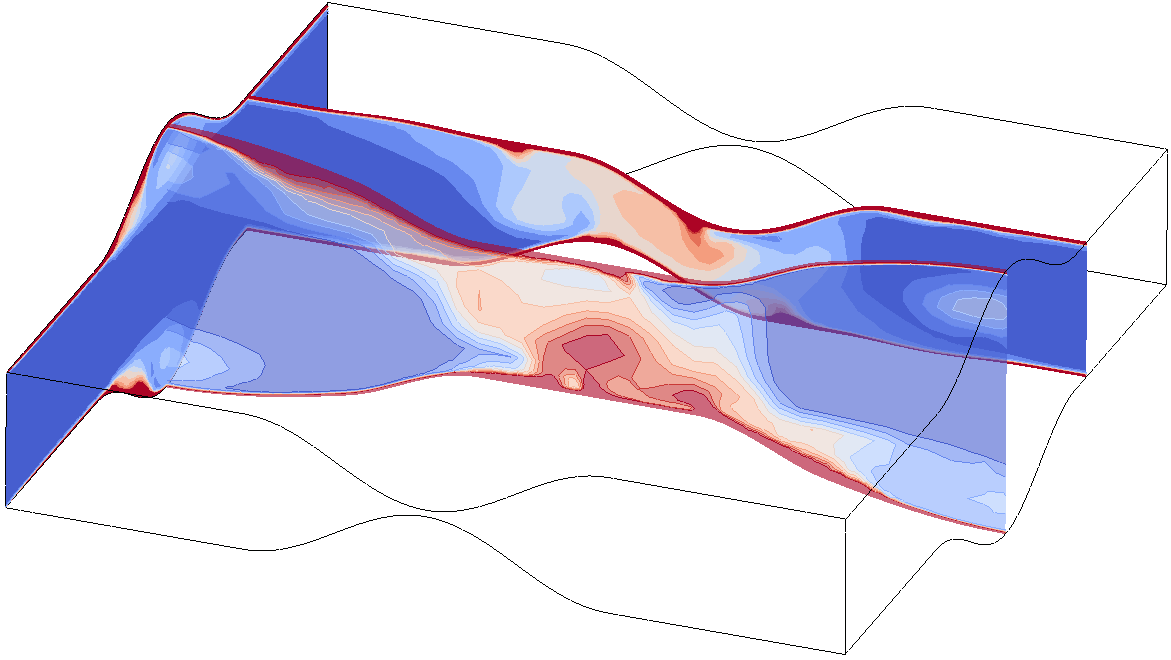
\includegraphics[width=\figeightpanelwidth]{image_2/Figure11/CH_2mm_Temp.png} &
        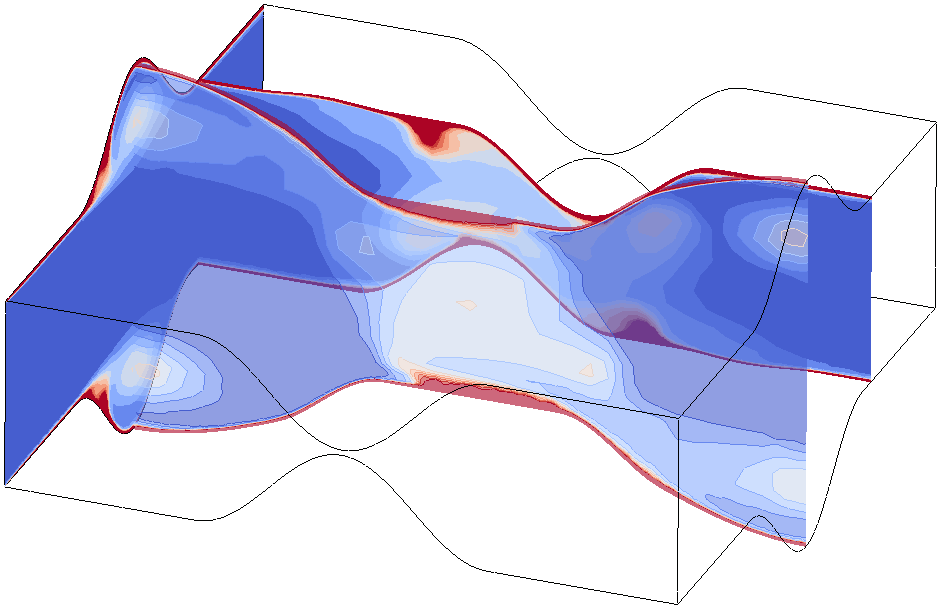
\includegraphics[width=\figeightpanelwidth]{image_2/Figure11/CH_3.5mm_Temp.png} &
        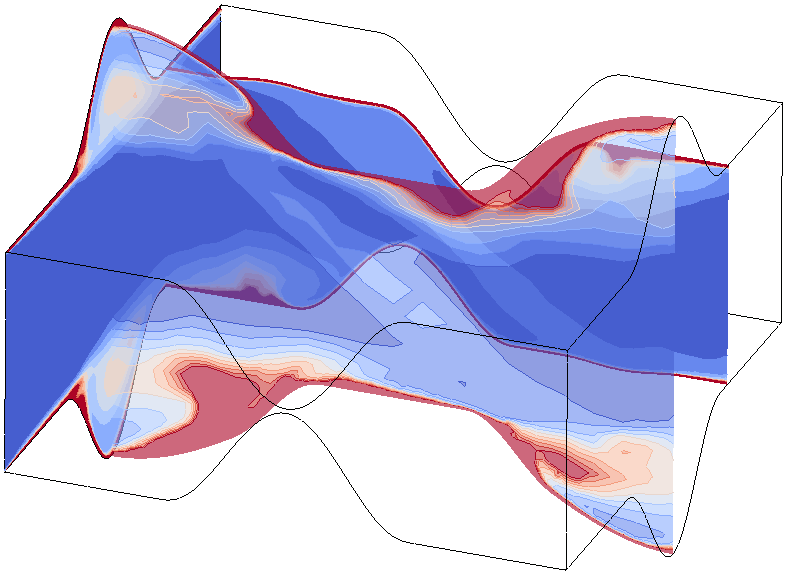
\includegraphics[width=\figeightpanelwidth]{image_2/Figure11/CH_5mm_Temp.png} \\[-1pt]
        {\sffamily\fontsize{7.5}{8.5}\selectfont $[\mathrm{K}]$} &
        \figeightpanellabel{a}{0.08} &
        \figeightpanellabel{b}{0.14} &
        \figeightpanellabel{c}{0.20}
    \end{tabular}
    \endgroup
    \caption{Temperature distribution of CPHE at representative normalized capsule heights ($h_c/l_c=0.08$, $0.14$, and $0.20$).}
    \label{figure8}
\end{figure}


The warmer-fluid regions in Figure~\ref{figure8} shift from the convex-capsule wake towards the concave cavities as height increases, while the channel core remains comparatively cool.

Figure~\ref{figure4}(b) shows an overall but nonlinear increase in Nu with capsule height. The 5~mm capsule gives the highest tested Nu (91.83), whereas the friction factor peaks at 2.5~mm ($f_F=0.03072$). Across the 2--5~mm endpoints, Nu increases by 30.0\% and $f_F$ by 42.3\%.

These normalized trends differ from the dimensional response: as $D_e$ grows and the prescribed speed falls at fixed Re, the mean heat-transfer coefficient, total wall heat rate, and pressure drop all decrease between the endpoints. Higher Nu therefore does not imply greater heat duty in this height sweep.

\subsection{DPHE parametric study}
\label{sec:dphe_results}

The DPHE study varies dimple height and the angle of flow relative to the dimple array.

\subsubsection{Dimple height}
\label{sec:disc_dimple_height}

The dimple-height sweep covers $h_d=2$--$5$~mm ($h_d/l_d=0.08$--$0.20$) at $\theta_d=0\degree$. Figures~\ref{figure9} and~\ref{figure10} compare mid-plane TKE and three-dimensional temperature fields at height ratios of 0.08, 0.14, and 0.20.


% \figninepanelwidth is the final size; no outer scaling is applied.
\begin{figure}[!ht]
    \centering
    \begingroup
    \newlength{\figninepanelwidth}
    \newlength{\figninelegendunit}
    \setlength{\figninepanelwidth}{1.55in}
    \setlength{\figninelegendunit}{\dimexpr\figninepanelwidth*10/52\relax}

    
    \definecolor{fignineTKE0}{RGB}{4,41,91}
    \definecolor{fignineTKE1}{RGB}{27,59,111}
    \definecolor{fignineTKE2}{RGB}{64,76,108}
    \definecolor{fignineTKE3}{RGB}{89,95,109}
    \definecolor{fignineTKE4}{RGB}{111,113,115}
    \definecolor{fignineTKE5}{RGB}{134,131,120}
    \definecolor{fignineTKE6}{RGB}{159,150,116}
    \definecolor{fignineTKE7}{RGB}{184,171,108}
    \definecolor{fignineTKE8}{RGB}{212,193,92}
    \definecolor{fignineTKE9}{RGB}{239,217,69}

    \newcommand{\figninelegendbar}{%
        \begin{tikzpicture}[baseline=0pt,x=1cm,y=\figninelegendunit]
            \fill[fignineTKE0] (0,0.00) rectangle (0.42,0.52);
            \fill[fignineTKE1] (0,0.52) rectangle (0.42,1.04);
            \fill[fignineTKE2] (0,1.04) rectangle (0.42,1.56);
            \fill[fignineTKE3] (0,1.56) rectangle (0.42,2.08);
            \fill[fignineTKE4] (0,2.08) rectangle (0.42,2.60);
            \fill[fignineTKE5] (0,2.60) rectangle (0.42,3.12);
            \fill[fignineTKE6] (0,3.12) rectangle (0.42,3.64);
            \fill[fignineTKE7] (0,3.64) rectangle (0.42,4.16);
            \fill[fignineTKE8] (0,4.16) rectangle (0.42,4.68);
            \fill[fignineTKE9] (0,4.68) rectangle (0.42,5.20);
            \draw[line width=0.35pt] (0,0) rectangle (0.42,5.20);
            \foreach \y/\ticklabel in {
                0.00/0.0,0.52/1.0,1.04/2.0,1.56/3.0,2.08/4.0,
                2.60/5.0,3.12/6.0,3.64/7.0,4.16/8.0,4.68/9.0,5.20/10.0}
                {\draw[line width=0.3pt] (0.42,\y) -- (0.49,\y)
                 node[anchor=west,font=\sffamily\fontsize{7.5}{8}\selectfont]
                 {\ticklabel};}
        \end{tikzpicture}%
    }

    \newcommand{\figninepanellabel}[2]{%
        {\sffamily\bfseries\fontsize{8.5}{9.5}\selectfont
         (#1) $h_d/l_d=#2$}%
    }

    \begin{tabular}[c]{@{}l@{\hspace{0.10in}}c@{\hspace{0.05in}}c@{\hspace{0.05in}}c@{}}
        {\sffamily\bfseries\fontsize{8.5}{9.5}\selectfont
         \shortstack[l]{Turbulence kinetic\\energy, $k$}} & & & \\[-1pt]
        \figninelegendbar &
        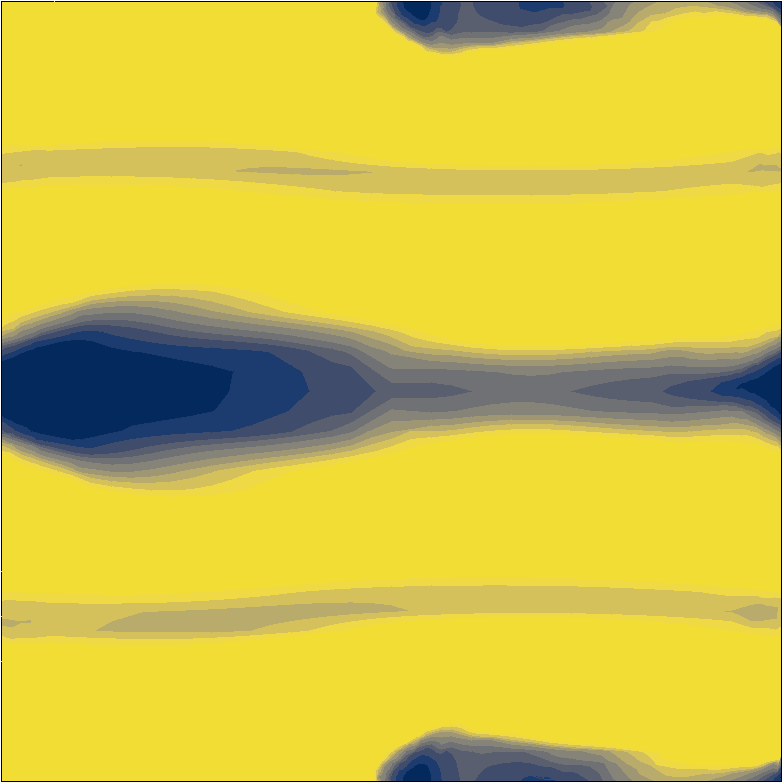
\includegraphics[width=\figninepanelwidth]{image_2/Figure12/DH_2mm_TKE.png} &
        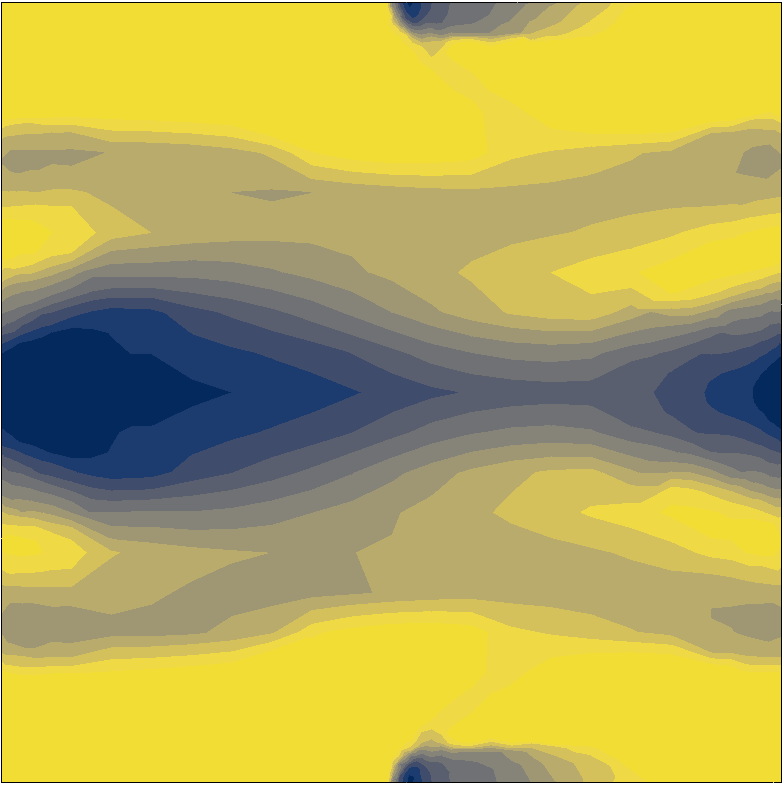
\includegraphics[width=\figninepanelwidth]{image_2/Figure12/DH_3.5mm_TKE.png} &
        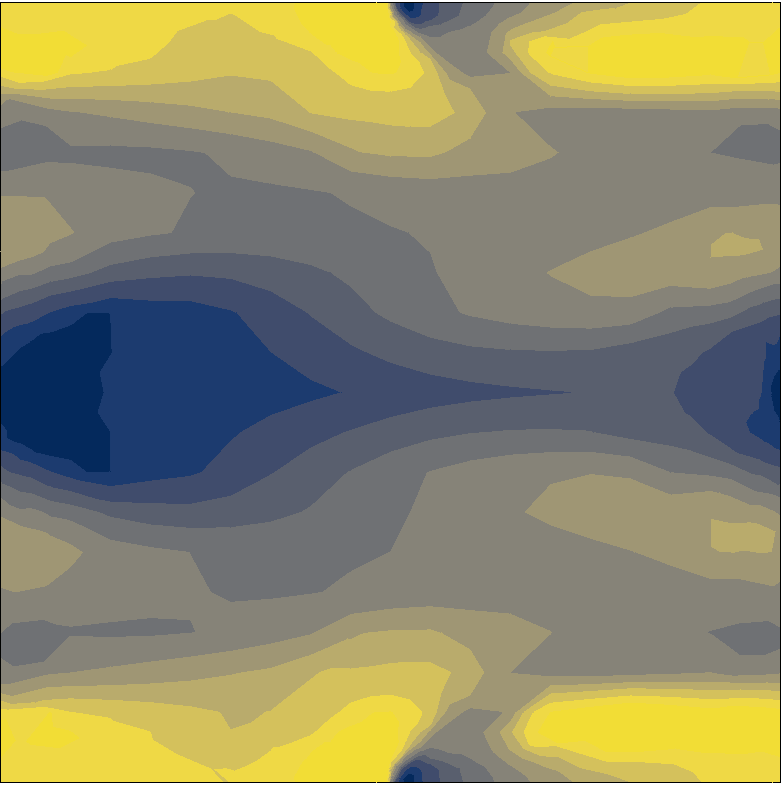
\includegraphics[width=\figninepanelwidth]{image_2/Figure12/DH_5mm_TKE.png} \\[-1pt]
        {\sffamily\fontsize{7.5}{8.5}\selectfont
         \shortstack[l]{$\times 10^{-3}$\\$\mathrm{m^2\,s^{-2}}$}} &
        \figninepanellabel{a}{0.08} &
        \figninepanellabel{b}{0.14} &
        \figninepanellabel{c}{0.20}
    \end{tabular}
    \endgroup
    \caption{TKE distribution of the middle $z$-axis section of DPHE at representative normalized dimple heights ($h_d/l_d=0.08$, $0.14$, and $0.20$).}
    \label{figure9}
\end{figure}


Increasing dimple height localizes the high-TKE regions near the dimple rims and outer boundaries, leaving more of the central passage at low-to-intermediate TKE (Figure~\ref{figure9}). The strongest wake interactions become less spatially extensive rather than producing a section-wide rise in turbulence.

% Figure 10: editable LaTeX layout matching Figure 9.
% \figtenpanelwidth is the final size; no outer scaling is applied.
\begin{figure}[!ht]
    \centering
    \begingroup
    \newlength{\figtenpanelwidth}
    \newlength{\figtenlegendunit}
    \setlength{\figtenpanelwidth}{1.55in}
    \setlength{\figtenlegendunit}{\dimexpr\figtenpanelwidth*10/52\relax}

    % Exact RGB values sampled from the updated CFD-Post legend.
    \definecolor{figtenTemp0}{RGB}{70,94,207}
    \definecolor{figtenTemp1}{RGB}{103,136,238}
    \definecolor{figtenTemp2}{RGB}{138,173,253}
    \definecolor{figtenTemp3}{RGB}{173,201,253}
    \definecolor{figtenTemp4}{RGB}{205,217,237}
    \definecolor{figtenTemp5}{RGB}{232,214,205}
    \definecolor{figtenTemp6}{RGB}{246,191,166}
    \definecolor{figtenTemp7}{RGB}{244,157,126}
    \definecolor{figtenTemp8}{RGB}{229,112,88}
    \definecolor{figtenTemp9}{RGB}{201,57,54}

    \newcommand{\figtenlegendbar}{%
        \begin{tikzpicture}[baseline=0pt,x=1cm,y=\figtenlegendunit]
            \fill[figtenTemp0] (0,0.00) rectangle (0.42,0.52);
            \fill[figtenTemp1] (0,0.52) rectangle (0.42,1.04);
            \fill[figtenTemp2] (0,1.04) rectangle (0.42,1.56);
            \fill[figtenTemp3] (0,1.56) rectangle (0.42,2.08);
            \fill[figtenTemp4] (0,2.08) rectangle (0.42,2.60);
            \fill[figtenTemp5] (0,2.60) rectangle (0.42,3.12);
            \fill[figtenTemp6] (0,3.12) rectangle (0.42,3.64);
            \fill[figtenTemp7] (0,3.64) rectangle (0.42,4.16);
            \fill[figtenTemp8] (0,4.16) rectangle (0.42,4.68);
            \fill[figtenTemp9] (0,4.68) rectangle (0.42,5.20);
            \draw[line width=0.35pt] (0,0) rectangle (0.42,5.20);
            \foreach \y/\ticklabel in {
                0.00/293,0.52/294,1.04/295,1.56/296,2.08/297,
                2.60/298,3.12/299,3.64/300,4.16/301,4.68/302,5.20/303}
                {\draw[line width=0.3pt] (0.42,\y) -- (0.49,\y)
                 node[anchor=west,font=\sffamily\fontsize{7.5}{8}\selectfont]
                 {\ticklabel};}
        \end{tikzpicture}%
    }

    \newcommand{\figtenpanellabel}[2]{%
        {\sffamily\bfseries\fontsize{8.5}{9.5}\selectfont
         (#1) $h_d/l_d=#2$}%
    }

    \begin{tabular}[c]{@{}l@{\hspace{0.10in}}c@{\hspace{0.05in}}c@{\hspace{0.05in}}c@{}}
        {\sffamily\bfseries\fontsize{8.5}{9.5}\selectfont Temperature} & & & \\[-1pt]
        \figtenlegendbar &
        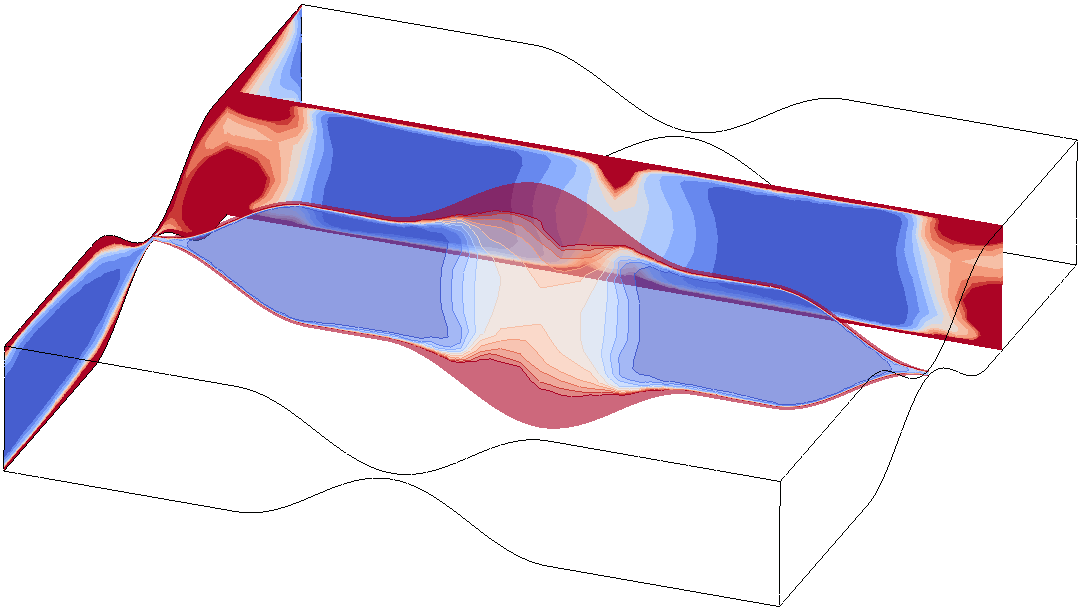
\includegraphics[width=\figtenpanelwidth]{image_2/Figure14/DH_2mm_Temp.png} &
        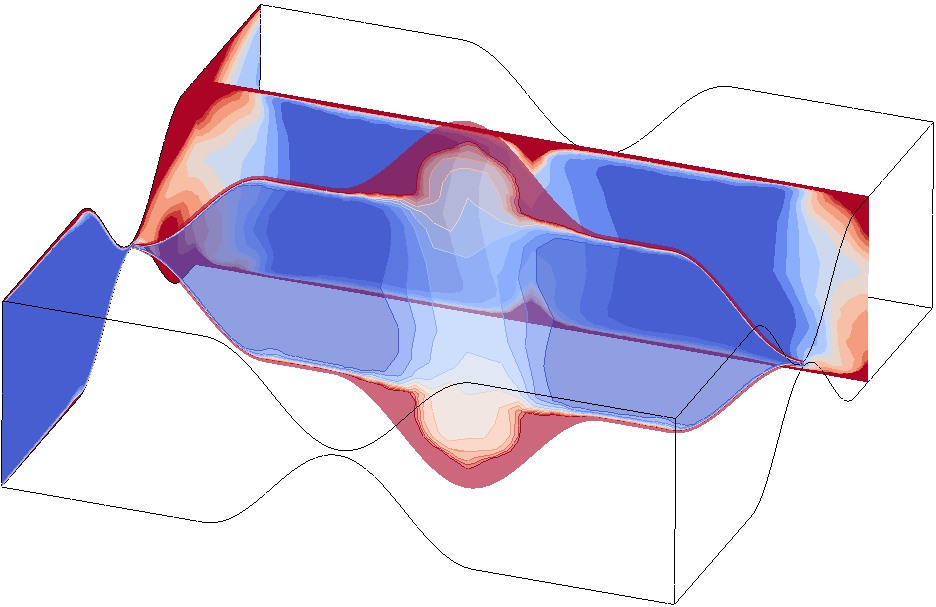
\includegraphics[width=\figtenpanelwidth]{image_2/Figure14/DH_3.5mm_Temp.png} &
        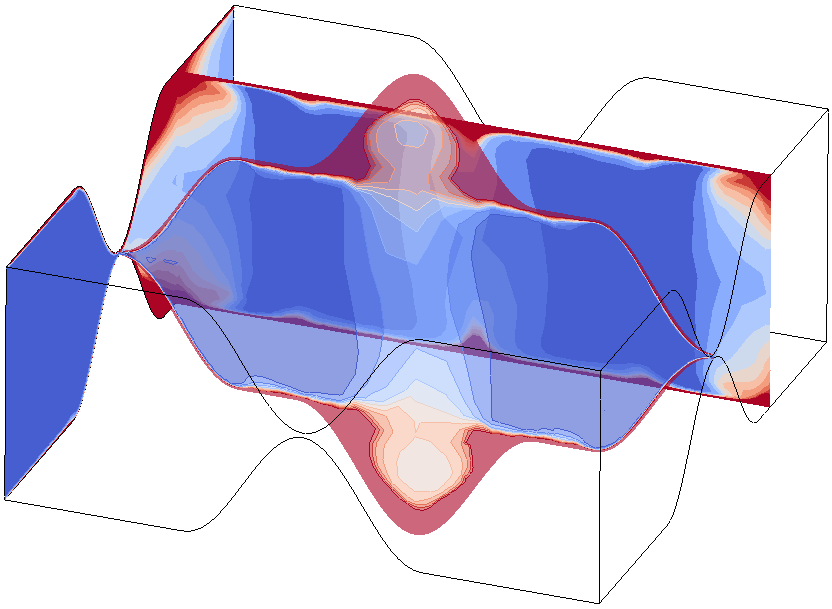
\includegraphics[width=\figtenpanelwidth]{image_2/Figure14/DH_5mm_Temp.png} \\[-1pt]
        {\sffamily\fontsize{7.5}{8.5}\selectfont $[\mathrm{K}]$} &
        \figtenpanellabel{a}{0.08} &
        \figtenpanellabel{b}{0.14} &
        \figtenpanellabel{c}{0.20}
    \end{tabular}
    \endgroup
    \caption{3D temperature distribution of DPHE at representative normalized dimple heights ($h_d/l_d=0.08$, $0.14$, and $0.20$).}
    \label{figure10}
\end{figure}


In Figure~\ref{figure10}, the warmed-fluid plume extends farther across the passage as dimple height increases. This shows how heating is redistributed between the opposing surfaces, not an increase in the wall-integrated heat rate.

Unlike the capsule-height sweep, both Nu and $f_F$ increase monotonically with dimple height (Figure~\ref{figure4}(b)). Across 2--5~mm, Nu increases by 62.7\% to 104.09, while $f_F$ increases by 169.7\% to 0.07133. The relative rise in friction is therefore substantially larger than that in Nu. As in the capsule-height sweep, however, increasing $D_e$ and decreasing speed at fixed Re accompany lower dimensional heat-transfer coefficients, total wall heat rates, and pressure drops between the endpoints.

\subsubsection{Dimple angle}
\label{sec:disc_dimple_angle}

Although each circular dimple is axisymmetric, changing the flow direction relative to the array alters the interaction between neighbouring convex and concave wakes \citep{jiang2019a, hamedi2024}. Figure~\ref{figure11} compares TKE at $\theta_d=0\degree$, $22.5\degree$, and $45\degree$. The nearly symmetric low-TKE corridor at $0\degree$ becomes an oblique wake bordered by a concentrated high-TKE band at $22.5\degree$. At $45\degree$, a coherent diagonal corridor forms, with high TKE more localized near the dimples.



\begin{figure}[!ht]
    \centering
    \begingroup
    \newlength{\figelevenpanelwidth}
    \newlength{\figelevenlegendunit}
    \setlength{\figelevenpanelwidth}{1.55in}
    \setlength{\figelevenlegendunit}{\dimexpr\figelevenpanelwidth*10/52\relax}

  
    \definecolor{figelevenTKE0}{RGB}{4,41,91}
    \definecolor{figelevenTKE1}{RGB}{27,59,111}
    \definecolor{figelevenTKE2}{RGB}{64,76,108}
    \definecolor{figelevenTKE3}{RGB}{89,95,109}
    \definecolor{figelevenTKE4}{RGB}{111,113,115}
    \definecolor{figelevenTKE5}{RGB}{134,131,120}
    \definecolor{figelevenTKE6}{RGB}{159,150,116}
    \definecolor{figelevenTKE7}{RGB}{184,171,108}
    \definecolor{figelevenTKE8}{RGB}{212,193,92}
    \definecolor{figelevenTKE9}{RGB}{239,217,69}

    \newcommand{\figelevenlegendbar}{%
        \begin{tikzpicture}[baseline=0pt,x=1cm,y=\figelevenlegendunit]
            \fill[figelevenTKE0] (0,0.00) rectangle (0.42,0.52);
            \fill[figelevenTKE1] (0,0.52) rectangle (0.42,1.04);
            \fill[figelevenTKE2] (0,1.04) rectangle (0.42,1.56);
            \fill[figelevenTKE3] (0,1.56) rectangle (0.42,2.08);
            \fill[figelevenTKE4] (0,2.08) rectangle (0.42,2.60);
            \fill[figelevenTKE5] (0,2.60) rectangle (0.42,3.12);
            \fill[figelevenTKE6] (0,3.12) rectangle (0.42,3.64);
            \fill[figelevenTKE7] (0,3.64) rectangle (0.42,4.16);
            \fill[figelevenTKE8] (0,4.16) rectangle (0.42,4.68);
            \fill[figelevenTKE9] (0,4.68) rectangle (0.42,5.20);
            \draw[line width=0.35pt] (0,0) rectangle (0.42,5.20);
            \foreach \y/\ticklabel in {
                0.00/0.0,0.52/1.0,1.04/2.0,1.56/3.0,2.08/4.0,
                2.60/5.0,3.12/6.0,3.64/7.0,4.16/8.0,4.68/9.0,5.20/10.0}
                {\draw[line width=0.3pt] (0.42,\y) -- (0.49,\y)
                 node[anchor=west,font=\sffamily\fontsize{7.5}{8}\selectfont]
                 {\ticklabel};}
        \end{tikzpicture}%
    }

    \newcommand{\figelevenpanellabel}[2]{%
        {\sffamily\bfseries\fontsize{8.5}{9.5}\selectfont
         (#1) $\theta_d=#2\degree$}%
    }

    \begin{tabular}[c]{@{}l@{\hspace{0.10in}}c@{\hspace{0.05in}}c@{\hspace{0.05in}}c@{}}
        {\sffamily\bfseries\fontsize{8.5}{9.5}\selectfont
         \shortstack[l]{Turbulence kinetic\\energy, $k$}} & & & \\[-1pt]
        \figelevenlegendbar &
        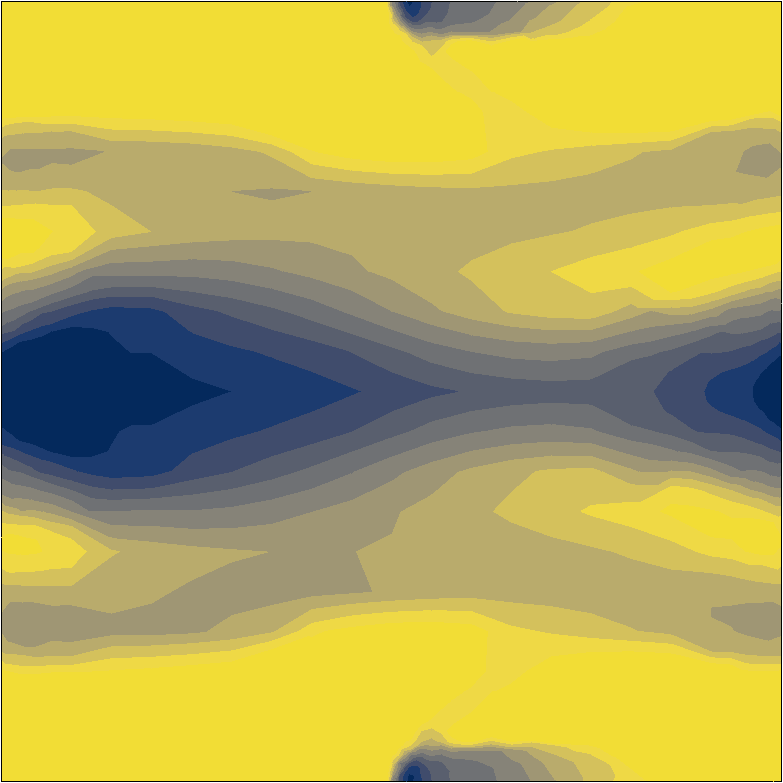
\includegraphics[width=\figelevenpanelwidth]{image_2/Figure15/DA_0deg_TKE.png} &
        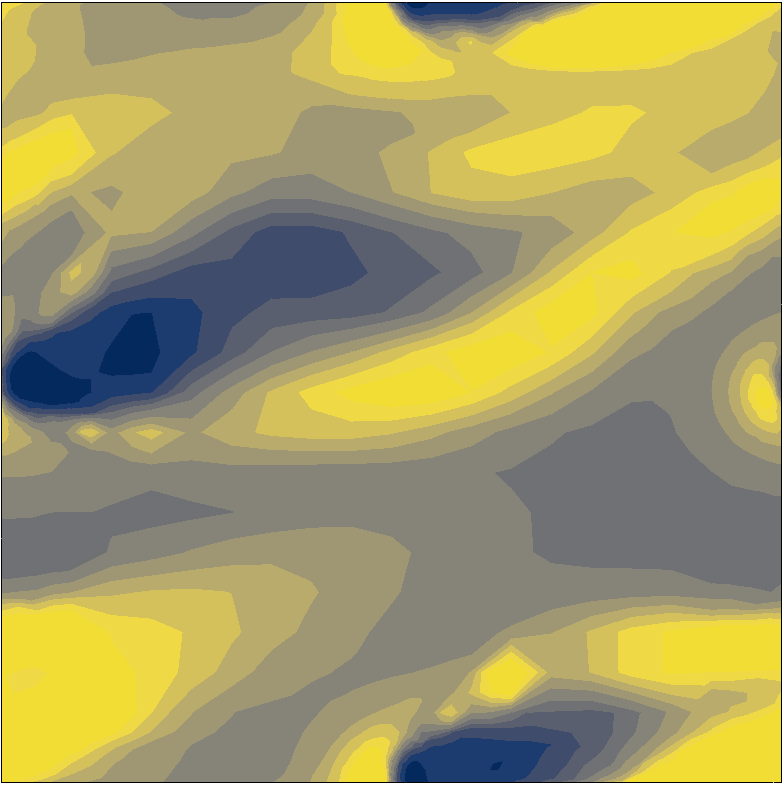
\includegraphics[width=\figelevenpanelwidth]{image_2/Figure15/DA_22.5deg_TKE.png} &
        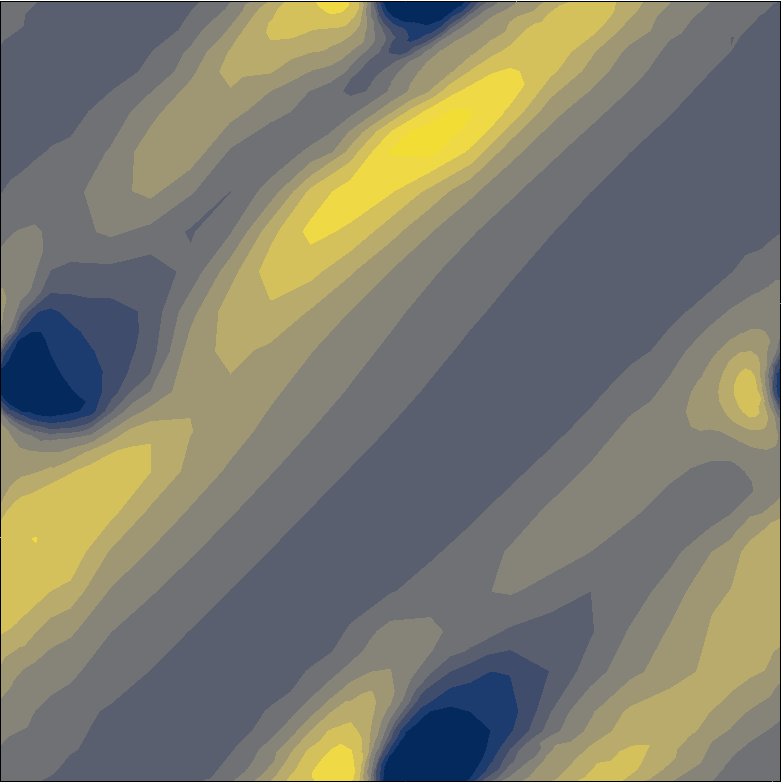
\includegraphics[width=\figelevenpanelwidth]{image_2/Figure15/DA_45deg_TKE.png} \\[-1pt]
        {\sffamily\fontsize{7.5}{8.5}\selectfont
         \shortstack[l]{$\times 10^{-3}$\\$\mathrm{m^2\,s^{-2}}$}} &
        \figelevenpanellabel{a}{0} &
        \figelevenpanellabel{b}{22.5} &
        \figelevenpanellabel{c}{45}
    \end{tabular}
    \endgroup
    \caption{TKE distribution of the middle $z$-axis section of DPHE at representative angles of flow ($\theta_d=0\degree$, $22.5\degree$, and $45\degree$).}
    \label{figure11}
\end{figure}


\begin{figure}[!ht]
    \centering
    \begingroup
    \newlength{\figtwelvepanelwidth}
    \setlength{\figtwelvepanelwidth}{0.31\textwidth}

    \newcommand{\figtwelvelabel}[2]{%
        {\sffamily\bfseries\fontsize{8.5}{9.5}\selectfont
         (#1) $\theta_d=#2\degree$}%
    }

    \newcommand{\figtwelvepanel}[3]{%
        \begin{tabular}[t]{@{}c@{}}
            \includegraphics[width=\figtwelvepanelwidth]{#1}\\[-1pt]
            \figtwelvelabel{#2}{#3}
        \end{tabular}%
    }

    \begin{tabular}[c]{@{}c@{\hspace{0.05in}}c@{\hspace{0.05in}}c@{}}
        \figtwelvepanel{image_2/Figure16/DA_0deg_2D_stream.png}{a}{0} &
        \figtwelvepanel{image_2/Figure16/DA_22.5deg_2D_stream.png}{b}{22.5} &
        \figtwelvepanel{image_2/Figure16/DA_45deg_2D_stream.png}{c}{45}
    \end{tabular}
    \endgroup
    \caption{2D streamlines of DPHE at representative angles of flow ($\theta_d=0\degree$, $22.5\degree$, and $45\degree$).}
    \label{figure12}
\end{figure}


The streamlines in Figure~\ref{figure12} show compact, locally confined recirculation at $0\degree$, larger structures interacting with the oblique through-flow at $22.5\degree$, and a more coherent diagonal passage at $45\degree$. The latter bypasses much of the stronger wake interaction, consistent with reduced resistance and heat transfer.

Figure~\ref{figure4}(a) shows a non-monotonic response: Nu peaks at $30\degree$ (106.37), while $f_F$ peaks at $22.5\degree$ (0.06503). The 2.6\% Nu difference between these angles does not establish a resolved optimum without quantified numerical uncertainty. Both measures decline beyond $30\degree$, reaching their lowest values at $45\degree$: Nu is 9.6\% and $f_F$ is 59.2\% below the $0\degree$ values. Because $D_e$ and the reference speed remain fixed in this sweep, these trends also track the mean heat-transfer coefficient and pressure drop.

\subsection{Cross-parameter thermo-geometric comparison}
\label{sec:tgg_comparison}

Figures~\ref{figure13} and~\ref{figure14} compare the constructed PEC values for the angle and normalized-height sweeps. All three PEC plots, including Figure~\ref{figure15}, use the same two-wall coefficient and case-specific fluid-domain mass-average reference convention, together with the prescribed-Reynolds-number velocity defined in Section~\ref{sec:numerical_methods}. The 29 case labels contain 27 distinct saved solutions because two sweep reference points are shared. The dimple-angle sweep reaches its highest PEC at $\theta_d=45\degree$ (285.19). The targeted combined case therefore pairs this angle with $h_d=5.0$~mm instead of the angle sweep's fixed height of 3.5~mm.

\noindent% Figure 13: focused PEC comparison for the angle sweeps.
\begin{minipage}[t]{0.485\linewidth}
    \centering
    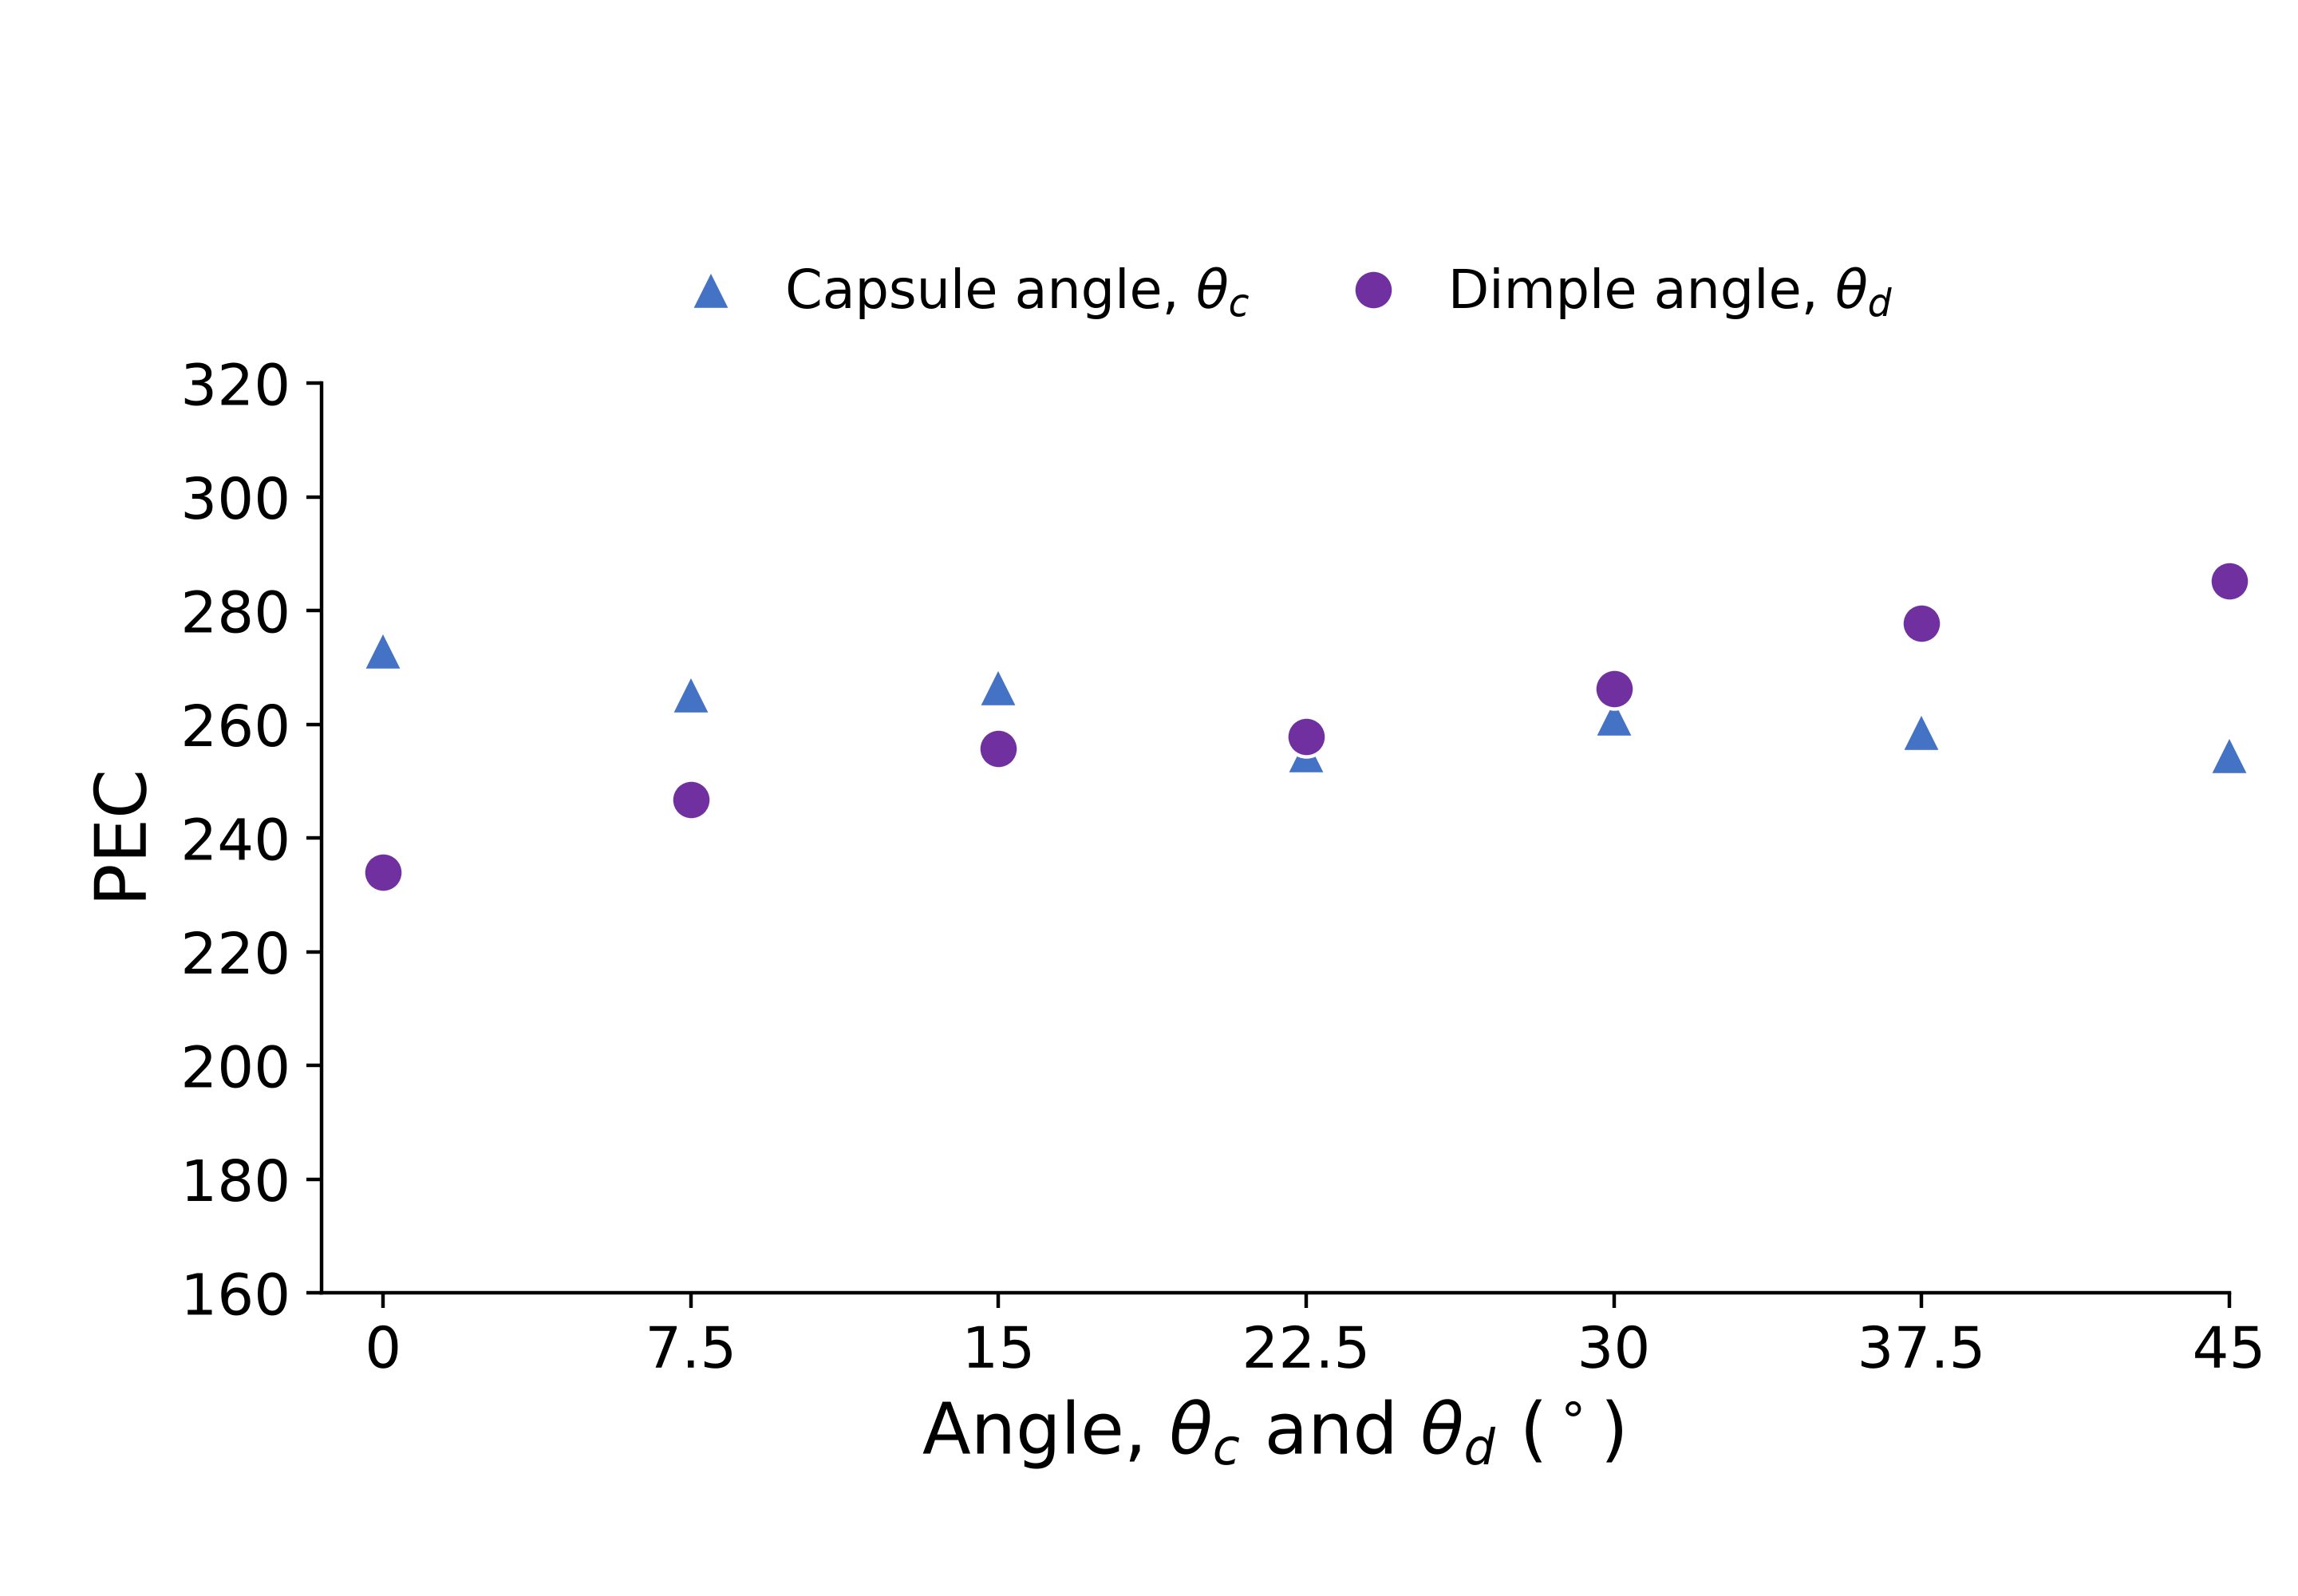
\includegraphics[
        width=\linewidth,
        keepaspectratio,
        interpolate=true
    ]{media/Figure13_PEC_angle.png}
    \captionsetup{hypcap=false}
    \captionof{figure}{Two-wall PEC referenced to the fluid-domain mass-average temperature for the angle sweeps: $h_c=2.5$~mm and $h_d=3.5$~mm.}
    \label{figure13}
\end{minipage}%
\hfill% Figure 14: focused PEC comparison for the normalized-height sweeps.
\begin{minipage}[t]{0.485\linewidth}
    \centering
    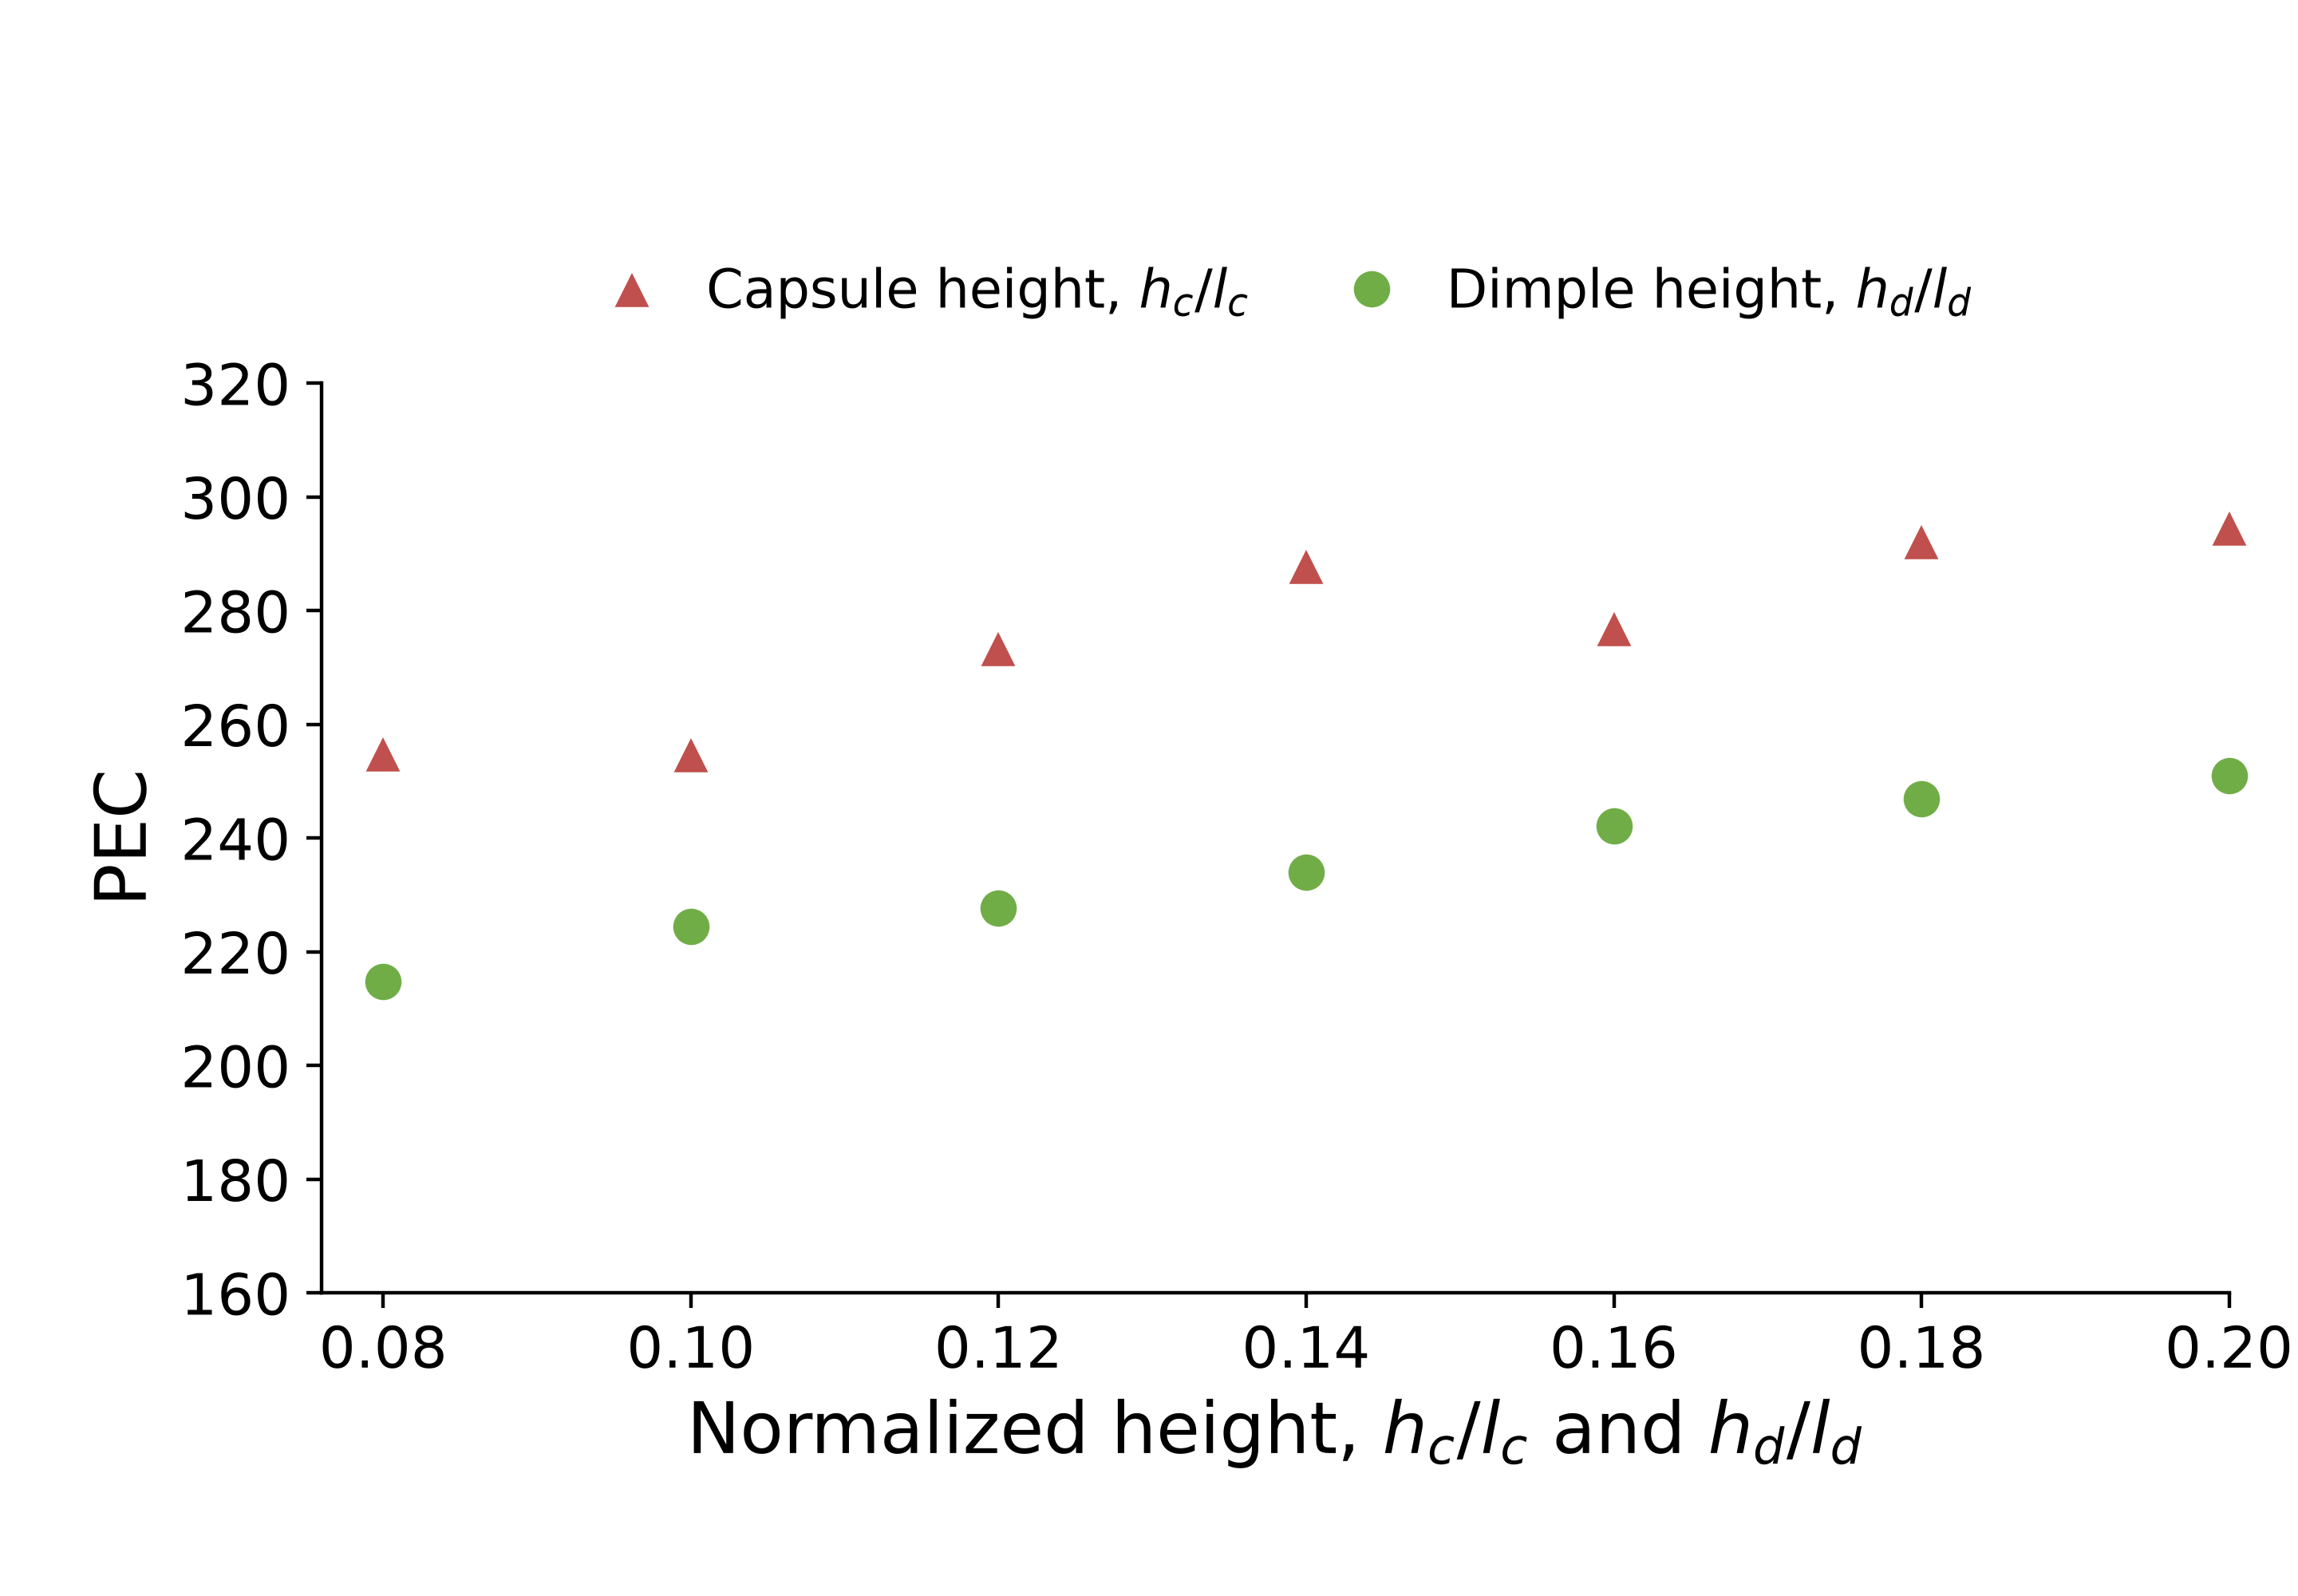
\includegraphics[
        width=\linewidth,
        keepaspectratio,
        interpolate=true
    ]{media/Figure14_PEC_height.png}
    \captionsetup{hypcap=false}
    \captionof{figure}{Two-wall PEC referenced to the fluid-domain mass-average temperature for the height sweeps: $\theta_c=22.5\degree$ and $\theta_d=0\degree$.}
    \label{figure14}
\end{minipage}%

\par\vspace{\baselineskip}

To quantify the paired separation in Figures~\ref{figure13} and~\ref{figure14}, the matched-case PEC difference is defined as
\begin{equation}
  \Delta\mathrm{PEC}=\mathrm{PEC}_{\mathrm{CPHE}}-\mathrm{PEC}_{\mathrm{DPHE}},
  \label{eq:delta-pec}
\end{equation}
where positive values indicate a higher CPHE score on the stated reporting basis. Equation~\eqref{eq:delta-pec} is a paired-difference definition introduced here. Ordinary least-squares regression \citep{nistLinearRegression} of the seven matched numerical angles gives
\begin{equation}
  \Delta\mathrm{PEC}_{\theta}=33.695-1.42984\left(\frac{\theta}{1\degree}\right),
  \qquad 0\degree\leq\theta\leq45\degree,
  \label{eq:delta-pec-angle}
\end{equation}
with $R^2=0.973$ and $\mathrm{RMSE}=\sqrt{\sum_{i=1}^{7}e_i^2/7}=3.54$, where $e_i$ is the fitted residual. The actual endpoint differences are 39.04 at $0\degree$ and $-30.61$ at $45\degree$; the paired differences decrease across the seven sampled angles. The fitted coefficients are results of the present reconstruction; the cited source supplies the regression method, not these coefficients.

For the seven matched normalized heights, $h_c/l_c=h_d/l_d=0.08$--$0.20$, $\Delta\mathrm{PEC}_h$ remains positive but scattered. Its mean is 42.01, sample standard deviation 7.77 and range 30.36--53.94. A linear height fit has only $R^2=0.087$, so the height result is reported as a descriptive offset. The angle fit is an empirical summary of seven paired cases, not an independently validated predictive correlation; neither its $R^2$ nor its RMSE quantifies CFD uncertainty.

These results are limited to the present one-factor sweeps at $\mathrm{Re}=4282$: the angle comparison pairs the CPHE cases at $h_c=2.5$~mm with the DPHE cases at $h_d=3.5$~mm, and the height comparison pairs the CPHE cases at $\theta_c=22.5\degree$ with the DPHE cases at $\theta_d=0\degree$. They do not describe angle--height interactions and should not be extrapolated to other Reynolds numbers, unit-cell geometries, fluids, or boundary conditions.

\begin{figure}[!ht]
  \centering
  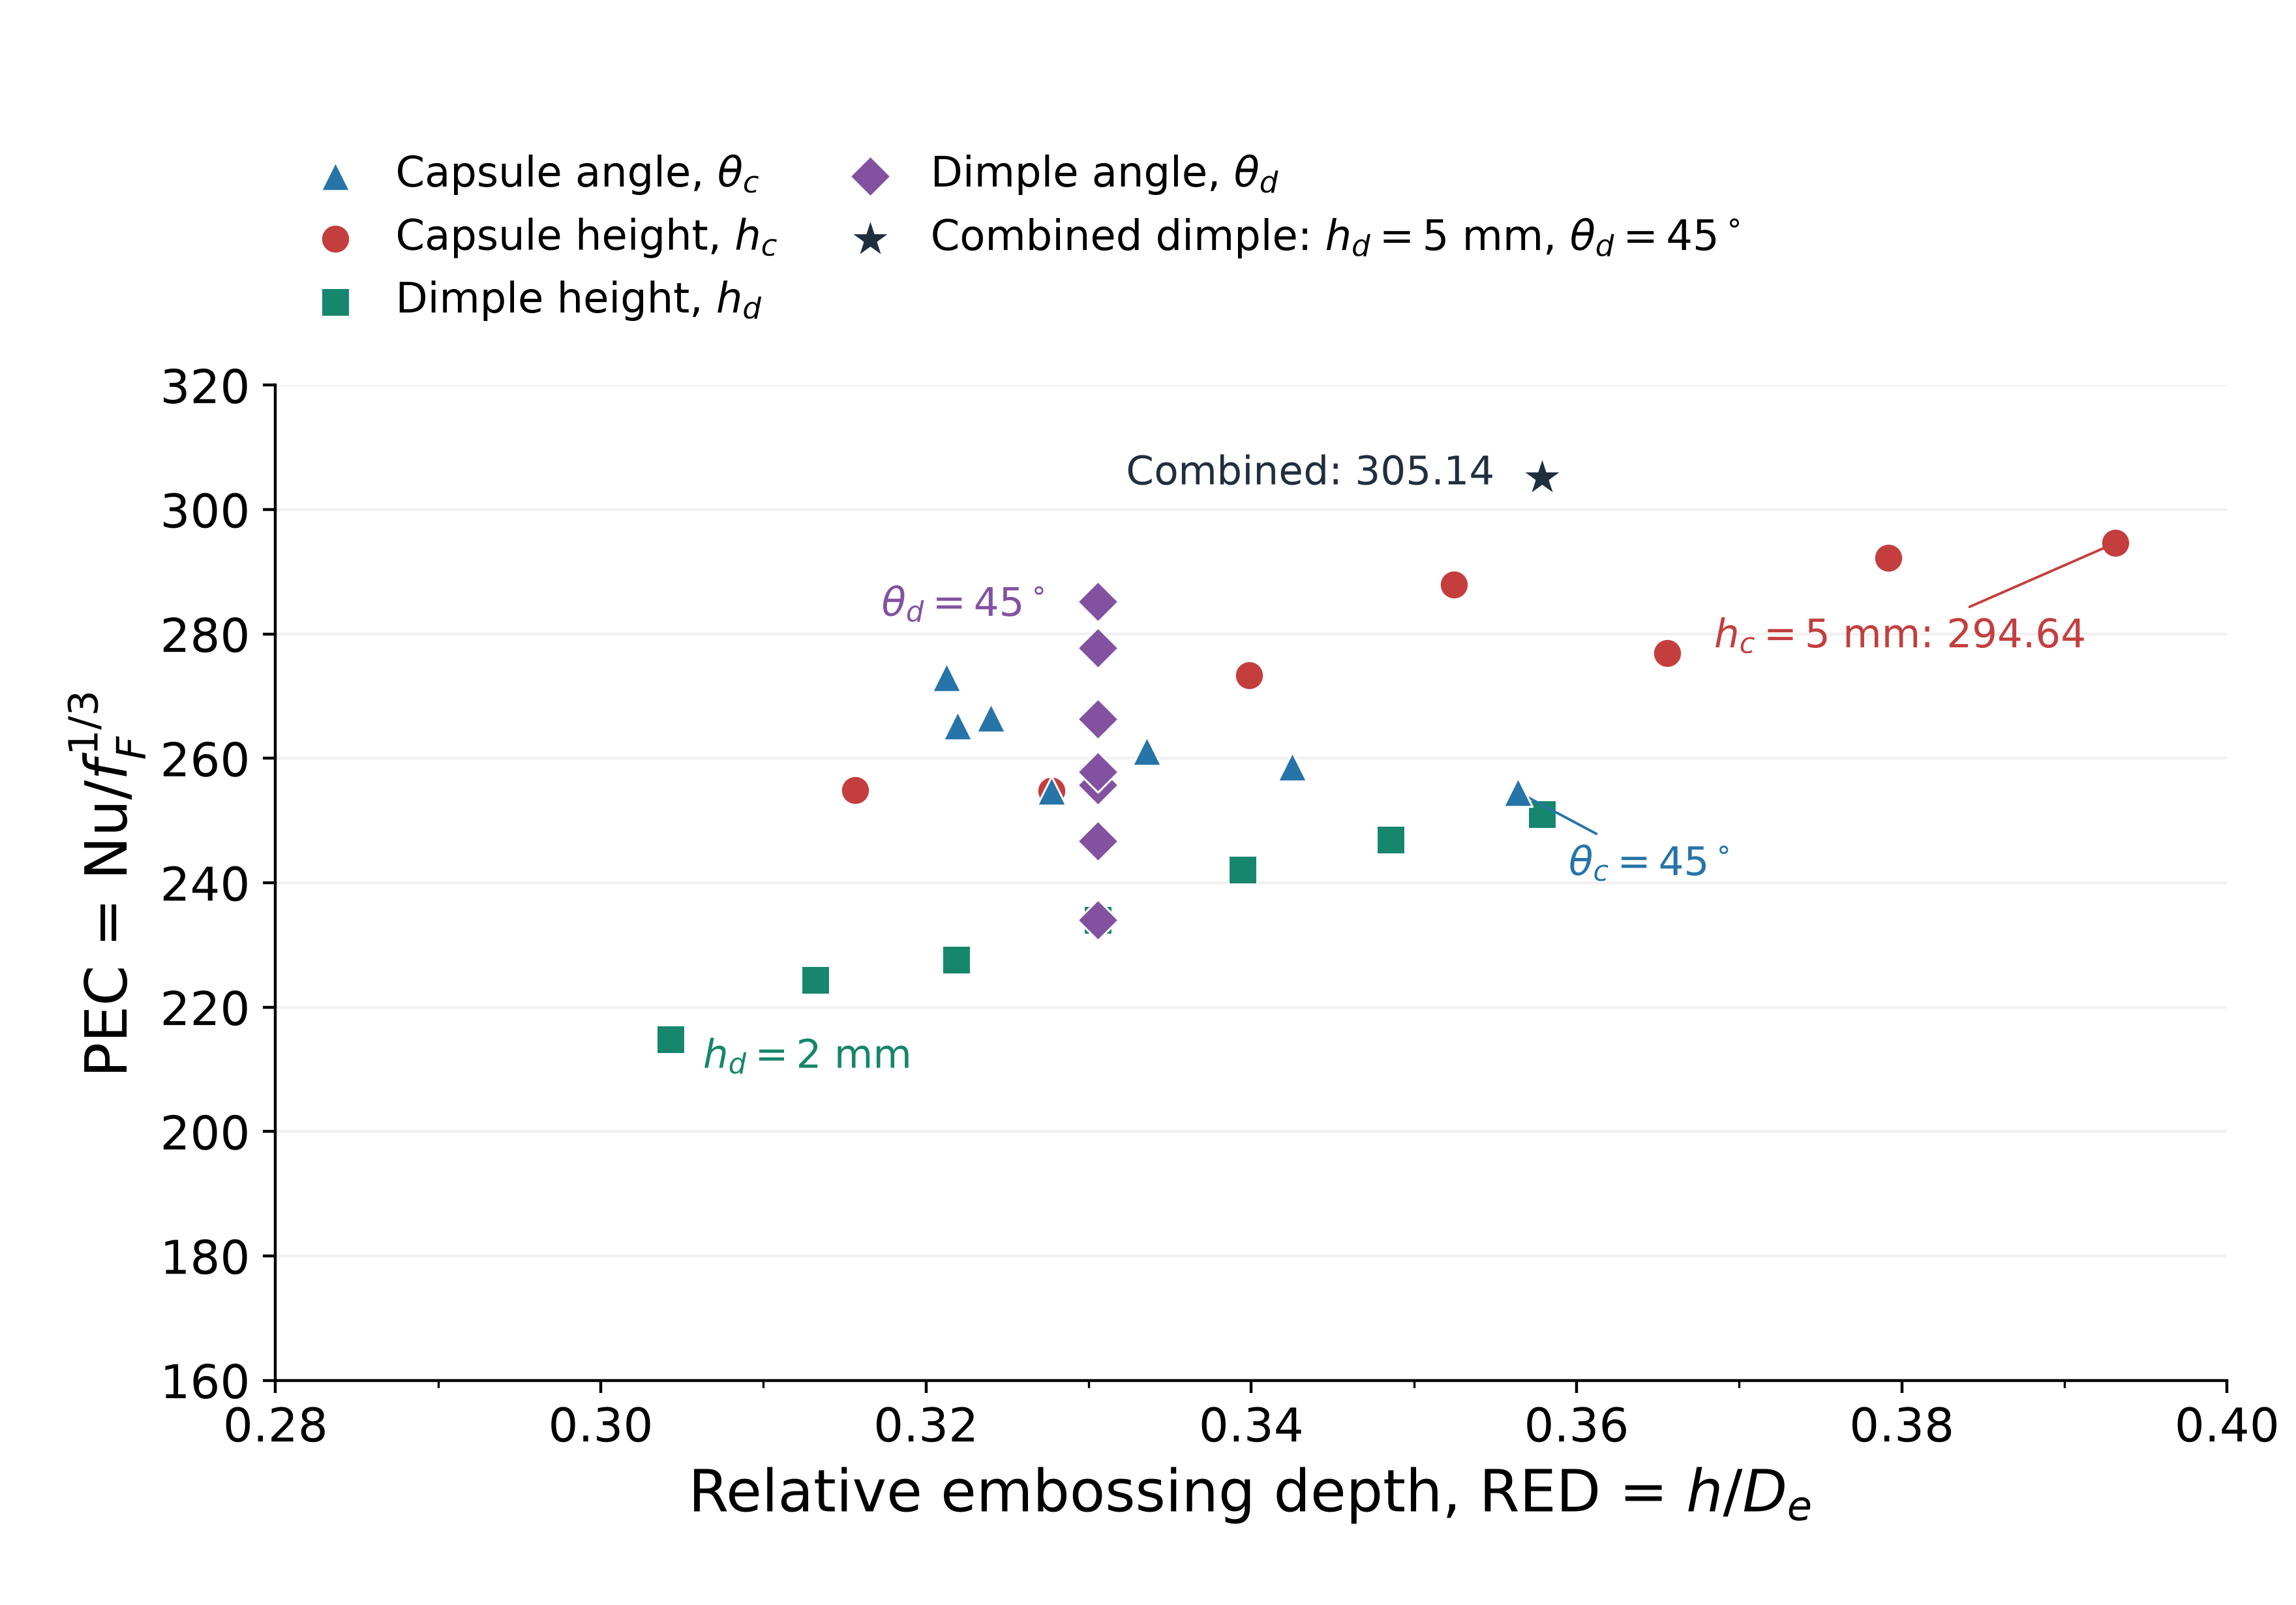
\includegraphics[
    width=0.9\linewidth,
    keepaspectratio,
    interpolate=true
  ]{media/PEC_Vs_RED.png}
  \caption{Performance evaluation criterion (PEC\,=\,Nu/$f_F^{1/3}$) versus relative embossing depth (\texorpdfstring{RED\,=\,$h/D_e$}{RED = h/De}). The star denotes $\theta_d=45\degree$, $h_d=5.0$~mm. All scores use both heated walls and case-specific $T_{\mathrm{ref}}=T_{f,ave}$, the fluid-domain mass-average temperature. These are constructed unit-cell scores, not thermally fully developed coefficients or uncertainty-resolved rankings.}
  \label{figure15}
\end{figure}


Figures~\ref{figure13}--\ref{figure15} use a single saved-field postprocessing basis: $D_e=4A_0L/(S_1+S_2)$, $U=4282\mu/(\rho D_e)$, and $h_{ave}=(Q_1+Q_2)/[(S_1+S_2)(T_w-T_{f,ave})]$ with $T_{\mathrm{ref}}=T_{f,ave}$ evaluated as the mass-weighted volume average of static temperature over the entire fluid domain of each case. Thus both walls enter the heat-transfer coefficient as well as the hydraulic-diameter definition. The prescribed reference velocity is corroborated by the finite embedded inlet profiles, including the combined case; its non-finite saved inlet velocity-component arrays are not used in this reconstruction. No wall heat rate, flow field or physical boundary condition has been changed.

The constructed two-wall PEC ranges are 254.6--273.0 for capsule angle, 254.8--294.6 for capsule height, 214.8--251.0 for dimple height, and 234.0--285.2 for dimple angle. The combined dimple case gives RED\,=\,0.357856, Nu\,=\,87.38, $f_F=0.023480$, and PEC\,=\,305.14. It has the highest constructed score, followed by the $h_c=5.0$~mm capsule case at PEC\,=\,294.64. Their separation is 3.56\%; without quantified numerical uncertainty, this is not interpreted as a resolved superiority or a global optimum. Height sweeps span different RED values, and the measured capsule-angle hydraulic diameter also changes. All dimple-angle cases share the same geometry and RED, so RED alone cannot identify the flow-entry angle. These scores characterize the saved, thermally developing unit-cell heating problem with periodic hydrodynamics; they do not establish thermally fully developed periodic heat transfer.

\subsection{Limitations of this study}
\label{sec:limitations}

Exploring the intricacies of heat exchanger designs through numerical investigations can be incredibly enlightening, yet it is important to remember these methods are not without their flaws. Recognizing these limitations helps us better understand the results and spot areas that need more research and real-world testing.

For instance, our study assumes that the working fluid does not compress, making the calculations simpler. However, this assumption does not hold up for all real-world scenarios, especially when dealing with gases or other compressible fluids. Additionally, our simulations only consider single-phase flow, meaning they do not take into account the complexities that come with multiphase flows like liquid-gas, or solid-liquid. These interactions can drastically change heat transfer and pressure drops. Moreover, the boundary conditions we apply in simulations tend to be idealized. They do not always reflect the varied and sometimes chaotic conditions found in real-life operations, such as changing inlet temperatures or pressures, and leakage or local geometry variations. We also assume that the physical properties of the working fluid, like density, viscosity, and thermal conductivity, remain constant. In reality, these properties can change significantly with temperature and pressure, which affects both flow and heat transfer.

Section~\ref{sec:du-validation} reports two quasi-periodic Nusselt numbers with a provisional comparison table targeting the D3 projected-area (PA) data of Du et al. The mean absolute reported difference is $2.03\%$ across all four points are arithmetic against the supplied digitisation, whose coordinates were not fully reproduced by an independent reading of the original plot. Reference-data reconciliation, four further study points, the numerical-verification record, and consistency of area, temperature, property and diameter definitions remain incomplete. The table therefore does not establish experimental validation of the full parametric study or an uncertainty-qualified accuracy bound.


\section{Conclusions}
\label{sec:conclusion}

The central contribution of this study is a direct, side-by-side comparison of capsule-type (CPHE) and dimple-type (DPHE) channels under a common numerical and operating baseline. It addresses the comparison gap left by separate studies with differing conditions and reporting definitions. Both surface families were assessed using the same steady-state, single-phase water-flow RANS framework, unit-cell approach, thermal boundary conditions and performance definitions at $\mathrm{Re}=4282$. Four seven-case, one-factor sweeps examined capsule angle ($\theta_c$), capsule height ($h_c$), dimple height ($h_d$), and dimple flow-entry angle ($\theta_d$), with one targeted combined dimple case. The comparative contribution lies in quantifying the geometry-dependent thermal--hydraulic trade-offs across both surface families using established Nu, Fanning friction and PEC measures, supported by the computed flow and temperature fields.

Across the 2--5~mm height endpoints, capsule Nu and $f_F$ increase by 30.0\% and 42.3\%, respectively, compared with 62.7\% and 169.7\% for dimples. These paired changes quantify the different normalized heat-transfer--resistance responses of the two height sweeps. They are not increases in absolute heat duty or pressure drop, because the hydraulic diameter and reference speed also vary at fixed Re.

On the common two-wall, case-specific fluid-domain mass-average reference basis, capsule-angle PEC spans 254.6--273.0, while capsule-height PEC spans 254.8--294.6. The dimple-angle and dimple-height ranges are 234.0--285.2 and 214.8--251.0, respectively. The highest capsule-height score occurs at $h_c=5.0$~mm. These differences apply to the prescribed reference-speed, hydraulic-diameter and coefficient definitions used in this comparison.

For matched numerical angles, the least-squares descriptor is $\Delta\mathrm{PEC}_{\theta}=33.695-1.42984(\theta/1\degree)$ with $R^2=0.973$ and RMSE 3.54 over $0\degree$--$45\degree$. The actual paired differences decrease across the sampled angles. Matched normalized-height differences remain positive, averaging 42.01 with a sample standard deviation of 7.77 across $h/l=0.08$--$0.20$; their linear fit has $R^2=0.087$. These are descriptive results for the tested one-factor cases, not validated correlations for other geometries or operating conditions.

The targeted combination $\theta_d=45\degree$, $h_d=5.0$~mm gives PEC = 305.14, the highest constructed score. It is 6.99\% above the corresponding 3.5~mm dimple-angle case and 21.57\% above the 5.0~mm dimple-height case at $0\degree$. Its score is 3.56\% above the 5.0~mm capsule case (294.64); a numerically resolved superiority is not established without quantified uncertainty.

These findings are specific to the tested $0\degree$--$45\degree$ angles, 2--5~mm heights, water properties, $\mathrm{Re}=4282$ and unit-cell boundary conditions. Four one-factor sweeps and one combined case do not establish a global optimum across untested parameter interactions. The thermal results characterize heating with a prescribed inlet temperature and a streamwise quasi-periodic iteration loop for velocity and turbulence profiles; they do not establish thermal periodicity. Completion of the D3--PA validation benchmark on a consistent reporting basis, together with quantified uncertainties and tests at further Reynolds numbers, heights, angles and fluids, remains necessary.

\authorcontributions{Both C.S.C. and C.S. have similar contributions to the paper and are acknowledged as the first authors. Conceptualization, S.V. and L.S.; methodology, S.V., K.I., A.D. and J.T.; software, C.S.C. and C.S.; formal analysis, C.S.C. and C.S.; investigation, C.S.C. and C.S.; resources, L.S.; data curation, C.S.C. and C.S.; writing: original draft preparation, C.S.C. and C.S.; writing: review and editing, S.V., A.D. and K.I.; visualization, C.S.C. and C.S.; supervision, L.S., S.V., K.I., J.T, and A.D.; project administration, S.V.. All authors have read and agreed to the submitted version of the manuscript.}

\funding{This research received no external funding}

\institutionalreview{Not applicable}

\informedconsent{Not applicable}

\dataavailability{The data presented in this study are available on request from the corresponding author}

\acknowledgments{InKorr Pty Ltd. provided resources for this research}

\conflictsofinterest{Author Mr. Lance Smith was employed by the company InKorr Pty Ltd, Melbourne, Australia.
The remaining authors declare that the research was conducted in the absence of any commercial or financial relationships that could be construed as a potential conflict of interest.}

\useofartificialintelligence{AI or AI-assisted tools were not used in drafting any aspect of this manuscript}


% Keep references aligned with the local review margins.
\reftitle{References}
\bibliography{references,energies_revision_sources}
\PublishersNote{}
\end{document}
